\documentclass{DeustoFDP}

\usepackage{hologo} % Paquete no necesario. Borrar en la memoria final al sustituir el texto
\usepackage{eurosym}
\usepackage[toc, acronym, nomain]{glossaries}

\setlength{\headheight}{12.22504pt}

\hypersetup{
  pdfauthor={Jesus María Sesma Solance},
  pdftitle={Gesti\'on de repositorios sem\'anticos compatibles con el est\'andar OAI-PMH},
}

\bibliography{bibliografia}
\makeglossaries

\begin{document}

\newacronym{xml}{XML}{Extensible Markup Language}
\newacronym[longplural={Bases de Datos}]{bd}{BD}{Base de Datos}
\newacronym{dbms}{DBMS}{Database Management Systems}
\newacronym{http}{HTTP}{Hypertext Transfer Protocol}
\newacronym{rmbp}{rMBP}{Retina Macbook Pro}
\newacronym{oai}{OAI}{Open Archives Initiative}
\newacronym{oaipmh}{OAI-PMH}{Open Archives Initiative Protocol for Metadata Harvesting}
\newacronym{dms}{DMS}{Data Management System}
\newacronym{api}{API}{Application Programming Interface}
\newacronym{html}{HTML}{HyperText Markup Language}
\newacronym{css}{CSS}{Cascading Style Sheets}
\newacronym{js}{JS}{JavaScript}
\newacronym{sql}{SQL}{Structured Query Language}
\newacronym{sparql}{SPARQL}{SPARQL Protocol and RDF Query Language}
\newacronym{dc}{DC}{Dublin Core}
\newacronym{labman}{LabMan}{Laboratory Management}
\newacronym{cms}{CMS}{Content Management System}
\newacronym{lod}{LOD}{Linked Open Data}
\newacronym{ld}{LD}{Linked Data}
\newacronym{csv}{CSV}{Comma Separated Values}
\newacronym{uri}{URI}{Uniform Resource Identifier}
\newacronym{url}{URL}{Uniform Resource Locator}
\newacronym{rdf}{RDF}{Resource Description Framework}
\newacronym{ansi}{ANSI}{American National Standards Institute}
\newacronym{iso}{ISO}{Internaltiona Organization for Standardization}
\newacronym{w3c}{W3C}{World Wide Web Consortium}
\newacronym{dawg}{DAWG}{Data Access Working Group}
\newacronym{ldap}{LDAP}{Lightweight Directory Access Protocol}
\newacronym{xpath}{XPath}{XML Path}
\newacronym{xquery}{XQuery}{XML Query}
\newacronym{s2s}{S2S}{SPARQL-to-SQL}

\frontmatter 
\pagestyle{plain}

% Las siguientes lineas (21--26) se pueden eliminar del documento final.
% Notese que en ese caso es necesario descomentar la linea 28 para que las
% paginas esten correctamente numeradas.
\begin{titlepage} 
  \newgeometry{left=0cm,right=0cm,bottom=0cm,top=0cm}
  
\includegraphics{fig/portada_rendered}
  \restoregeometry
\end{titlepage}
\cleardoublepage

%\setcounter{page}{3}

\chapter*{Resumen}

Deustotech cree que es posible contribuir a un mundo mejor mediante el uso de
las tecnologías de Internet y las Telecomunicaciones.

Como resultado de este pensamiento nació \acrshort{labman}, un sistema de gestión de grupo de investigación. Esta aplicación web tiene como objetivo gestionar toda la información referente a los investigadores, proyectos, publicaciones y tesis de un grupo relacionada entre si. Permite 
generar diversas gráficas que permiten analizar de forma rápida la evolución y desempeño del equipo
de investigación.
Este aplicativo en un claro ejemplo de una web de datos de nueva generación de portales web, dónde
no solo se exportan documentos, sino que habilita la exportación de datos y \acrshortpl{api}, que
tienen como propósito facilitar la explotación de recursos.

Aunque el sistema es capaz de exportar esta información semántica, todavía se ve la necesidad de que este colabore con sistemas imperantes en la industria para el intercambio de información de recursos académicos y científicos.
Es por ello que se requiere dar soporte a \acrshort{oai}, mediante la implementación de su protocolo \acrshort{oaipmh}, con el fin de dar servicio a las soluciones del sector que apostaron en su día por esta tecnología. Así mismo, se desea desarrollar un estudio sobre ventajas e inconvenientes que supone cada una de las tecnologías que usa LabMan para la explotación de la información, siendo estas \acrshort{sql} y \acrshort{sparql} en la actualidad y \acrshort{oaipmh} tras el despliegue en producción de este proyecto. Para finalizar este estudio, se dispondrá una conclusión general y la justificación de la tecnología que \acrshort{labman} usa como proveedor de servicios.

Por otra parte, se dispone de una aplicación web que tienen como objetivo principal la expansión
del sistema \acrshort{dms} actual en MORELab, permitiendo a los usuarios realizar búsquedas avanzadas de los recursos dispuestos por el servidor.

\vspace{2em}

{\Large\bfseries\sffamily Descriptores}
\vspace{3\medskipamount}

Biblioteca digital, Buscador Semántico, \acrshort{labman}, Aplicación Web, \acrshort{oaipmh}.

\cleardoublepage\tableofcontents
\cleardoublepage\listoffigures
\cleardoublepage\listoftables
\cleardoublepage\lstlistoflistings

\mainmatter
\pagestyle{phdthesis}

\chapter{Introducción}\label{cha:introduccion}

\section{Presentación del Documento}

El presente informe describe el proyecto de desarrollo \emph{Gestión de repositorios semánticos compatible con el estándar \acrfull{oaipmh}}, un aplicativo que pretende extender a \acrfull{labman}, el \acrshort{dms} usado por grupos de investigación como Internet, Telecom, Mobility y TransLaw de DeustoTech, detallando tanto los objetivos que se pretenden alcanzar con el proyecto, como las fases, actividades y recursos necesarios para llevarlo a cabo.

El contenido de este documento se estructura en torno a los siguientes productos:

\begin{itemize}
	\item \textbf{Introducción a \acrshort{labman}:}

	Breve introducción a \acrshort{labman} y de las tecnologías que lo conforman, incluyendo un breve estudio de las ventajas e inconvenientes de las mismas, finalizando con una conclusión sobre el uso de las mismas.

	\item \textbf{Definición de proyecto:}
		
	Establecimiento del objetivo fundamental del proyecto, especificando cuáles son los aspectos funcionales que lo comprenden y cuáles son los que quedan excluidos.
	
	\item \textbf{Producto final:}
		
	Especificación de la solución elegida que va a construir el proyecto en cuestión.
	
	\item \textbf{Descripción de la realización:}

	Realización y definición de las diferentes actividades cuyo desarrollo va a permitir la realización y consecución del objetivo del proyecto.

	\item \textbf{Organización:}
	
	Definición del equipo de trabajo que desarrollará el proyecto, así como su estructura organizativa, sistema de gestión y seguimiento del trabajo.

	\item \textbf{Condiciones de ejecución:}

	Definición del entorno de trabajo, de los criterios sobre los que se van a realizar las sucesivas recepciones, así como el tratamiento que se va a establecer para aquellos casos que puedan ser considerados como modificaciones o mejoras en el planteamiento inicial del proyecto.

	\item \textbf{Planificación:}
	
	Estimación de cargas y duración de las diferentes actividades del proyecto, así como su asignación a los diferentes miembros del equipo y su planificación en el tiempo.

	\item \textbf{Valoración económica:}
	
	Determinación del valor correspondiente a este proyecto, de los hitos de facturación y de la forma de pago.

	\item \textbf{Desarrollo del proyecto:}
	
	Especificación de requisitos del sistema, especificación del diseño, consideraciones sobre la implementación, plan de pruebas, manual de usuario e incidencias del proyecto.

	\item \textbf{Conclusiones y líneas futuras:}

	Conclusiones que se han obtenido después de haber desarrollado el proyecto y las posibles acciones que se podrían tomar de cara al futuro para mejorarlo.
\end{itemize}

\section{Introducción a LabMan}

Es este apartado se realiza una breve introducción a \acrfull{labman}, el \acrlong{dms} de MoreLab, el grupo de investigación formado por los equipos de Internet y Telecomunicaciones de DeustoTech y en el que se basa este proyecto.

\begin{figure}[!htp]
	\centering
	
\includegraphics[scale=0.15]{fig/morelab-logo}
	\caption{Logo de MORELab}
\end{figure}

Gestionar la información no siempre es una tarea trivial y más aún cuando hay que tratar con los datos que componen varias entidades como pueden ser los proyectos, investigadores, publicaciones, eventos, etc. dentro del ámbito de la investigación. La mayoría de los grupos de investigación utilizan sistemas de gestión de contenido tales como Joomla!\cite{joomla}, WordPress\cite{wordpress} o Drupal\cite{drupal} para exponer sus datos. Sin embargo, para extraer la información de estos \acrshortpl{cms} se requieren herramientas externas para llevar a cabo técnicas de análisis de datos. 
Para hacer uso de estas herramientas normalmente hace falta generar documentos adicionales, tales como \acrshort{csv}, ficheros de texto, entre otros que provocan redundancia de la información, que provoca dificultades a la hora de actualizar los datos y la calidad de los mismos. Esta situación empeora cuando además se disponen de distintas fuentes para la obtención de información, como pueden ser las paginas web personales de los investigadores en los que se muestran sus logros a lo largo de su carrera, la información financiera gestionada por su propio departamento, etc.

Del esfuerzo para gestionar la información grupo de investigación de MoreLab nace {labman}, con el objetivo de gestionar todo este tipo información diferenciadose de otros \acrshort{cms} por apostar por la exposición de los datos como \acrlong{lod}\cite{linkeddata}.

Los datos enlazados\cite{pena_visual_2014}
\section{Introducción a SQL}

Como su propio nombre indica, \acrfull{sql} es un lenguaje de programación, estandarizado por \acrshort{iso}\cite{ISO} y \acrshort{ansi}\cite{ANSI}, diseñado para gestionar la información almacenada en los sistemas de gestión de bases de datos relacionales, como por ejemplo PostgreSQL\cite{PostgreSQL}, MySQL\cite{MySQL}, SQLite\cite{SQLite}, por medio de consultas estructuradas en inglés.

Las consultas representan las operaciones más comunes y esenciales del lenguaje \acrshort{sql} para la recopilación de información dentro de una \acrshort{bd}. Estas consultas se realizan por medio de la sentencia ``SELECT'', que pueden ser complementadas por medio de clausulas para realizar búsquedas específicas. De todas las clausulas disponibles hay que destacar la siguientes:

\begin{itemize}
	\item \textbf{FROM:} Indica de que tabla o tablas de debe extraerse la información.
	\item \textbf{WHERE:} Sirve para delimitar las tuplas o filas de la tablas en las que se realiza la búsqueda. Si las filas no cumplen las condiciones expuestas en esta clausula, serán excluidas del resultado.
	\item \textbf{ORDER BY:} Esta es la única forma para definir el criterio de ordenación los resultados en \acrshort{sql}, sin esta clausula el orden sería aleatorio.
\end{itemize}

\lstinputlisting[language=SQL, frame=single, label={lst:selectsql}, caption=Ejemplo de sentencia SELECT en \acrshort{sql}]{content/code/sql/select-example.sql}

En esta consulta \acrshort{sql} (ver algoritmo \ref{lst:selectsql}) se solicitan todos los nombres y las ciudades de los clientes que residan en Suecia.
\section{Introducción a SPARQL}

\acrshort{sparql}\cite{SPARQL_language} es el acrónimo recursivo del inglés \acrlong{sparql} que hace referencia tanto a el lenguaje estandarizado por la \acrshort{rdf} \acrshort{dawg} de la \acrshort{w3c}\cite{W3C} para consultas a grafos \acrshort{rdf} como para el protocolo de invocación de consultas \acrshort{sparql} remotas.

El lenguaje de consultas \acrshort{sparql} (actualmente en la versión 1.1), permite tanto buscar como manipular grafos \acrshort{rdf} disponibles en la web o bases de datos semánticas almacenados como tripletas, en otras palabras, define un lenguaje equivalente a \acrshort{sql} a excepción de que este se utiliza exclusivamente para bases de datos semánticas.

Al igual que en \acrshort{sql} las consultas en \acrshort{sparql} constituyen las operaciones más comunes y esenciales del lenguaje. Su estructura es es muy similar a la ya vista en el algoritmo \ref{lst:selectsql}, haciendo uso de la misma sentencia ``SELECT''.

\lstinputlisting[language=SQL, otherkeywords={PREFIX}, frame=single, label={lst:selectsparql}, caption=Ejemplo de sentencia SELECT en \acrshort{sparql}]{content/code/sparql/select-example.sparql}

Esta consulta \acrshort{sparql} (ver algoritmo \ref{lst:selectsparql}) añade un nuevo elemento ``PREFIX'' a lo anteriormente visto en \acrshort{sql}, que tiene como función almacenar \acrshortpl{uri} para reducir la longitud de de las mismas a la hora de acceder a sus atributos. La consulta en sí busca en los sujetos ?planttype y los objetos ?name que estén relacionado con el predicativo plant:planttype y devuelve solo sus nombres.
\section{Introducción a OAI-PMH}

\acrfull{oaipmh} (actualmente disponible en su versión 2.0) es un protocolo para la transmisión de metadatos en Internet que surgió del esfuerzo de mejorar y abrir el acceso a archivos de publicaciones electrónicas (e-prints) y en general a un gran rango de materiales digitales que ha despertado el interés de la comunidad de bibliotecarios.\cite{JM_OAI}

\begin{figure}[!htp]
	\centering
	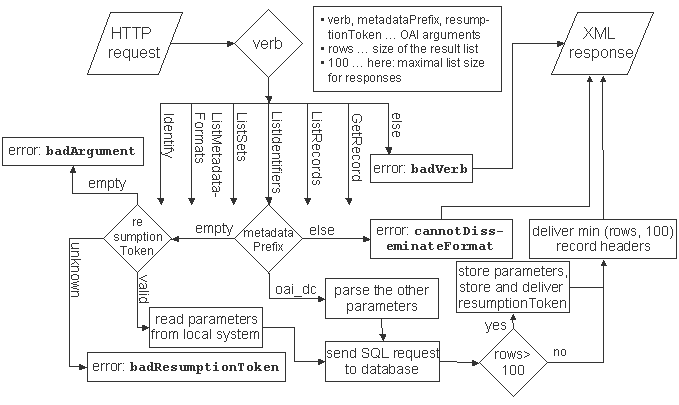
\includegraphics[scale=.15]{fig/oai_flow}
	\caption{Diagrama de flujo del servidor \acrshort{oaipmh}}\label{fig:oaiflow}
\end{figure}

El protocolo \acrshort{oaipmh} se basa en una arquitectura cliente-servidor en la que el cliente realiza las consultas por medio de transacciones \acrshort{http} GET o POST constituidas por un conjunto de opciones del tipo clave=valor. El servidor responde a la petición devolviendo un documento \acrshort{xml} bajo al menos el estandar \acrfull{dc}, según dicta la especificación de la implementación mínima del protocolo \acrshort{oaipmh} para los proveedores de información.\cite{OAIPMH_implementers}

Como se ve en la figura \ref{fig:oaiflow}\cite{oai_implementation} el cliente puede realizar seis peticiones al servidor en función del valor especificado en el `verb' de la consulta, las peticiones pueden ser:

\begin{itemize}
	\item \textbf{Idenfity:} Envía información sobre el servidor, así como el nombre del repositorio, \acrshort{url} base, correo electrónico del administrador del servidor, etc.
	\item \textbf{ListMetadataFormats:} Envía la lista de formatos en los que se encuentran disponibles los metadatos que al menos deben estar disponibles en \acrshort{dc}.
	\item \textbf{ListSets:} Envía una lista con los términos opcionales creados por el servidor para facilitar la recuperación de metadatos selectiva de los registros, posibilitando que un cliente pueda solicitar los registros pertenecientes a una clase en concreto. Estos términos representan una clasificación de los recursos según varias entradas. Los sets pueden estar compuestos por listas simple o formar una jerarquía.
	\item \textbf{ListIdentifiers: } Devuelve la cabecera de hasta un máximo de 100 registros por petición. Los identificadores pueden filtrarse por un rango entre dos fechas de creación o modificación o por los distintos ``sets'' definidos por el servidor.
	\item \textbf{ListRecords: } Realiza la misma tarea que la petición \textit{ListIdentifiers} a excepción de devolver el registro completo con sus metadatos, en lugar de incluir solo la cabecera del recurso. En caso de que la petición resulte una lista de más de 100 recursos, al igual que en la petición \textit{ListIdentifiers}, al final de la lista \acrshort{xml} se devolverá una clave `resumptionToken' que deberá ser utilizada por el cliente para continuar la devolución de los siguientes 100 registros en otra petición \acrshort{http} independiente.
	\item \textbf{GetRecord: } Petición utilizada para devolver un registro en concreto, siendo necesario especificar el identificador del recurso solicitado y el formato bibliográfico en el que se desea que se devuelva.
\end{itemize}

\clearpage

\lstinputlisting[language=XML, frame=single, label={lst:oaipmhgetrecord}, caption=Ejemplo de petición GetRecord de \acrshort{oaipmh}]{content/code/xml/get-record-example.xml}

El \acrshort{xml} generado por el servidor presenta la siguiente estructura para la extracción de los recursos:

\begin{itemize}
	\item \textbf{Información sobre la transacción:} El comienzo del \acrshort{xml} siempre está compuesto por atributos \textit{smlns}, \textit{smlns:xsi} y \textit{xsi:schemaLocation} que sirven para definir ``namespace'' y el esquema de \acrshort{oaipmh} del \acrshort{xml}.

	\item \textbf{La petición en cuestión:} En esta parte del \acrshort{xml} trata la información sobre una de las seis posibles peticiones. En el caso del GetRecords (véase algoritmo \ref{lst:oaipmhgetrecord}) por ejemplo, puede observarse que se compone de un elemento ``record'' y en el se subdivide en:
		\begin{itemize}
			\item Cabecera, en la que se especifica el identificador único, la fecha de creación o última modificación y la lista de ``sets'' a la que pertenece.
			\item Metadatos, la información misma del registro en cuestión compuesto por atributos tales como \textit{dc:title}, \textit{dc:creator}, \textit{dc:subjet}, y en general cualquiera de los atributos definidos en el set de elementos de \acrshort{dc}\cite{DCElements} o el formato bibliográfico que se haya especificado en la consulta.
		\end{itemize}
\end{itemize}
\section{Fortalezas y debilidades de las tecnologías}
\chapter{Objetivos del proyecto}

\section{Definición del proyecto}

\subsection{Objetivos}

La gestión de repositorios semánticos compatibles con el estándar \acrshort{oaipmh} tiene como objetivo explotar la información almacenada en un repositorio de manera más eficiente, mediante consultas semánticas y facetadas avanzadas. Busca dar soporte a \acrshort{oaipmh} para disponer de todo el contenido según dicta su estándar.

Como caso práctico se propone añadir compatibilidad con \acrshort{oaipmh} al sistema de gestión de grupos de investigación LabMan, para que pueda proveer de datos a clientes que trabajen con esta tecnología.

Para dar sentido a esta funcionalidad, se pretende expandir labman con un cliente que se alimente con estos recursos para ofrecer servicios orientados a la búsqueda semántica y facetada.
\subsection{Alcance del proyecto}

Atendiendo a las premisas señaladas anteriormente, las funcionalidades que deberá soportar este proyecto serán:

\begin{itemize}
	\item Un servidor capaz de conectarse al repositorio de \acrshort{labman} y extraer la información actualizada, en forma de metadatos, sobre las publicaciones y sus autores correspondientes de acuerdo con el estándar \acrlong{dc}\cite{DC}, respondiendo a las peticiones \acrshort{http} de acuerdo con el protocolo \acrshort{oaipmh}.
	
	\item Un cliente web que extienda \acrshort{labman} capaz de realizar busquedas y filtros complejos sobre los proyectos y publicaciones mediante un proceso intuitivo para los usuarios, compuesto por formularios que se dispondrán de forma sencilla en primera instancia, para dar la posibilidad de realizar consultas rápidas y simples sin abrumar a los usuarios por la longitud del mismo. Pero, a su vez, han de permitir dar la posibilidad de expandir los campos con el fin de introducir datos más específicos para realizar consultas más elaboradas.

	\item La plataforma estará diseñada de una manera intuitiva, para que así, personas con pocos conocimientos de la informática también la puedan usar sin ningún tipo de problema. Además ha de ser responsiva, es decir, su diseño se adaptará a distintos tamaños de pantallas como pueden ser las de un ordenador de sobremesa, un portátil, una tableta o un móvil, donde poder plasmar toda la información de una manera legible para los humanos.
\end{itemize}
\subsection{Producto final}

El producto final se compone de dos sistemas diferentes:

El primero es un servidor de documentos \acrfull{xml}\cite{XML} en el esquema \acrshort{dc}, capaz de responder a las peticiones \acrshort{html} según el protocolo \acrshort{oaipmh}. Será capaz de proveer información variada acerca de las publicaciones de los miembros que conforman MORElab en DeustoTech.

Los datos que proporcionará serán una relación de las tablas del repositorio de \acrshort{labman} acerca de las publicaciones pudiendo ser:

\begin{itemize}
	\item Actas.
	\item Ponencias.
	\item Tesis doctorales.
	\item Artículos de revistas.
	\item Artículos de publicaciones.
	\item Libros.

\end{itemize}

La segunda es una aplicación web que permita a todo el mundo consultar y filtrar la información, de forma esquematizada y ordenada, sobre las publicaciones y proyectos del equipo de investigación de MORElab por medio de sus atributos más significativos a través de formularios dinámicos e interactivos.

\section{Descripción de realización}

\subsection{Método de desarrollo}

El proyecto se desarrollará mediante un sistema de fases, en las que el orden es algo vital puesto que cada una de las fases dependerá de la previa, en el \acrfull{edt} (figura \ref{fig:edt}) puede verse su estructura.

\begin{figure}[!htp]
	\centering
	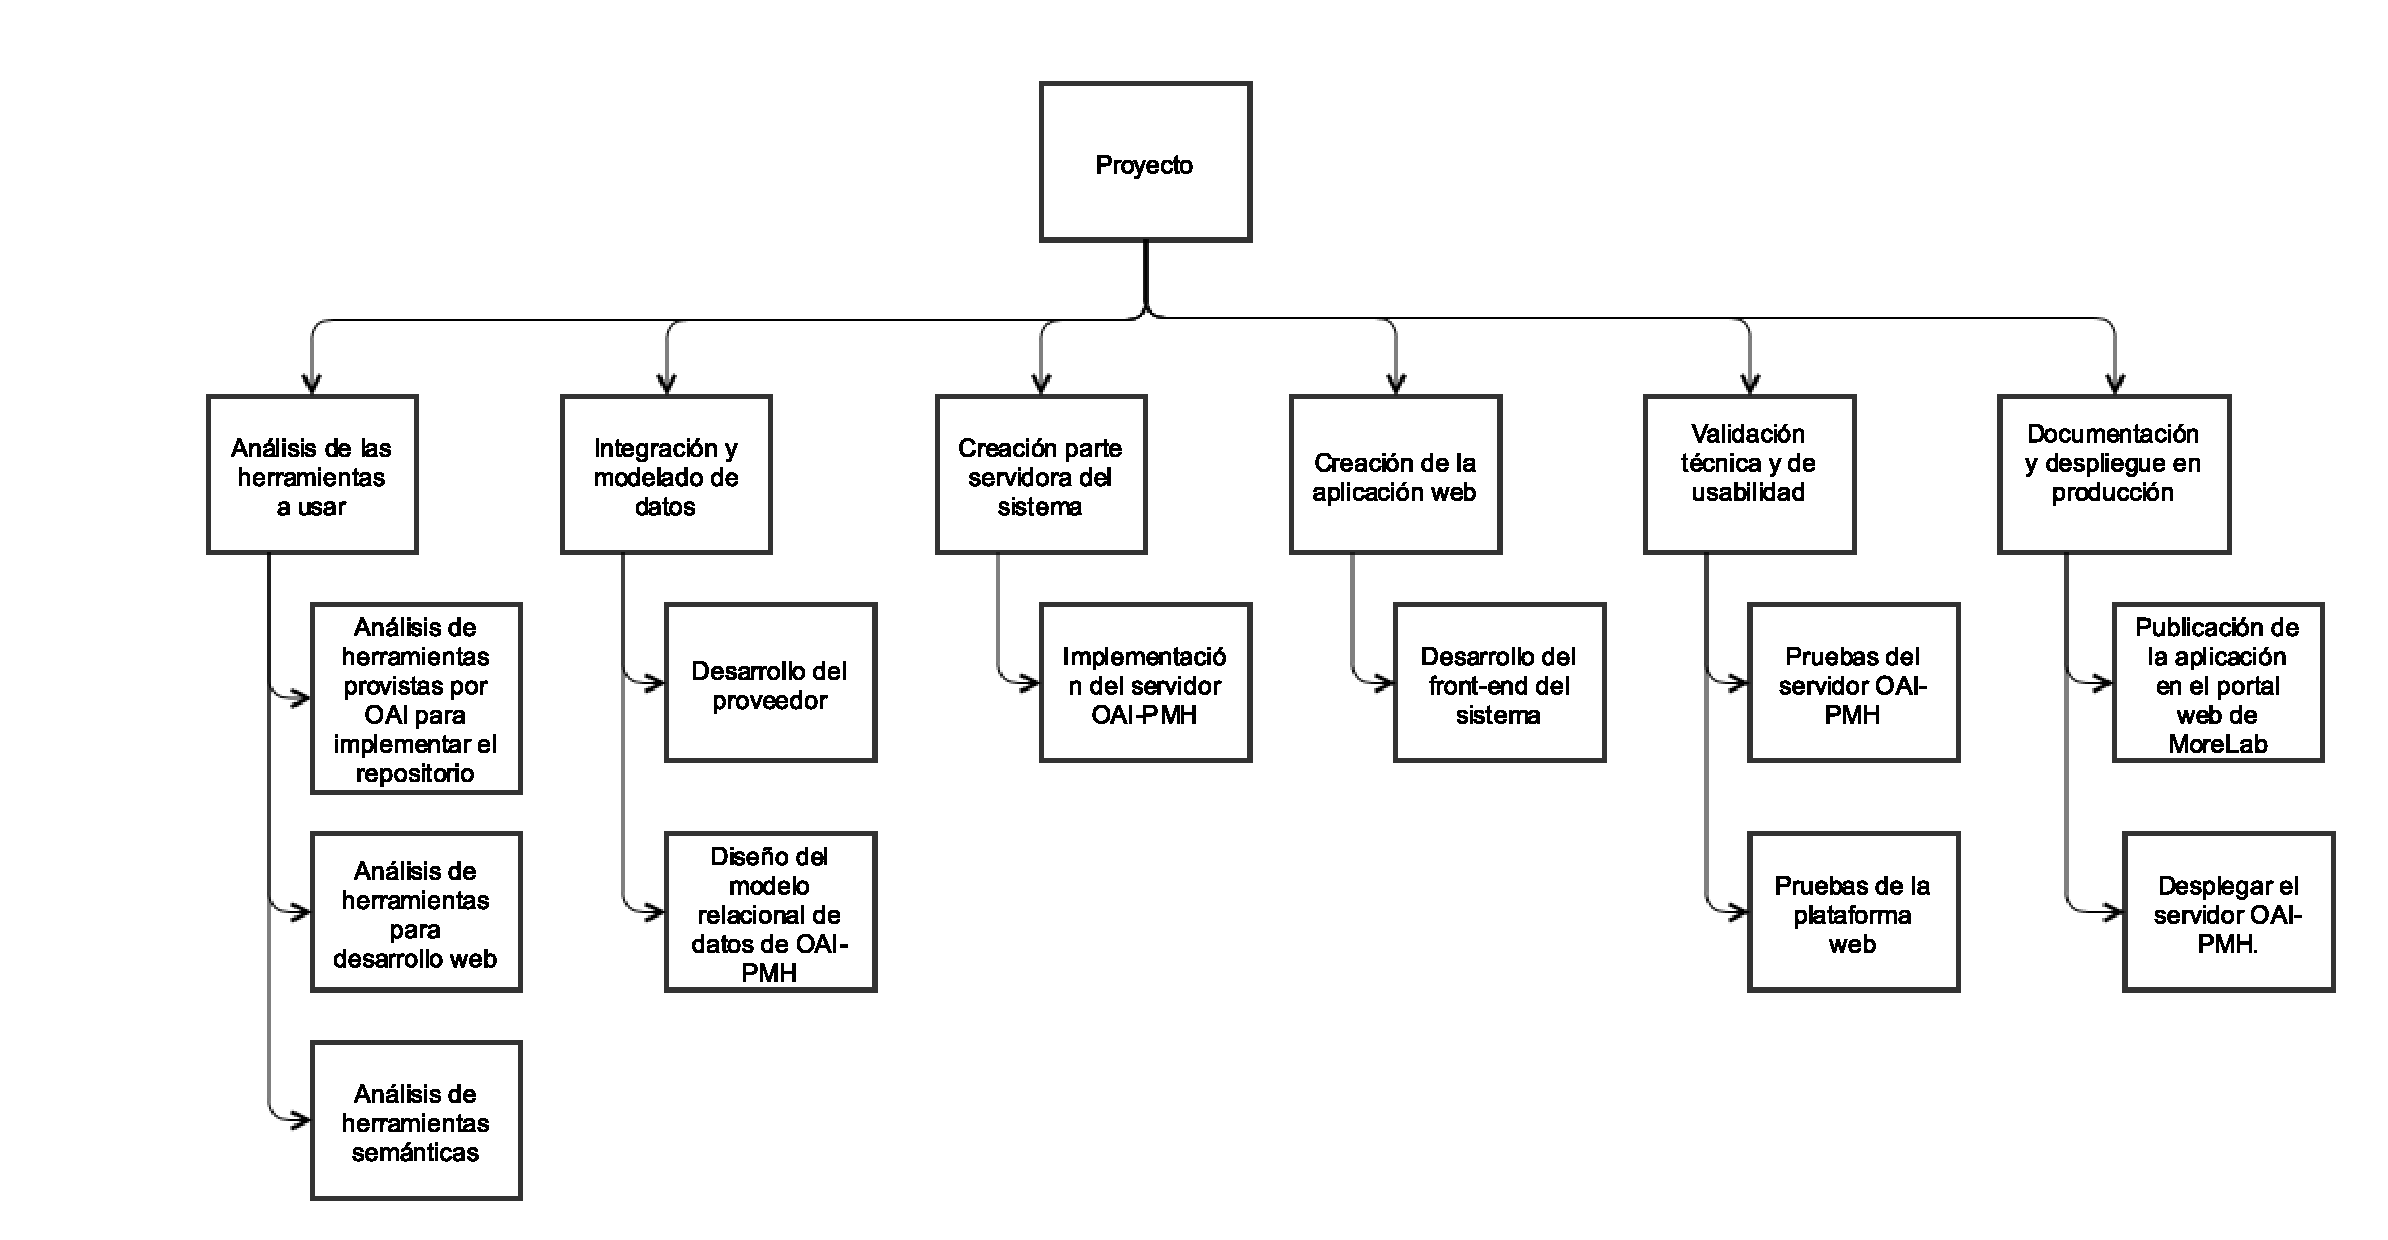
\includegraphics[angle=-90, scale=.5]{fig/edt}
	\caption{EDT}\label{fig:edt}
\end{figure}

Por tanto, las fases de la solución planteada serán las siguientes:

\begin{enumerate}
	\item \textbf{Análisis de las herramientas a usar:}

	En esta fase se analizarán todas las posibles herramientas que se pueden usar para el desarrollo del proyecto y se elegirán las más adecuadas de acuerdo a las necesidades del proyecto y a los conocimientos del equipo de trabajo.
	\item \textbf{Integración y modelado de datos:}

	Es la fase en la que se identificará y seleccionarán las tablas del repositorio de las que se extraerá la información para su adaptación a Dublin Core.
	\item \textbf{Creación del servidor de OAI-PMH:}

	Diseño e implementación servidor.
	\item \textbf{Creación de la aplicación web:}

	Diseño e implementación del front-end de la aplicación web. 
	\item \textbf{Validación técnica y de usabilidad:}

	Es la fase donde se realizarán las pruebas finales del sistema completo.
	\item \textbf{Documentación y despliegue en producción:}

	Es donde se terminará de redactar la documentación necesaria y se desplegará el producto.
\end{enumerate}
\subsection{Productos intermedios}

Los productos intermedios que se generarán en cada una de las fases son:

\begin{itemize}
	\item \textbf{Integración y modelado de datos:}
	\begin{itemize}
		\item Especificación y diseño de la base de conocimiento del servidor \acrshort{oaipmh}.
	\end{itemize}
	\item \textbf{Creación parte servidora del sistema:}
	\begin{itemize}
		\item Módulo de proveedor de la base de conocimiento.
		\item Módulo de adaptación y almacenamiento del conocimiento en \acrlong{dc}.
		\item Módulo de servicio de \acrshort{xml}.
	\end{itemize}
	\item \textbf{Creación de la aplicación web:}
	\begin{itemize}
		\item Aplicación web del sistema.
	\end{itemize}
	\item \textbf{Validación técnica y de usabilidad:}
	\begin{itemize}
		\item Informe de evaluación del sistema.
	\end{itemize}
\end{itemize}
\subsection{Tareas principales}

La implantación del proyecto comprende las siguientes tareas o actividades: 

\subsubsection{Análisis de las herramientas a usar:}

\begin{itemize}
	\item \textbf{Análisis de herramientas provistas por \acrshort{oai} para implementar los requisitos mínimos para repositorio del protocolo \acrshort{oaipmh}.}

	Investigar las distintas alternativas que hay para crear un servidor que beba de distintos tipos repositorios.
	\item \textbf{Análisis de herramientas para desarrollo web.}

	Investigar las distintas herramientas que hay para el desarrollo web y que sean adecuadas para el propósito del proyecto.
	\item \textbf{Análisis de herramientas semánticas.}

	Investigar las distintas alternativas para realizar búsquedas según los estándares de la web semántica. 
\end{itemize}

\subsubsection{Integración y modelado de datos:}

\begin{itemize}
	\item \textbf{Desarrollo del proveedor.}
	
	Desarrollo del sistema de extracción de datos de las tablas necesarias del repositorio PostgreSQL.

	\begin{enumerate}
		\item Formación: aprendizaje en el uso de las herramientas.
		\item Diseño: diseño del sistema de extracción de datos.
		\item Implementación: programación del sistema de extracción de datos.
		\item Pruebas: pruebas del sistema de extracción de datos.
	\end{enumerate}
	\item \textbf{Diseño del modelo relacional de datos de \acrshort{oaipmh}.}
	\begin{enumerate}
		\item Diseño: diseño del modelo de la base de datos. 
		\item Implementación: inserción del modelo de datos en la base de datos.
		\item Pruebas: pruebas de la base de datos junto con el sistema de extracción de datos.
	\end{enumerate}
\end{itemize}

\subsubsection{Creación parte servidora del sistema:}

\begin{itemize}
	\item Implementación del servidor \acrshort{oaipmh}.

	Puesta en marcha del servidor \acrshort{oaipmh} que transforma datos almacenados mediante un modelo relacional a \acrshort{dc}.

	\begin{enumerate}
		\item Implementación: configuración del servidor.
		\item Pruebas: pruebas del servidor.
	\end{enumerate}
\end{itemize}

\subsubsection{Creación de la aplicación web:}

\begin{itemize}
	\item \textbf{Desarrollo del front-end del sistema.}
	\begin{enumerate}
		\item Formación en la herramienta de desarrollo web.
		\item Diseño básico de la plataforma web.
		\item Diseño del módulo de búsqueda avanzada de proyectos.
		\item Diseño del módulo de búsqueda avanzada de publicaciones.
	\end{enumerate}	
\end{itemize}

\subsubsection{Validación técnica y de usabilidad:}

\begin{itemize}
	\item \textbf{Pruebas del servidor \acrshort{oaipmh}.}
	\item \textbf{Pruebas de la plataforma web.}
\end{itemize}

\subsubsection{Documentación y despliegue en producción:}

\begin{itemize}
	\item \textbf{Publicación de la aplicación en el portal web de MoreLab.}
	
	Instalar la aplicación web en el servidor de LabMan y publicarlo en el portal web.
	\item \textbf{Desplegar el servidor \acrshort{oaipmh}.}

	Instalar el servidor \acrshort{oaipmh}, recolectar y exportar la información del repositorio.
\end{itemize}

\clearpage

\section{Organización y equipo}

\subsection{Esquema organizativo}

La organización del proyecto se articula en torno al comité de dirección y al equipo de trabajo que se va a encargar de desarrollar el producto, en función de la estructura de la figura \ref{fig:org_schema}.

\begin{itemize}
	\item \textbf{Comité de dirección:} su función principal es orientar por dónde debería ir el proyecto y tomar las decisiones finales a la hora de qué hacer o no. Además, este comité deberá aprobar las diferentes fases del proyecto.
	\item \textbf{Equipo de trabajo:} el órgano encargado de diseñar y desarrollar el contenido del proyecto en función de las diferentes fases estipuladas.
	\item \textbf{Seguimiento:} Debido a el bajo número de personas que compone el equipo de desarrollo se ha acordado trabajar mediante reuniones de seguimiento semanales pero también tras terminar cada tarea. En las reuniones semanales se reunirán todos los miembros del equipo, mientras que en las que corresponden a una tarea finalizada lo harán solo los que han participado en dicha tarea junto a el director de proyecto. Su finalidad será comentar los avances y/o problemas que hayan podido ocurrir, aunque también servirán para que el director de el visto bueno a la tarea y pasar a la siguiente. 
\end{itemize}

\begin{figure}[!htp]
	\centering
	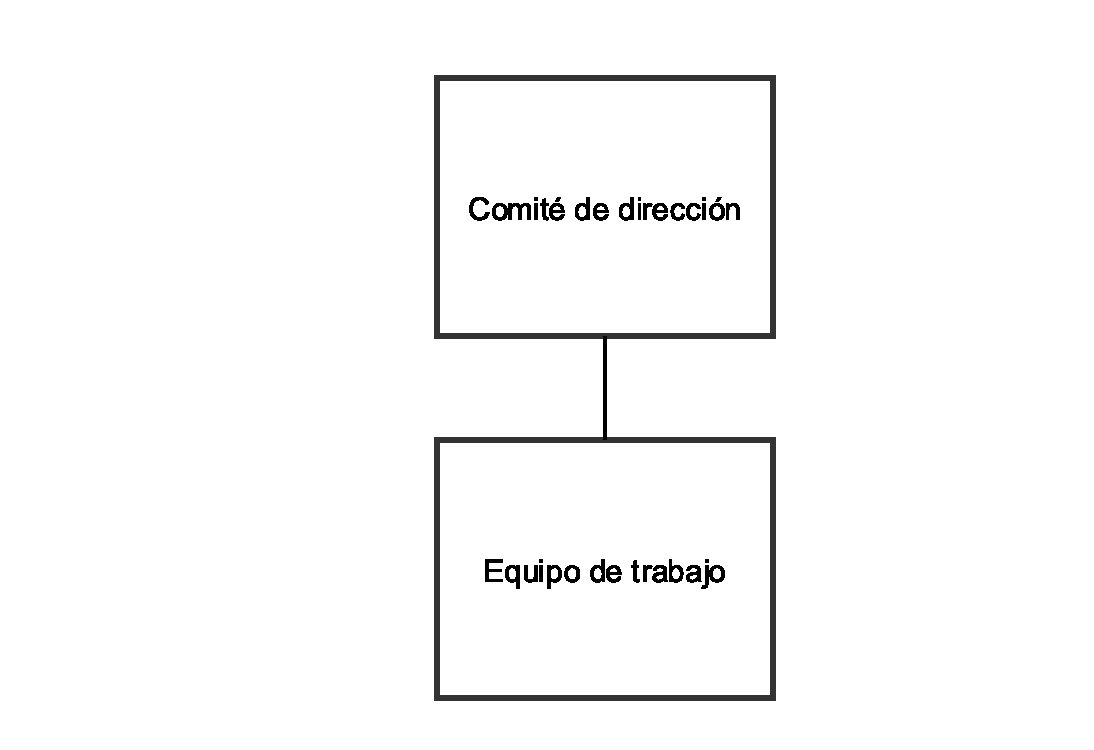
\includegraphics[scale=.75]{fig/organization}
	\caption{Esquema organizativo}\label{fig:org_schema}
\end{figure}
\subsection{Plan de Recursos Humanos}\label{sec:planRecursosHumanos}

El equipo de trabajo estará formado por los siguientes perfiles directamente relacionados con las diferentes áreas de competencias que se abordan en el proyecto: 

\begin{itemize}
	\item \textbf{Jefe de proyecto:} su función es realizar las actividades de organización, coordinación y seguimiento del proyecto.
	\item \textbf{Administrador de \acrlong{bd}}: su función es la de gestionar de una manera óptima la base de datos PostgreSQL y SPARQL además de colaborar en el estudio sobre las ventajas e inconvenientes tres tecnologías \acrshort{sql}, \acrshort{sparql} y acrshort{oaipmh}. 
	\item \textbf{Programador:} su función es la desarrollar toda la lógica del programa como la implementación de la plataforma web. 
	\item \textbf{Diseñador:} su función es la diseñar interfaces intuitivas para el usuario y adaptables para distintos dispositivos (portátiles, tablets, móviles) 
	\item \textbf{Experto en web semántica:} su función es ayudar en las cuestiones sobre la implementación de \acrshort{labman} relacionadas con la web semántica y colaborar en el estudio sobre las ventajas e inconvenientes tres tecnologías \acrshort{sql}, \acrshort{sparql} y acrshort{oaipmh}.
\end{itemize}

\section{Condiciones de ejecución}

\subsection{Entorno de trabajo}

El lugar de trabajo habitual serán las instalaciones de DeustoTech, aunque también se trabajará en casa para poder terminar a tiempo el proyecto.

El calendario y horario serán los correspondientes a los lugares de trabajo anteriormente mencionados durante una jornada laboral de aproximadamente 4 horas al día. Este horario podría verse modificado si se requiriera con el fin de cumplir los plazos establecidos.

En principio el director de proyecto será el responsable de todos los productos del desarrollo, y deberá dar el visto bueno a las herramientas que serán utilizadas para preservar las copias de seguridad y de definir cada cuanto tiempo deberán hacerse. En caso de que los desarrolladores no cumplan con estos requisitos y de producirse una perdida en el desarrollo serán estos los que asuman la responsabilidad, teniendo que optar por realizar horas extra o asumir de su sueldo la penalización que llegase a imponer el cliente en caso de no poder cumplirse con los plazos.

Los medios informáticos para la ejecución del proyecto deberán ser provistos por DeustoTech o serán los ordenadores personales de los integrantes del equipo. DeustoTech será responsable de todos los productos provistos para el desarrollo, salvo de aquellos medios pertenecientes a los propios desarrolladores. Los medios son los siguientes: 

\begin{itemize}
	\item Hardware
	\begin{itemize}
		\item Macbook Pro Retina 2012
		\item Servidor del repositorio Linux
		\item Monitor secundario
	\end{itemize}
	\item Software
	\begin{itemize}
		\item Licencia Sublime Text 2
		\item OS X
		\item Office 2011
		\item PostgreSQL
		\item SPARQL
	\end{itemize}
\end{itemize}
\subsection{Control de cambios}

Todas las peticiones que impliquen cambios en el diseño o en lo que ya está desarrollado, serán estudiadas y solo seguirán adelante si son modificaciones razonables y que son posibles de hacer dentro del plazo acordado. El procedimiento que habrá que seguir a la hora de  solicitar un cambio será:

\begin{enumerate}
	\item Comunicación de DeustoTech de las modificaciones solicitadas.
	\item Valoración por el equipo del proyecto de la repercusión técnica y cambios de plazos.
	\item Presentación de la decisión tomada por el equipo a DeustoTech.
	\item Notificación por parte de DeustoTech de la aprobación o no de la propuesta.	
	\item En caso afirmativo, modificación del plan de trabajo y del presupuesto.
\end{enumerate}
\subsection{Recepción de productos}

Para la recepción de productos, el equipo del proyecto definirá una serie de pruebas que serán estrictamente ejecutadas. Una vez pasadas las pruebas, el jefe de proyecto deberá revisar y aceptar el producto para poder presentarlo oficialmente a DeustoTech.  En caso de que exista algún problema tras la revisión,  la dirección de DeustoTech-Internet deberá comunicarlo en un plazo máximo de 5 días para poder llevar a cabo las modificaciones y así poder seguir con la siguiente fase del proyecto. En caso de no obtener respuesta en el intervalo de tiempo especificado anteriormente, se considerará aprobado.

\section{Planificación}

En esta sección se exponen los diversos aspectos relacionados con la planificación del proyecto. Para facilitar la compresión de los datos y figuras que se van a mostrar más adelante, en la tabla \ref{tab:task_id_name}, se expone la relación entre los identificadores de las tareas y sus denominaciones.

\begin{table}[htp]
	\centering
	\caption{Relación identificador-tarea}\label{tab:task_id_name}
	\begin{tabular}{cc}
		\toprule
    	\textbf{Identificador} & \emph{Nombre}\\
    	\midrule
    	T1 & Análisis de herramientas provistas por \acrshort{oai} para implementar el repositorio\\
    	T2 & Análisis de herramientas para desarrollo web\\
    	T3 & Análisis de herramientas semánticas\\
    	T4 & Desarrollo del proveedor\\
    	T5 & Diseño del modelo relacional de datos de \acrshort{oaipmh}\\
    	T6 & Implementación del servidor \acrshort{oaipmh}\\
    	T7 & Desarrollo del front-end del sistema\\
    	T8 & Pruebas del servidor \acrshort{oaipmh}\\
    	T9 & Pruebas de la plataforma web\\
    	T10 & Publicación de la aplicación en el portal web de MORElab\\
    	T11 & Desplegar el servidor \acrshort{oaipmh}\\
    	\bottomrule
    \end{tabular}
\end{table}

\subsection{Diagrama de precedencias}

En esta sección se muestra el diagrama de precedencias (ver figura \ref{fig:network_diagram}).

\begin{figure}[!htbp]
	\centering
	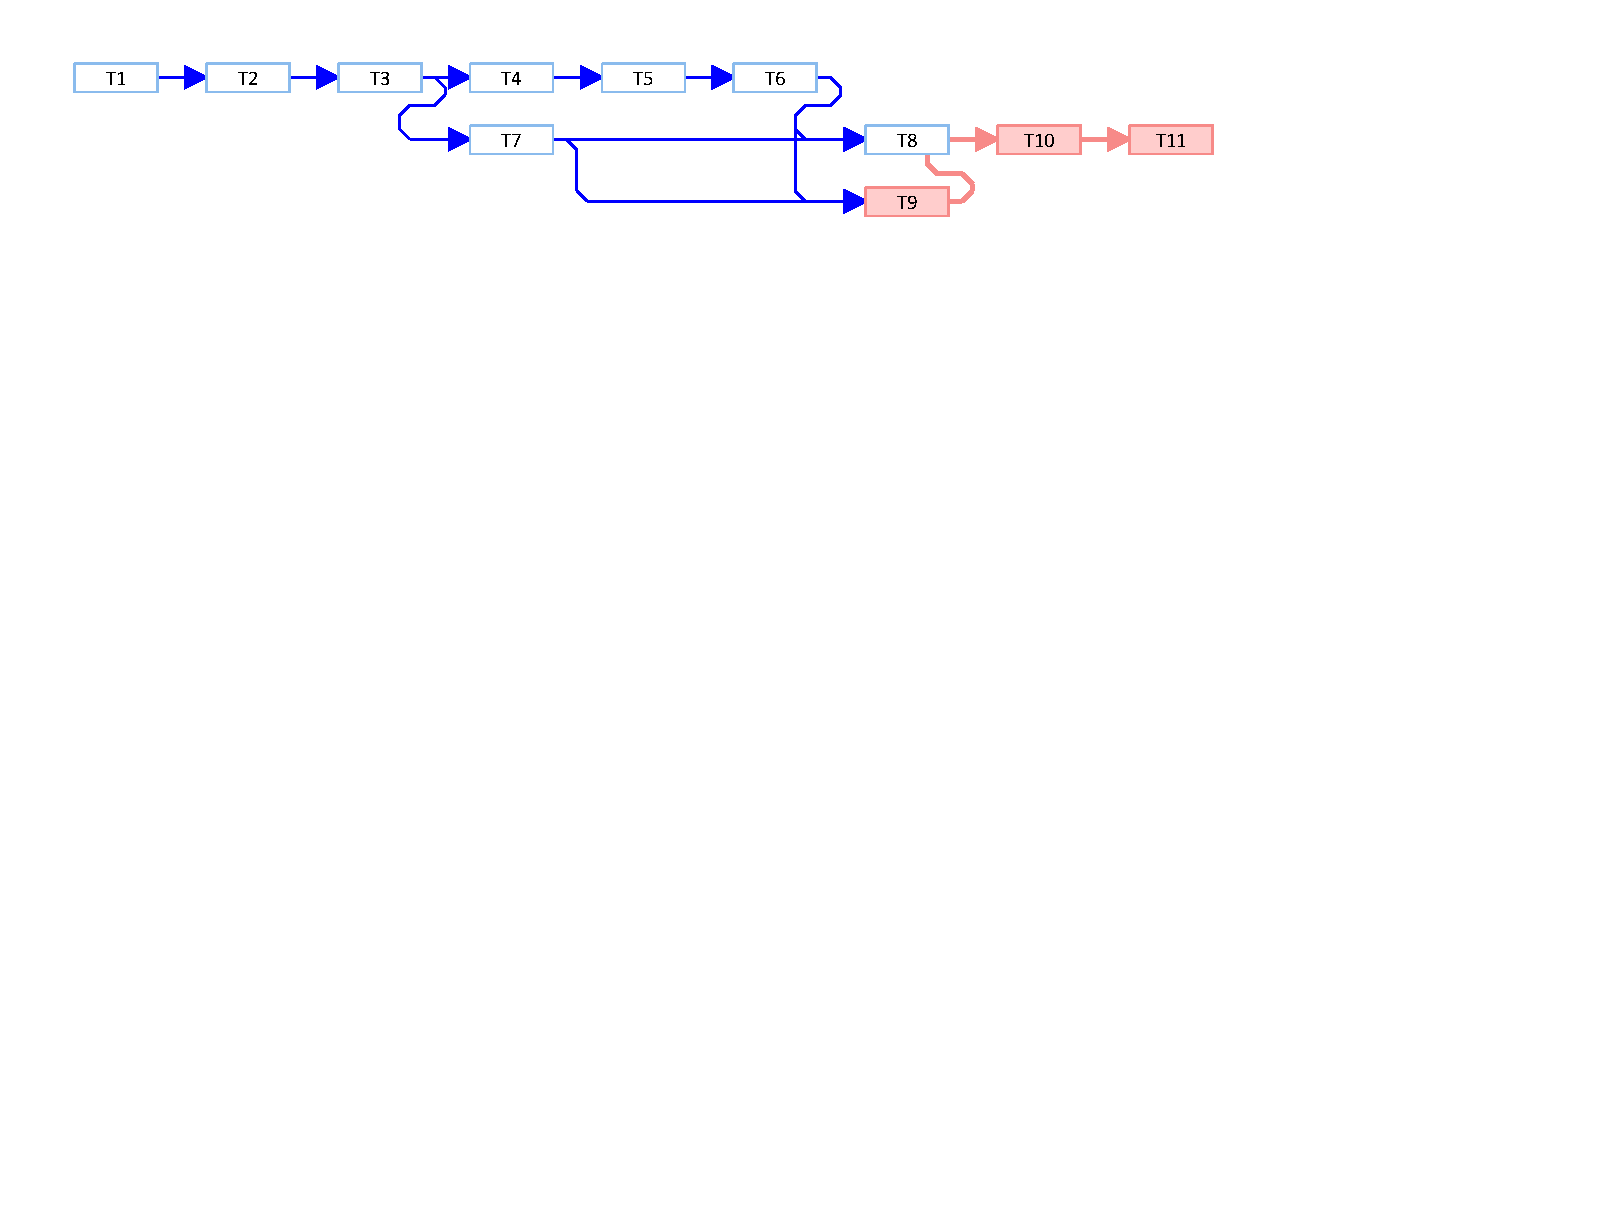
\includegraphics[page=1, scale=.65]{fig/network_diagram_simplified}
	\caption{Diagrama de precedencias}\label{fig:network_diagram}
\end{figure}

\begin{figure}[!htbp]
    \centering
    \includegraphics[page=2, scale=.65]{fig/network_diagram_simplified}
    \caption{Leyenda del diagrama de precedencias}
\end{figure}
\subsection{Plan de Trabajo}

En la tabla \ref{tab:work_plan} se especifica el plan de trabajo planificado.

\begin{table}[htp]
	\centering
	\caption{Presupuesto de Recursos Humanos}\label{tab:work_plan}
	\begin{tabular}{ccccccc}
		\toprule
    	\textbf{Nombre de tarea} & \emph{Duración} & \emph{Comienzo} & \emph{Fin} & \emph{Nombres de los recursos} & \emph{Predecesoras} & \emph{Trabajo}\\
    	\midrule
    	Análisis de herramientas provistas por \acrshort{oai} para implementar el repositorio\\
    	Análisis de herramientas para desarrollo web\\
    	Análisis de herramientas semánticas\\
    	Desarrollo del proveedor\\
    	Diseño del modelo relacional de datos de \acrshort{oaipmh}\\
    	Implementación del servidor \acrshort{oaipmh}\\
    	Desarrollo del front-end del sistema\\
    	Pruebas del servidor \acrshort{oaipmh}\\
    	Pruebas de la plataforma web\\
    	Publicación de la aplicación en el portal web de MORElab\\
    	Desplegar el servidor \acrshort{oaipmh}\\
    	\bottomrule
    \end{tabular}
\end{table}
\subsection{Diagrama de Gantt}

\begin{figure}[!htp]
	\centering
	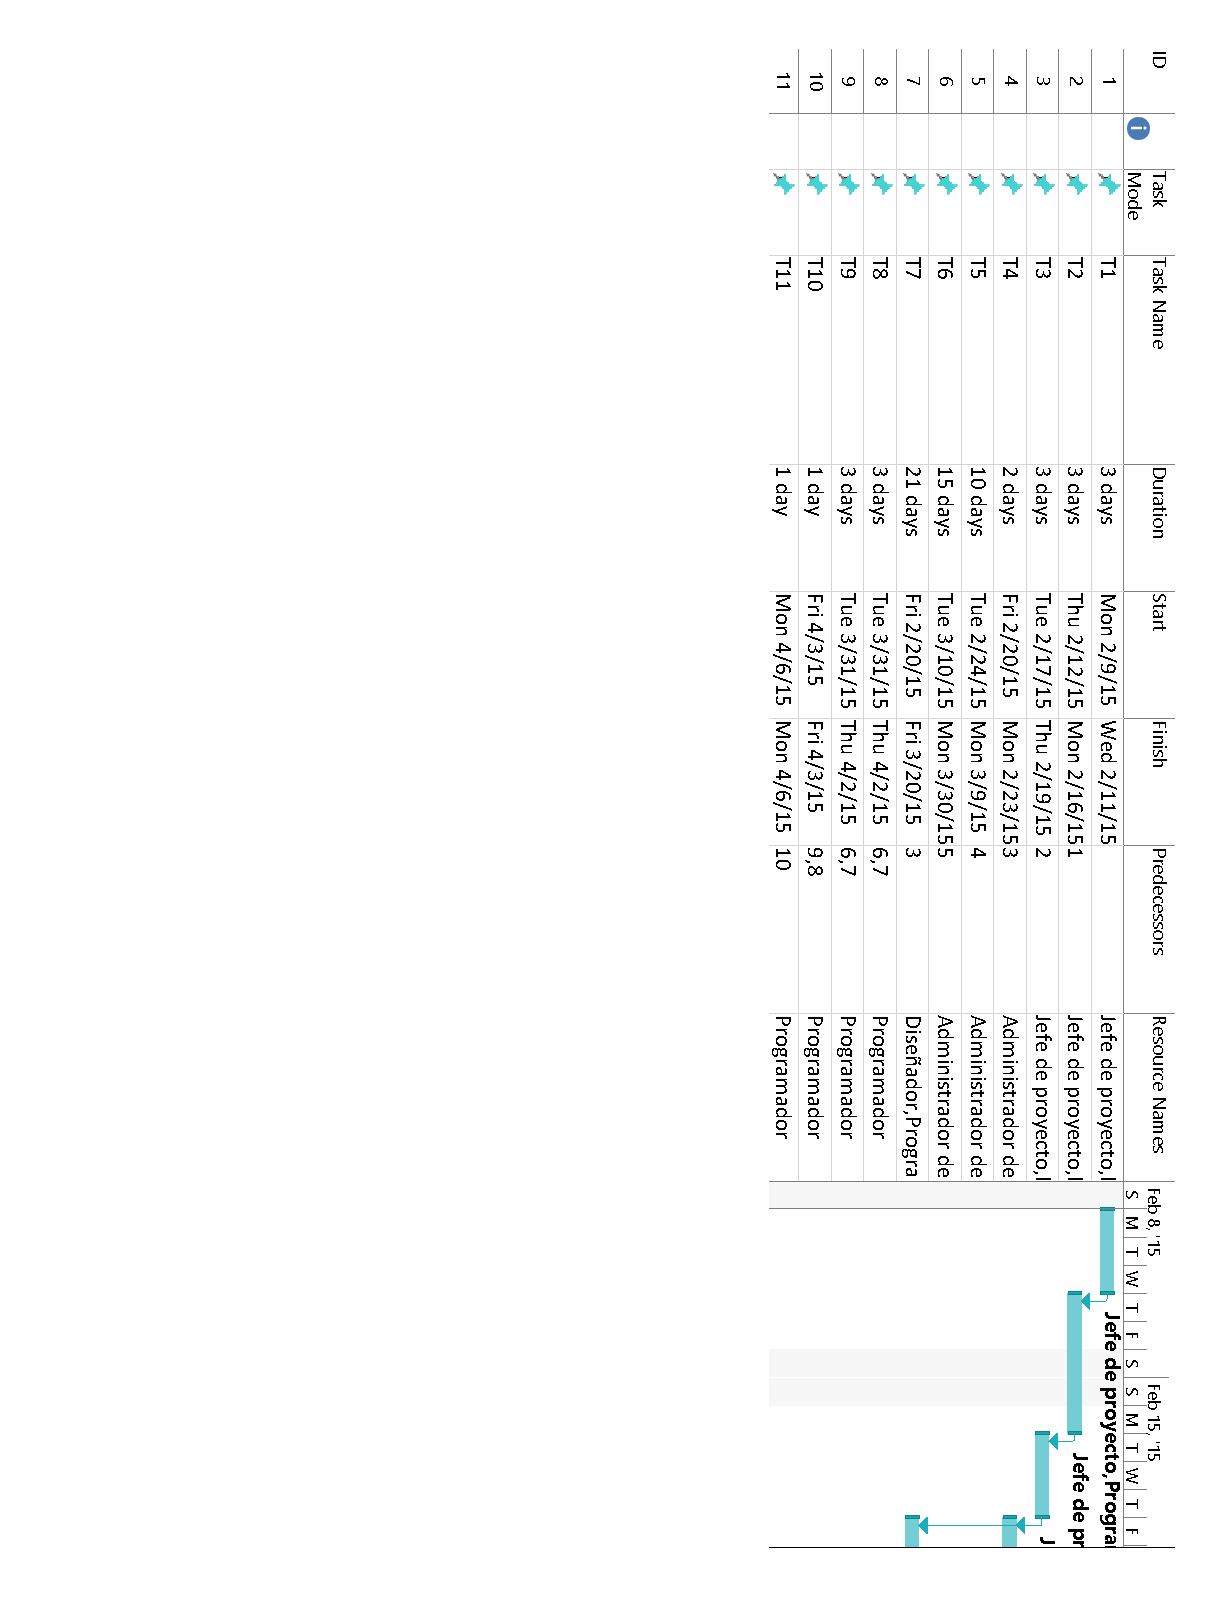
\includegraphics[page=1, scale=.7]{fig/gantt_diagram}
	\caption{Diagrama de Gantt 1}
\end{figure}

\begin{figure}[!htp]
	\centering
	\includegraphics[page=2, scale=.7]{fig/gantt_diagram}
	\caption{Diagrama de Gantt 2}
\end{figure}

\begin{figure}[!htp]
	\centering
	\includegraphics[page=3, scale=.7]{fig/gantt_diagram}
	\caption{Diagrama de Gantt 3}
\end{figure}

\begin{figure}[!htp]
	\centering
	\includegraphics[page=4, scale=.7]{fig/gantt_diagram}
	\caption{Leyenda del diagrama de Gantt}
\end{figure}
\subsection{Estimación de cargas de trabajo por perfil}

En esta sección se muestra la estimación de cargas de trabajo separado por los perfiles que existen en el proyecto (vease la tabla \ref{tab:workload})

\begin{table}[htp]
	\centering
	\caption{Cargas de trabajo por perfil}\label{tab:workload}
	\begin{tabular}{cc}
		\toprule
    	\textbf{Perfil de trabajo} & \emph{Carga de trabajo(h)}\\
    	\midrule
		Jefe de proyecto & 6,05\\
		Administrador de base datos & 64,05\\
		Diseñador gráfico & 26,22\\
		Experto en web semántica & 26,\\
		Programador & 185,48\\
    	\bottomrule
    \end{tabular}
\end{table}

\section{Presupuesto}

En esta sección se detalla el presupuesto planificado para la realización de proyecto. El presupuesto se desglosa en tres apartados diferentes: Recursos Humanos, Software y Hardware.

\subsection{Recursos Humanos}

En la tabla \ref{tab:budget-human} se detalla los honorarios por cada uno de los roles, dependiendo de las horas que trabaja según lo planificado.

\begin{table}[htp]
	\centering
	\caption{Presupuesto de Recursos Humanos}\label{tab:budget-human}
	\begin{tabular}{cccc}
		\toprule
    	\textbf{Rol} & \emph{Precio/hora(\euro/h)} & \emph{Carga de trabajo(h)} & \emph{Importe total(\euro)}\\
    	\midrule
    	Jefe de proyecto				&	40			&	6,05 					& 	242,00\\
		Administrador de base de datos	&	25			&	64,05					&	1.601,25\\
		Programador						&	25			&	185,48					&	4.637,00\\
		Diseñador						&	15			&	26,22					&	393,30\\
		Experto en web semántica		&	30			&	26,22					&	786,60\\
    	\bottomrule
    \end{tabular}
\end{table}
\subsection{Recursos software}

En la tabla \ref{tab:budget-software} se detalla el gasto destinado a las herramientas software según lo planificado.

\begin{table}[htp]
	\centering
	\caption{Presupuesto de software}\label{tab:budget-software}
	\begin{tabular}{cccc}
		\toprule
    	\textbf{Nombre} & \emph{Precio(\euro)} & \emph{Unidades} & \emph{Importe total(\euro)}\\
    	\midrule
    	Licencia Sublime Text 2		& 	70				&	1 			& 	70\\
    	Office 2011 				&	99				&	1			&	99\\
    	\bottomrule
    \end{tabular}
\end{table}
\section{Recursos Hardware}

\begin{table}[htp]
	\centering
	\caption{Presupuesto: Hardware}\label{tab:budget-hardware}
	\begin{tabular}{cccc}
		\toprule
    	\textbf{Nombre} & \emph{Precio(\euro)} & \emph{Unidades} & \emph{Importe total(\euro)}\\
    	\midrule
    	MBPR2012			& 	3.334			&	1 			&	3.334					\\
    	Monitor secundario	&	300				&	1			&	300						\\
    	\bottomrule
    \end{tabular}
\end{table}
\subsection{Total}

Para finalizar, en la tabla \ref{tab:total-budget} se detalla el presupuesto total, que se calcula mediante la suma del costo estimado de los Recursos Humanos, el Software y el Hardware.

\begin{table}[htp]
	\centering
	\caption{Presupuesto total}\label{tab:total-budget}
	\begin{tabular}{cc}
		\toprule
    	\textbf{Tipo} 		& 	\emph{Total}\\
    	\midrule
    	Recursos Humanos	& 			7.660,15\\
		Recursos Software	&			169,00\\
		Recursos Hardware	&			3.634,00\\
		\textbf{Total}		&	\textbf{11.463,15}\\
    	\bottomrule
    \end{tabular}
\end{table}
\chapter{Especificación de requisitos}
\chapter{Tecnologías utilizadas}

\section{Visión general}

En esta sección se presentan las diferentes tecnologías que se han utilizado para el desarrollo del proyecto. Las principales tecnologías usado son las siguientes:

\section{Servidor MOAI}

MOAI\cite{MOAI} es una plataforma capaz de recolectar información de diversas fuentes y publicarlas mediante el protocolo \acrshort{oaipmh} desarrollado por Infrae\cite{Infrae} con el fin de satisfacer las necesidades de las instituciones académicas que trabajan con metadatos relacionales y ficheros de información.

\begin{figure}[!htbp]
	\centering
	
\includegraphics{fig/moai_logo}
	\caption{Logotipo de MOAI}
\end{figure}

MOAI es una aplicación WSGI, implementado en Python, de ejecución local que requiere de un servidor \acrshort{http} como puede ser \acrshort{http} Apache\cite{HTTPApache} para servir su contenido en la red. MOAI incluye todas las funciones básicas como proveedor de datos del protocolo \acrshort{oaipmh}, indispensables para este proyecto. Por otra parte, permite tanto la extracción de la información de documentos \acrshort{xml} como recolectarla de diversos servidores de información tales como Fedora Commons\cite{Fedora}, EPrints\cite{EPrints} o DSpace\cite{DSpace} y almacenar la información cosechada en una base de datos SQLite\cite{SQLite} por defecto.

\subsection{Razón de uso}

Se ha escogido MOAI Server frete a las alternativas facilitadas por la misma comunidad de \acrshort{oai} en \url{https://www.openarchives.org/pmh/tools/tools.php} entre las que se cabe destacar a Fedora, EPrints y DSpace por las siguientes razones:

\begin{itemize}
	\item Su accesible documentación para el desarrollo y extensión del servidor.
	\item Capacidad para sobrescribir el esquema de la base de datos SQLite usado para la extracción de datos del servidor Apache por defecto y sustituirlo por la \acrshort{bd} PostgreSQL utilizada actualmente por LabMan, evitando replicar los datos.
	\item Implementado en una tecnología conocida, lo que reduce el tiempo de adaptación a la capa de datos.
\end{itemize}

\section{OAI-PMH validator}

\acrshort{oaipmh} validator\cite{oaipmh_validator} es una página web que permite validar el \acrshort{xml} generado por proveedores de datos de \acrshort{oaipmh} en desarrollo y comprobar si existe algún error en la estructura de la petición y si además realmente cumple con el estándar respetando el esquema \acrshort{oaipmh} y el formato bibliográfico \acrshort{dc}.


\begin{figure}[!htbp]
	\centering
	
\includegraphics[scale=0.5]{fig/oaipmh_validator_logo}
	\caption{Logotipo de \acrshort{oaipmh} validator}
\end{figure}

La aplicación web permite validar como descargar la petición resultante a partir de las \acrshortpl{url} de servidores públicos de forma gratuita, permitiendo realizar cinco de las seis operaciones que establece el protocolo \acrshort{oaipmh}. Además facilita la validación directa de fuentes \acrshort{xml} generados por servidores que aún están en pruebas y no son públicos también de forma gratuita. A modo de aclaración, en la figura \ref{fig:oai_validator} se muestra un ejemplo de una validación del comando \textit{ListMetadataFormats} mediante una consulta POST a el repositorio \url{https://dspace.lib.uom.gr/dspace-oai/request}.

\begin{figure}[!htbp]
	\centering
	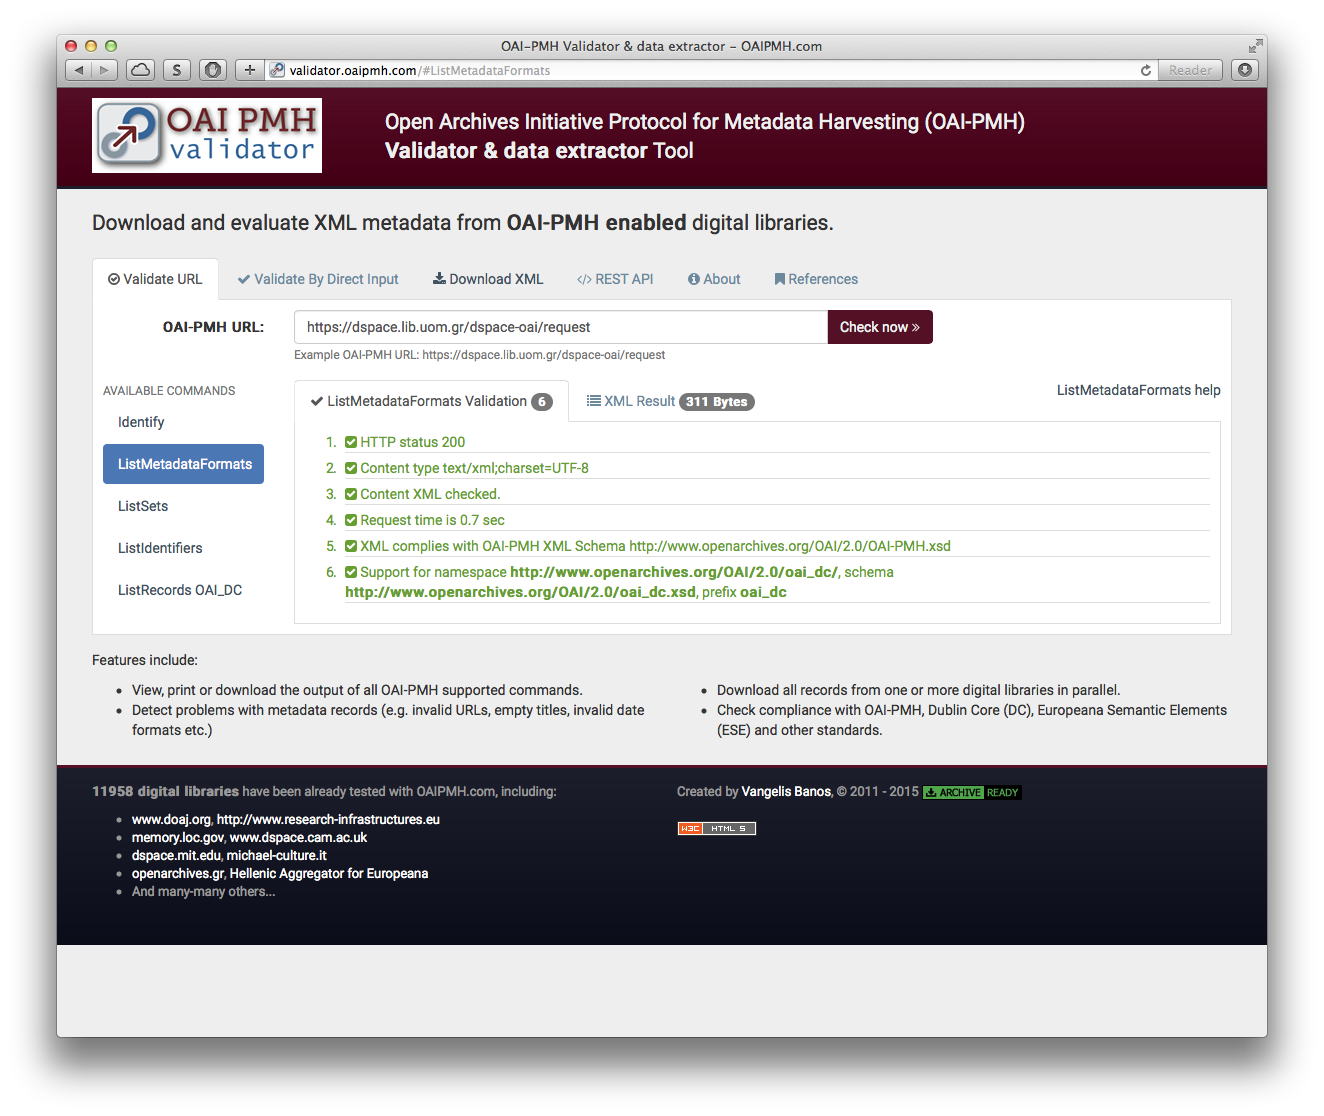
\includegraphics[scale=0.2]{fig/oaipmh_validator_example}
	\caption{Ejemplo de validación de una consulta en \acrshort{oaipmh} validator}
	\label{fig:oai_validator}
\end{figure}

\subsection{Razón de uso}

Se ha utilizado esta aplicación web frente a los distintos validadores existentes como Oval\cite{Oval}, principalmente por que ha permitido comprobar la velidez de los \acrshortpl{xml} generados por el proveedor de información, en la etapa de desarrollo en el que el servidor no era público y por tanto no disponía de una \acrshort{url} a la que hacer referencia para realizar dichas comprobaciones.

\section{SQLAlchemy}

SQLAlchemy\cite{SQLAlchemy} consiste tanto en \acrfull{orm} como en un juego de herramientas \acrshort{sql} para el lenguaje de programación Python. Como los propios desarrolladores definen ``SQLAlchemy ofrece una \textit{suite} completa de patrones de persistencia, diseñada para una acceso eficiente y de alto rendimiento a la \acrlong{bd}, adaptado a lenguaje sencillo como lo es Python''

\begin{figure}[!htbp]
	\centering
	
\includegraphics[scale=0.5]{fig/sqla_logo}
	\caption{Logotipo de SQLAlchemy}
\end{figure}

\subsection{Razón de uso}

Se ha utilizado esta \acrshort{api} frente a otras soluciones, como puede ser el \acrshort{orm} de Django, principalmente por las siguientes razones:

\begin{itemize}
	\item Ofrece un nivel de abstracción mayor manipulando las tablas de la \acrshort{bd} como si de objetos de Python se tratasen.
	\item Permite escoger el grado de abstracción deseado, pudiendo escoger entre las herramientas \textit{core}, para la manipulación de tablas, o del \acrshort{orm} para gestionar el propio modelo de la \acrshort{bd} como objetos.
	\item Es uno de los \acrshortpl{orm} más usados, utilizado por organizaciones como Mozilla\cite{Mozilla} o Reddit\cite{Reddit}.
	\item Ofrece una documentación detallada tanto para el uso de las herramientas \textit{core} como para aquellas relacionadas con el \acrshort{orm} en sí. Además debido a ser una de las herramientas más usadas dispone de una gran comunidad que está dispuesta a ayudar a resolver cualquier problema.
	\item Soporta desde Python 2.5 hasta las últimas versiones 3.x del mismo.
	\item SQLAlchemy incluye dialectos para \acrlongpl{bd} como SQLite, PostgreSQL, MySQL, Oracle\cite{Oracle}, MS-SQL\cite{MSSQL}, Firebird\cite{Firebird} y muchas otras por medio de extensiones, por lo que las clases generadas con esta herramienta pueden ser reutilizadas en caso de migración a una de estas \acrshort{bd}.
	\item Estaba integrado como una dependencia por el servidor de MOAI lo que evitaba los quebraderos de cabeza de tener que instalar otros \acrshortpl{orm}
\end{itemize}

\section{Django}

Django es un \textit{framework open-source} para el desarrollo de aplicaciones web escrito en Python y basado en el patrón \acrfull{mvc}. El principal objetivo de Django, es facilitar el proceso de creación de paginas web complejas enfatizando especialmente en la reusabilidad y en la modularidad de sus componentes bajo el lema inglés \acrfull{dry}.

\begin{figure}[!htbp]
	\centering
	
\includegraphics[scale=0.18]{fig/django_logo}
	\caption{Logotipo de Django}
\end{figure}

\subsection{Razón de uso}

Se ha utilizado este entorno de desarrollo frente a otras soluciones, como puede ser \acrfull{ror}\cite{RoR} o más modernas como Express\cite{Express} por las siguientes razones:

\begin{itemize}
	\item Es usado por grandes páginas como Mozilla, The Washington Times\cite{TWT} o Bitbucket\cite{Bitbucket}.
	\item El \acrshort{orm} de Django es una herramienta para la gestión de las \acrlongpl{bd} extremadamente potente, además de ser es una de las más usadas en la comunidad de Python.
	\item La interfaz de administración es muy potente y personalizable por lo que ahorra mucho tiempo de desarrollo.
	\item Contiene una serie de extensiones, como Graph models\cite{GraphModel} que ha facilitado el renderizado automatizado de los modelos relacionales que se presentan es este documento a partir de las clases de Python que definen a cada entidad.
	\item Principalmente por que \acrshort{labman} está desarrollado en esta tecnología y para extenderla se ha tenido que trabajar con ella para no desechar lo que ya estaba hecho.
\end{itemize}

\section{jQuery}

jQuery\cite{jQuery} es una librería multiplataforma gratuita de \acrfull{js} diseñada para simplificar el desarrollo de la parte cliente. La sintaxis de jQuery está pensada para facilitar la navegación por el árbol de elementos del \acrfull{dom}, proporcionando funciones para la manipulación de los mismos. El objetivo de jQuery es poder realizar todas las operaciones que se podría realizar con \acrshort{js} teniendo que escribir mucho menos código para conseguirlo.

\begin{figure}[!htbp]
	\centering
	\includegraphics[scale=0.6]{fig/jquery_logo}
	\caption{Logotipo de jQuery}
\end{figure}

\subsection{Razón de uso}

Se ha utilizado esta \acrshort{api} de \acrshort{js} frente a otras posibles soluciones, como puede Prototype\cite{Prototype} por las siguientes razones:

\begin{itemize}
	\item jQuery es una tecnología intuitiva, fácil de aprender que simplifica el código además del tiempo de desarrollo de la aplicación.
	\item Tiene una gran comunidad por detrás que crea infinitos tutoriales para ayudar a los desarrolladores novatos a dar sus primeros pasos.
	\item jQuery es una librería multiplataforma y compatible con todos los navegadores web que se encarga de solucionar los problemas de \acrshort{js} presentes en las primeras versiones de Firefox\cite{Firefox} o \acrfull{ie}\cite{IE}, permitiendo escribir el código una sola vez para todos los navegadores.
\end{itemize}

\section{Bootstrap}

Bootstrap en un \textit{framework} gratuito para la creación de aplicaciones web que contiene unas plantillas, basadas en \acrshort{html} y \acrshort{css}, para formularios, botones, navegación y muchos otros tipos de componentes de la interfaz gráfica, así como extensiones \acrshort{js}. El objetivo de Bootstrap es facilitar el desarrollo web ofreciendo la posibilidad de generar interfaces de usuario con aspecto visual atractivo sin la necesidad de disponer de nociones de diseño gráfico.

\begin{figure}[!htbp]
	\centering
	
\includegraphics[scale=0.45]{fig/bootstrap_logo}
	\caption{Logotipo de Bootstrap}
\end{figure}

Fue creado por dos desarrolladores en Twitter para fomentar la consistencia entre las herramientas internas y fue publicado como código abierto más adelante, convirtiéndose en uno de los \textit{framework} de desarrollo web más destacados.

Además, para complementar a Bootstrap se han utilizado las siguientes extensiones para resolver ciertos problemas en la consistencia del \textit{look and feel} de varios componentes y añadir nuevas funciones:

\subsection{Bootstrap-select}

Bootstrap-select\cite{BootstrapSelect} es una extensión que añade el estilo característico de Bootstrap las etiquetas \textit{select} de \acrshort{html}, sobrescribiendo el estilo dependiente del sistema operativo que disponen por defecto. 

Este \textit{plugin} no solo altera el aspecto visual del componente de selección, sino que, por otra parte añade la posibilidad disponer los elementos en agrupaciones, añadir validaciones como un máximo y mínimo de elementos seleccionados y facilitar la modificación del componente mediante \acrshort{js}.

\begin{figure}[!htbp]
	\centering
	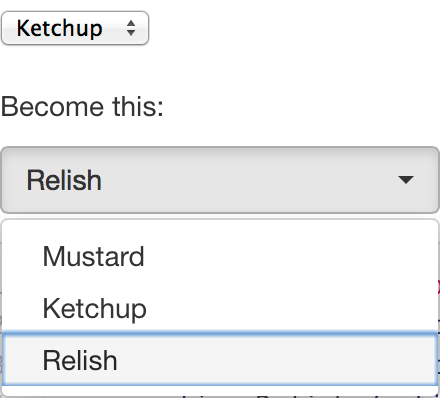
\includegraphics[scale=0.45]{fig/bootstrap_select}
	\caption{Cambio visual producido por Bootstrap-select}
	\label{fig:bootstrap-select}
\end{figure}

\FloatBarrier

En la figura \ref{fig:bootstrap-select} puede observarse el cambio visual que sufre el componente \text{select} renderizado bajo Safari\cite{Safari}.

\subsection{Bootstrap 3 Datepicker}

Bootstrap 3 Datepicker\cite{BootstrapDatepicker} es una extensión que combina varios elementos de Bootstrap y le añade la funcionabilidad de un \textit{input date} nativo de \acrshort{html}5 manteniendo así la armonía estética característica de Bootstrap.

\begin{figure}[!htbp]
	\centering
	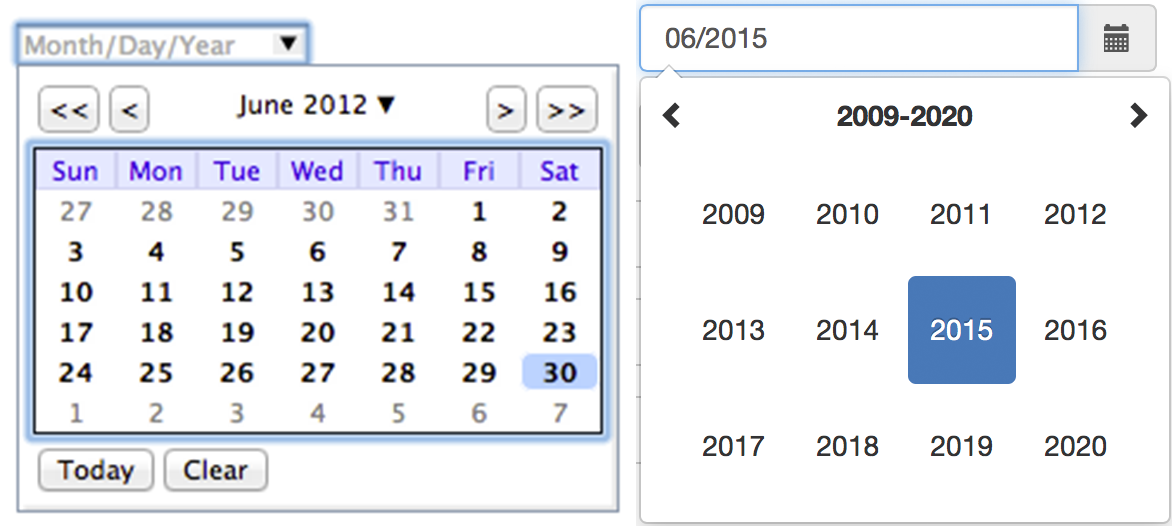
\includegraphics[scale=0.25]{fig/bootstrap_datepicker}
	\caption{Cambio visual producido Bootstrap 3 Datepicker}
	\label{fig:bootstrap-datepicker}
\end{figure}

Además de otorgar un cambio visual, tal y como puede observarse en la figura \ref{fig:bootstrap-datepicker}, esta \acrshort{api} aporta facilidades para la manipulación de los atributos de este componente, así como la gestión de eventos.

\subsection{Razón de uso}

Se ha utilizado este \textit{framework} para el diseño del \textit{front-end} frente a otras posibles soluciones, como puede Skeleton\cite{Skeleton} por las siguientes razones:

\begin{itemize}
	\item Aumenta la velocidad del desarrollo. Al facilitar el diseño de muchos de los componentes \acrshort{html} para formularios, tipográficas, etc. el desarrollador puede desentenderse de apartado artístico y dedicarse a la lógica de la aplicación web.
	\item A partir de la versión 2.0 de Bootstrap ofrece soporte responsivo, es decir, la capacidad para adaptarse a múltiples dispositivos, como pueden ser tabletas, equipos de sobremesa, dispositivos móviles, teniendo que desarrollar una única vez el apartado gráfico.
	\item El soporte, Bootstrap ha acumulado tras de sí una gran comunidad que está dispuesta a solucionar cualquier problema que pueda surgir durante el desarrollo de interfaces gráficas.
	\item Comunidad de desarrolladores artísticos, Bootstrap dispone miles de artistas que diseñan plantillas para páginas web gratuitas pudiendo ser modificadas a las necesidades del producto en desarrollo.
	\item Dispone de un sistema de rejillas para la disposición de elementos, que facilita la disposición de los elementos en pantalla y que a su vez se adapta a las pantallas de los dispositivos, pudiendo evitar los quebraderos de cabeza que supone modificar \acrshort{css} y añadir \textit{media queries} para obtener el mismo resultado.
	\item Se ha usado está tecnología dado que \acrshort{labman} estaba desarrollado en esta y era requisito indispensable mantener el \textit{look and feel} de la aplicación en armonía.
\end{itemize}

\chapter{Especificación del diseño}\label{chap:design}

\section{Visión general}

Este capítulo tiene como objetivo describir la labor de diseño realizada para desarrollar el proyecto, así como las herramientas que han sido necesarias para su realización. En el siguiente listado se describen los aspectos de diseño que se van a explicar en este capítulo:

\begin{itemize}
	\item \textbf{Diseño de la arquitectura}: descripción del diseño elegido para la arquitectura.
	\item \textbf{Diseño del ``mapeo'' la \acrlong{bd}}: descripción del diseño elegido para el ``mapeo'' de la \acrshort{bd}.
	\item \textbf{Diseño de la aplicación web}: descripción del diseño de la aplicación web.

\end{itemize}

\section{Herramientas utilizadas}

Las herramientas que se han utilizado a la hora de diseñar el proyecto son:

\subsection{Django-extensions, Graph Models}

Graph Models es una herramienta para la generación de grafos del modelo relacional a partir de los ficheros \textit{model.py} donde se especifican las clases que conforman el diseño modelo relacional de la aplicación web. Entre algunas de sus características, permite especificar el nombre de varias aplicaciones para combinarlas en un único modelo, incluir herencias, la exclusión de modelos o columnas y modificar la plantilla con la que renderizar el grafo.

Para este proyecto, solo se han usado sus capacidades para renderizar los siguientes grafos, sin los cuales no hubiera sido capaz de entender el modelo relacional de \acrshort{labman} y hacer uso de las tablas necesarias para modificar la capa de datos del servidor MOAI y el filtrado de la búsqueda avanzada de proyectos y publicaciones:

\begin{itemize}
	\item Diagrama del modelo relacional completo, compuesto por todas las entidades de \acrshort{labman}.
	\item Diagrama del modelo relacional de la entidad publicaciones.
	\item Diagrama del modelo relacional de la entidad proyectos.
	\item Diagrama del modelo relacional para el sistema de ``logs'' de Django.
\end{itemize}

\section{Diseño de la arquitectura}

La arquitectura del servidor \acrshort{oaipmh} (ver figura \ref{fig:oai_architecture}) se basa en un modelo cliente servidor que gira en torno a una base de datos PostgreSQL.

La aplicación MOAI al ser una aplicación WSGI de uso local, requiere de un servidor \acrshort{http}, que redirija el trafico de las peticiones externas de la \acrshort{url} del servidor a la aplicación local.

Por cada petición de recursos que recibe la aplicación, MOAI realiza las consultas a la \acrshort{bd} PostgreSQL necesarias para obtener la información de los recursos en cuestión. Tras esto se realiza un procesamiento de las consultas a \acrfull{json}\cite{JSON} para posteriormente convertir los datos resultantes en el documento \acrshort{xml} final que se envía al cliente a través del servidor \acrshort{http} NGINX\cite{NGINX}.

\begin{figure}[!htbp]
	\centering
	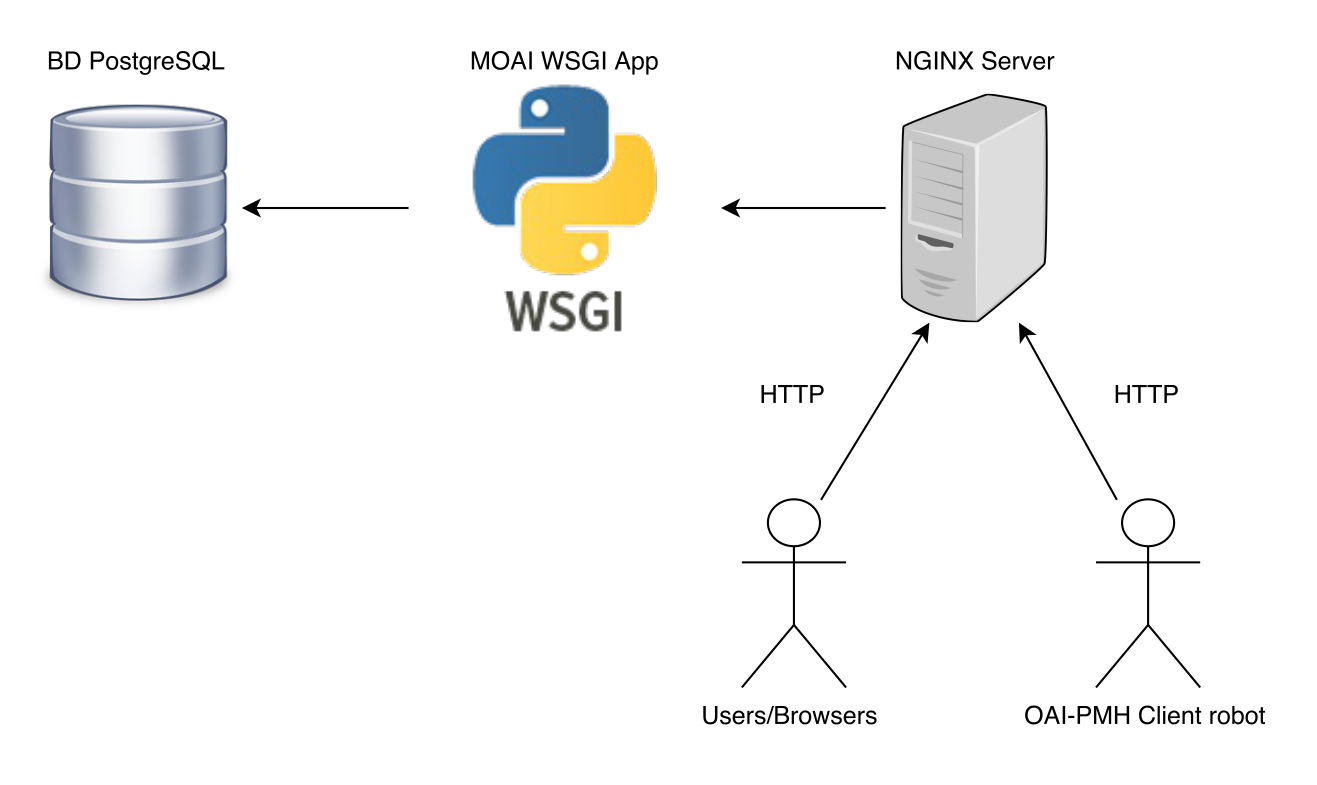
\includegraphics[scale=0.5]{fig/architecture/oai_achitecture}
	\caption{Arquitectura del servidor \acrshort{oaipmh}}
	\label{fig:oai_architecture}
\end{figure}

\section{Diseño del ``mapeo'' de la Base de Datos}

El repositorio de \acrshort{labman} consiste en un conjunto de 120 tablas para almacenar toda la información sobre el grupo de investigación y el propio sistema (véase la figura \ref{fig:labmanmodel}\footnote{Modelo de datos en alta resolución accesible desde \url{https://raw.githubusercontent.com/Alchemy-Meister/PFG/master/fig/dbmodel/high\%20quality/labman\_ud\_models.png}}). Se realizó dicho grafo para tener una visión general de las relaciones de internas del modelo relacional.

Sabiendo que dicho servidor OAI iba a publicar solo la información de las publicaciones de los grupos de investigación, se pudo simplificar el modelo relacional completo y a veces incomprensible, debido a el solapamiento de las lineas que simbolizan relaciones, por uno simplificado y dedicado a las publicaciones (véase la figura \ref{fig:publicationsmodel}\footnote{Modelo de datos en alta resolución accesible desde \url{https://raw.githubusercontent.com/Alchemy-Meister/PFG/master/fig/dbmodel/high\%20quality/publications.png}}), lo cual simplificó la tarea del ``mapeo'', dado que la mayoría de la información podía adquirirse desde dicho grafo a excepción de las relaciones externas a las publicaciones, como pueden ser las entidades \textit{Person}, \textit{Tags} y \textit{Languages}. Para visualizar los atributos de éstas últimas se tuvo que seguir haciendo uso del diagrama completo.

\begin{figure}[!htbp]
	\centering
	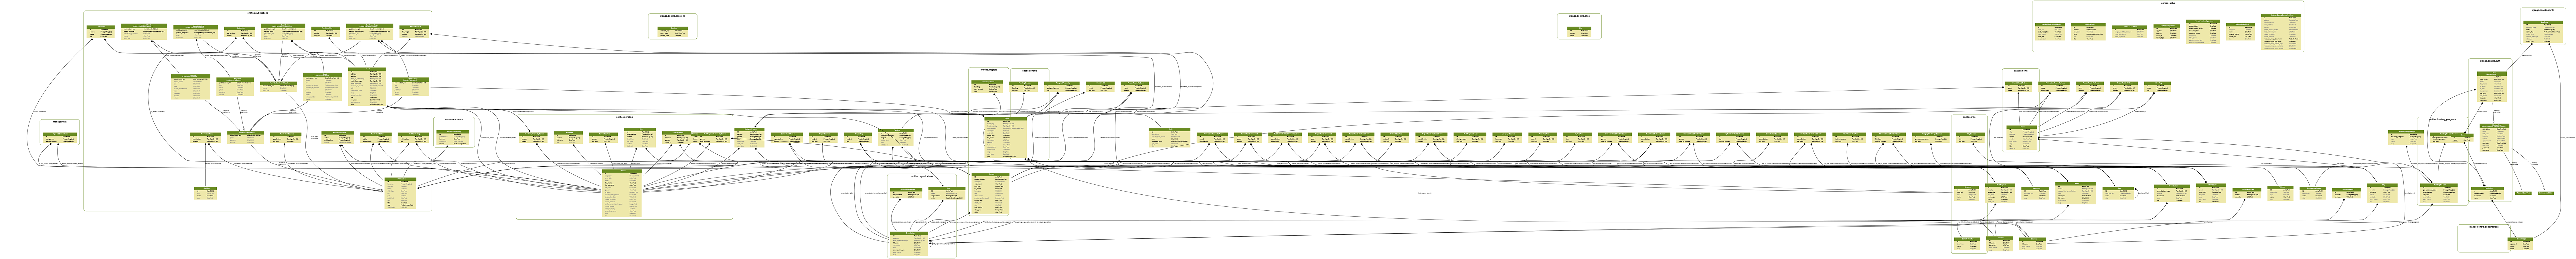
\includegraphics[angle=90, scale=0.072]{fig/dbmodel/labman_model}
	\caption{Modelo de datos relacional completo de \acrshort{labman}}
	\label{fig:labmanmodel}
\end{figure}

Para el desarrollo del servidor se hizo uso de la documentación que proveía la aplicación MOAI para la modificación de la capa de datos. En ésta se detallan los campos de la especificación de \acrshort{dc} que se podían utilizar para el procesado de información y la generación final del \acrshort{xml}. Estos campos y su definición correspondiente son las siguientes:

\begin{itemize}
	\item \textbf{title:} El nombre dado al recursos y por el que es formalmente conocido.
	\item \textbf{creator:} La entidad primaria responsable de la creación del recurso.
	\item \textbf{subject:} El tema que trata el recurso.
	\item \textbf{description:} Documento que puede incluir el resumen o la tabla de contenidos del recurso pero no estar limitado a ellos.
	\item \textbf{publisher:} La entidad responsable de hacer que el recurso este disponible.
	\item \textbf{contributor:} Entidad responsable de hacer contribuciones al recurso.
	\item \textbf{type:} Naturaleza o género del recurso.
	\item \textbf{format:} El formato del fichero o medio físico del documento.
	\item \textbf{identifier:} Una referencia ambigua al recurso.
	\item \textbf{source:} Recursos relacionado que derivan del recurso en cuestión.
	\item \textbf{language:} El lenguaje del recurso.
	\item \textbf{date:} Punto temporal que se asocia con un evento del ciclo de vida del recurso.
	\item \textbf{relation:} Un recurso relacionado.
	\item \textbf{coverage:} La jurisdicción bajo la que un recurso es relevante.
	\item \textbf{rights:} Los derechos propiedad intelectual a los que se ve asociado el recurso.
\end{itemize}

Gracias a esta lista de términos junto con sus definiciones fue necesaria para buscar los campos en la \acrshort{bd} que hacían referencia a estos términos.

Debido al diseño del modelo se descubrió que los tipos de publicaciones, siendo estos actas, ponencias, revistas, artículos de revistas, publicaciones, artículos de publicaciones, libros y secciones de libros, tenían elementos relacionados entre sí. Sin embargo las tesis doctorales estaban formadas por campos completamente independientes por los que se tuvo que realizar un estudio de que elementos de la lista anterior de términos \acrshort{dc} se iban a extraer de la base de datos para las publicaciones y las tesis doctorales por separado quedado el ``mapeo'' resultante tal y como se explica en las subsecciones siguientes.

\subsection{``Mapeo'' de publicaciones}

En esta tabla se pueden visualizar los 

\begin{itemize}
	\item \textbf{title:} entities.publication.publication.title.
	\item \textbf{creator:} person.full\_name relacionado con entities.publication.publicationauthor.author.
	\item \textbf{subject:} tag.name relacionado con entities.publication.publicationtag.
	\item \textbf{description:} entities.publication.publication.abstract.
	\item \textbf{publisher:} entitites.publication.collectionpublication.publisher.
	\item \textbf{type:} entities.publication.publication.childtype.
	\item \textbf{format:} Valor estático ``digital''.
	\item \textbf{identifier:} Concatenación de los campos id y slug de entities.publication.publication
	\item \textbf{language:} language.language\_tag relacionado con entities.publication.publication.language, valor estático ``en'' en caso de null.
	\item \textbf{date:} entities.publication.publication.
\end{itemize}

\begin{figure}[!htbp]
	\centering
	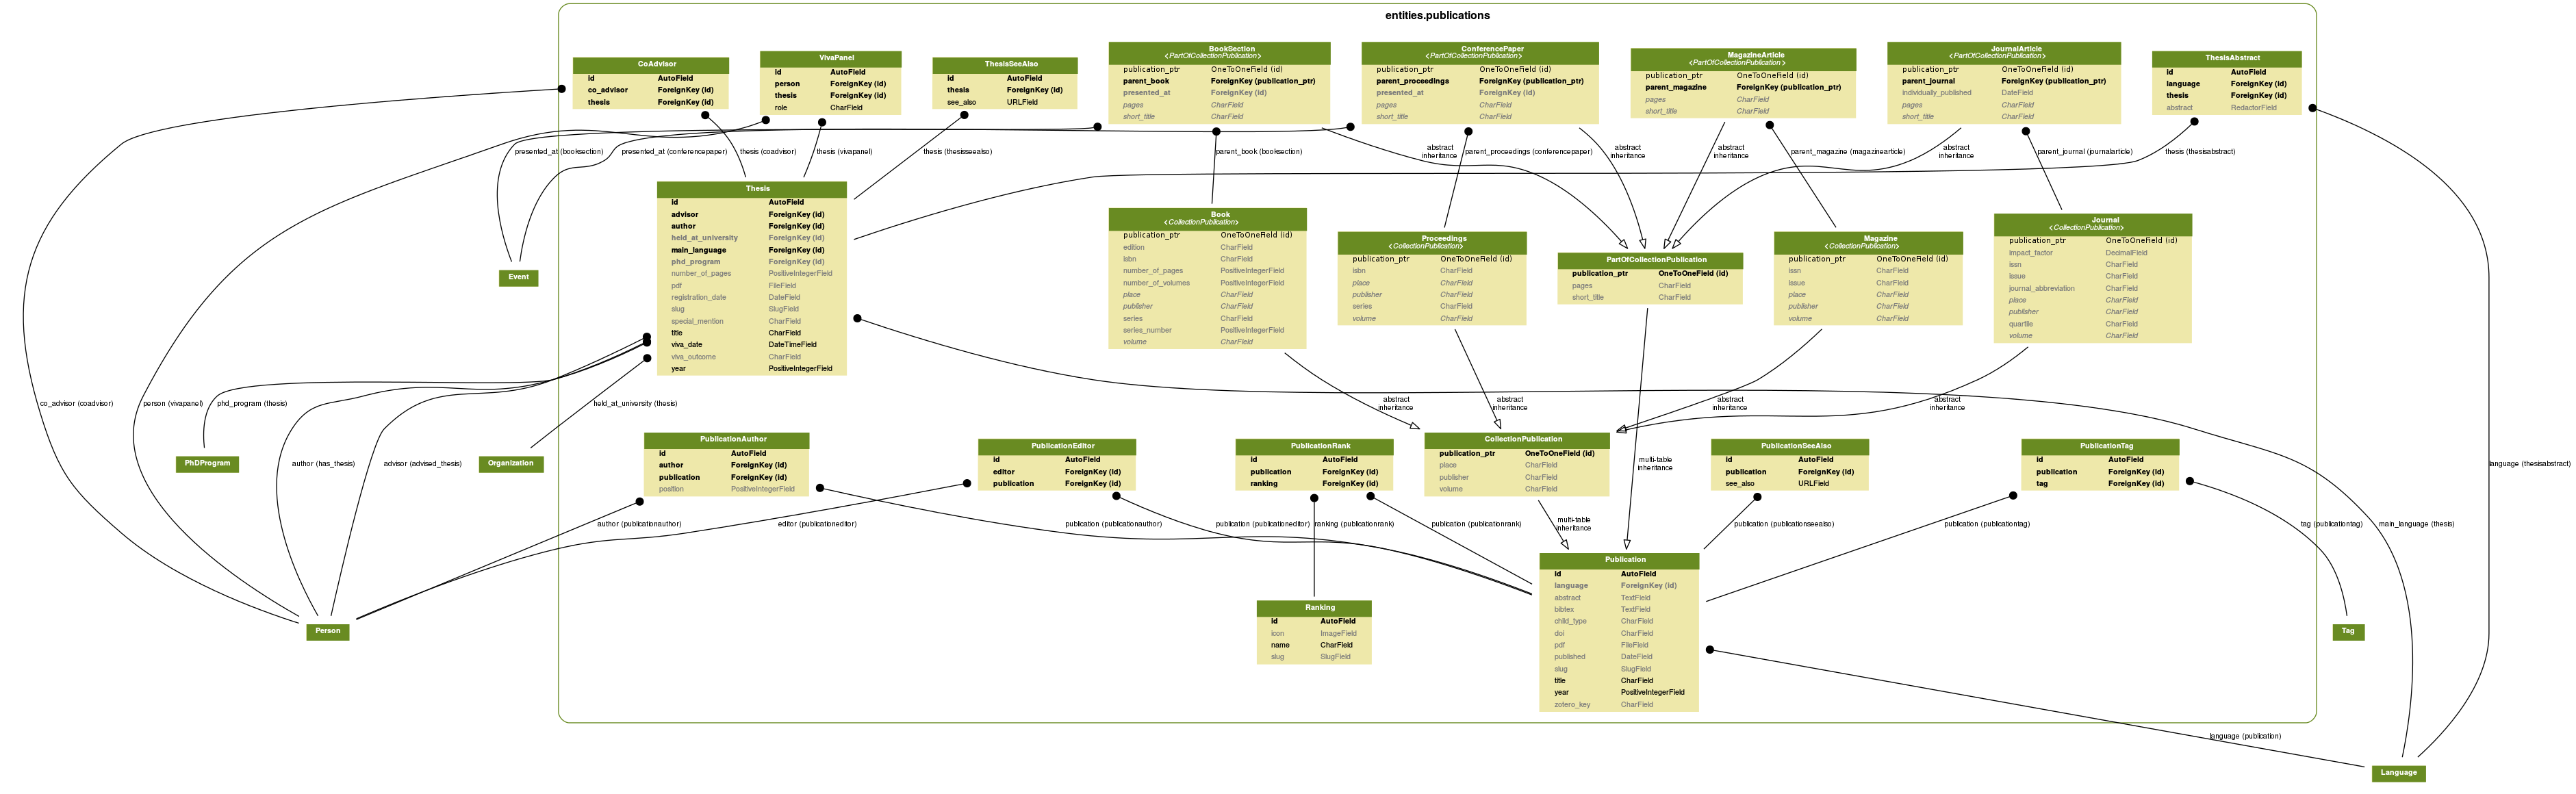
\includegraphics[angle=90, scale=0.17]{fig/dbmodel/publications}
	\caption{Modelo de datos relacional de las publicaciones}
	\label{fig:publicationsmodel}
\end{figure}

\subsection{``Mapeo'' de tesis doctorales}

\begin{itemize}
	\item \textbf{title:} entities.publication.thesis.title.
	\item \textbf{creator:} person.full\_name relacionado con entities.publication.thesis.author.
	\item \textbf{description:} publication.thesisabstract.abstract relacionado con entities.publication.thesis. id.
	\item \textbf{type:} Valor estático ``doctoral dissertation''.
	\item \textbf{format:} Valor estático ``digital''.
	\item \textbf{identifier:} Concatenación de los campos id y slug de entities.publication.publication.
	\item \textbf{language:} language.language\_tag relacionado con entities.publication.thesis.main\_language.
	\item \textbf{date:} entities.publication.thesis.registration\_date, no mostrar en caso de null.
\end{itemize}

\section{Diseño de la aplicación web}

El cliente web es una extensión del sistema ya es uno \acrshort{labman}. La aportación realizada en este proyecto pretende mejorar su funcionalidad mediante la implementación de un buscador avanzado de publicaciones y proyectos para facilitar el acceso la información deseada.

El cliente web ha sido diseñado usando los elementos proporcionados por Django para los elementos estáticos y validación de formularios y a demás se ha utilizado jQuery para añadir funcionalidad dinámica, \acrshort{html} para el contenido y \acrshort{css} y Bootstrap para el diseño.

Al igual que con servidor de MOAI, el diseño de la \acrshort{bd} ya venía preestablecido, pero se ha requerido hacer un estudio de las entidades del modelo de datos relacionados con las publicaciones, como ya ha podido verse en la figura \ref{fig:publicationsmodel}, así como el modelo de proyectos (véase la figura \ref{fig:projectsmodel}\footnote{Modelo de datos en alta resolución accesible desde \url{https://raw.githubusercontent.com/Alchemy-Meister/PFG/master/fig/dbmodel/high\%20quality/projects.png}}), para realizar el filtrado de la información a partir de un subconjunto de sus facetas.

Django se basa en la arquitectura \acrshort{mvc} (véase la figura \ref{fig:mvc}) en la que el usuario interactua con el controlador actualizando la vista para introducir los valores en las facetas sobre las que desea filtrar la información y al realizar comenzar la búsqueda, el controlador consulta el modelo, obtiene la información requerida por el usuario y actualiza la vista.

\begin{figure}[!htbp]
	\centering
	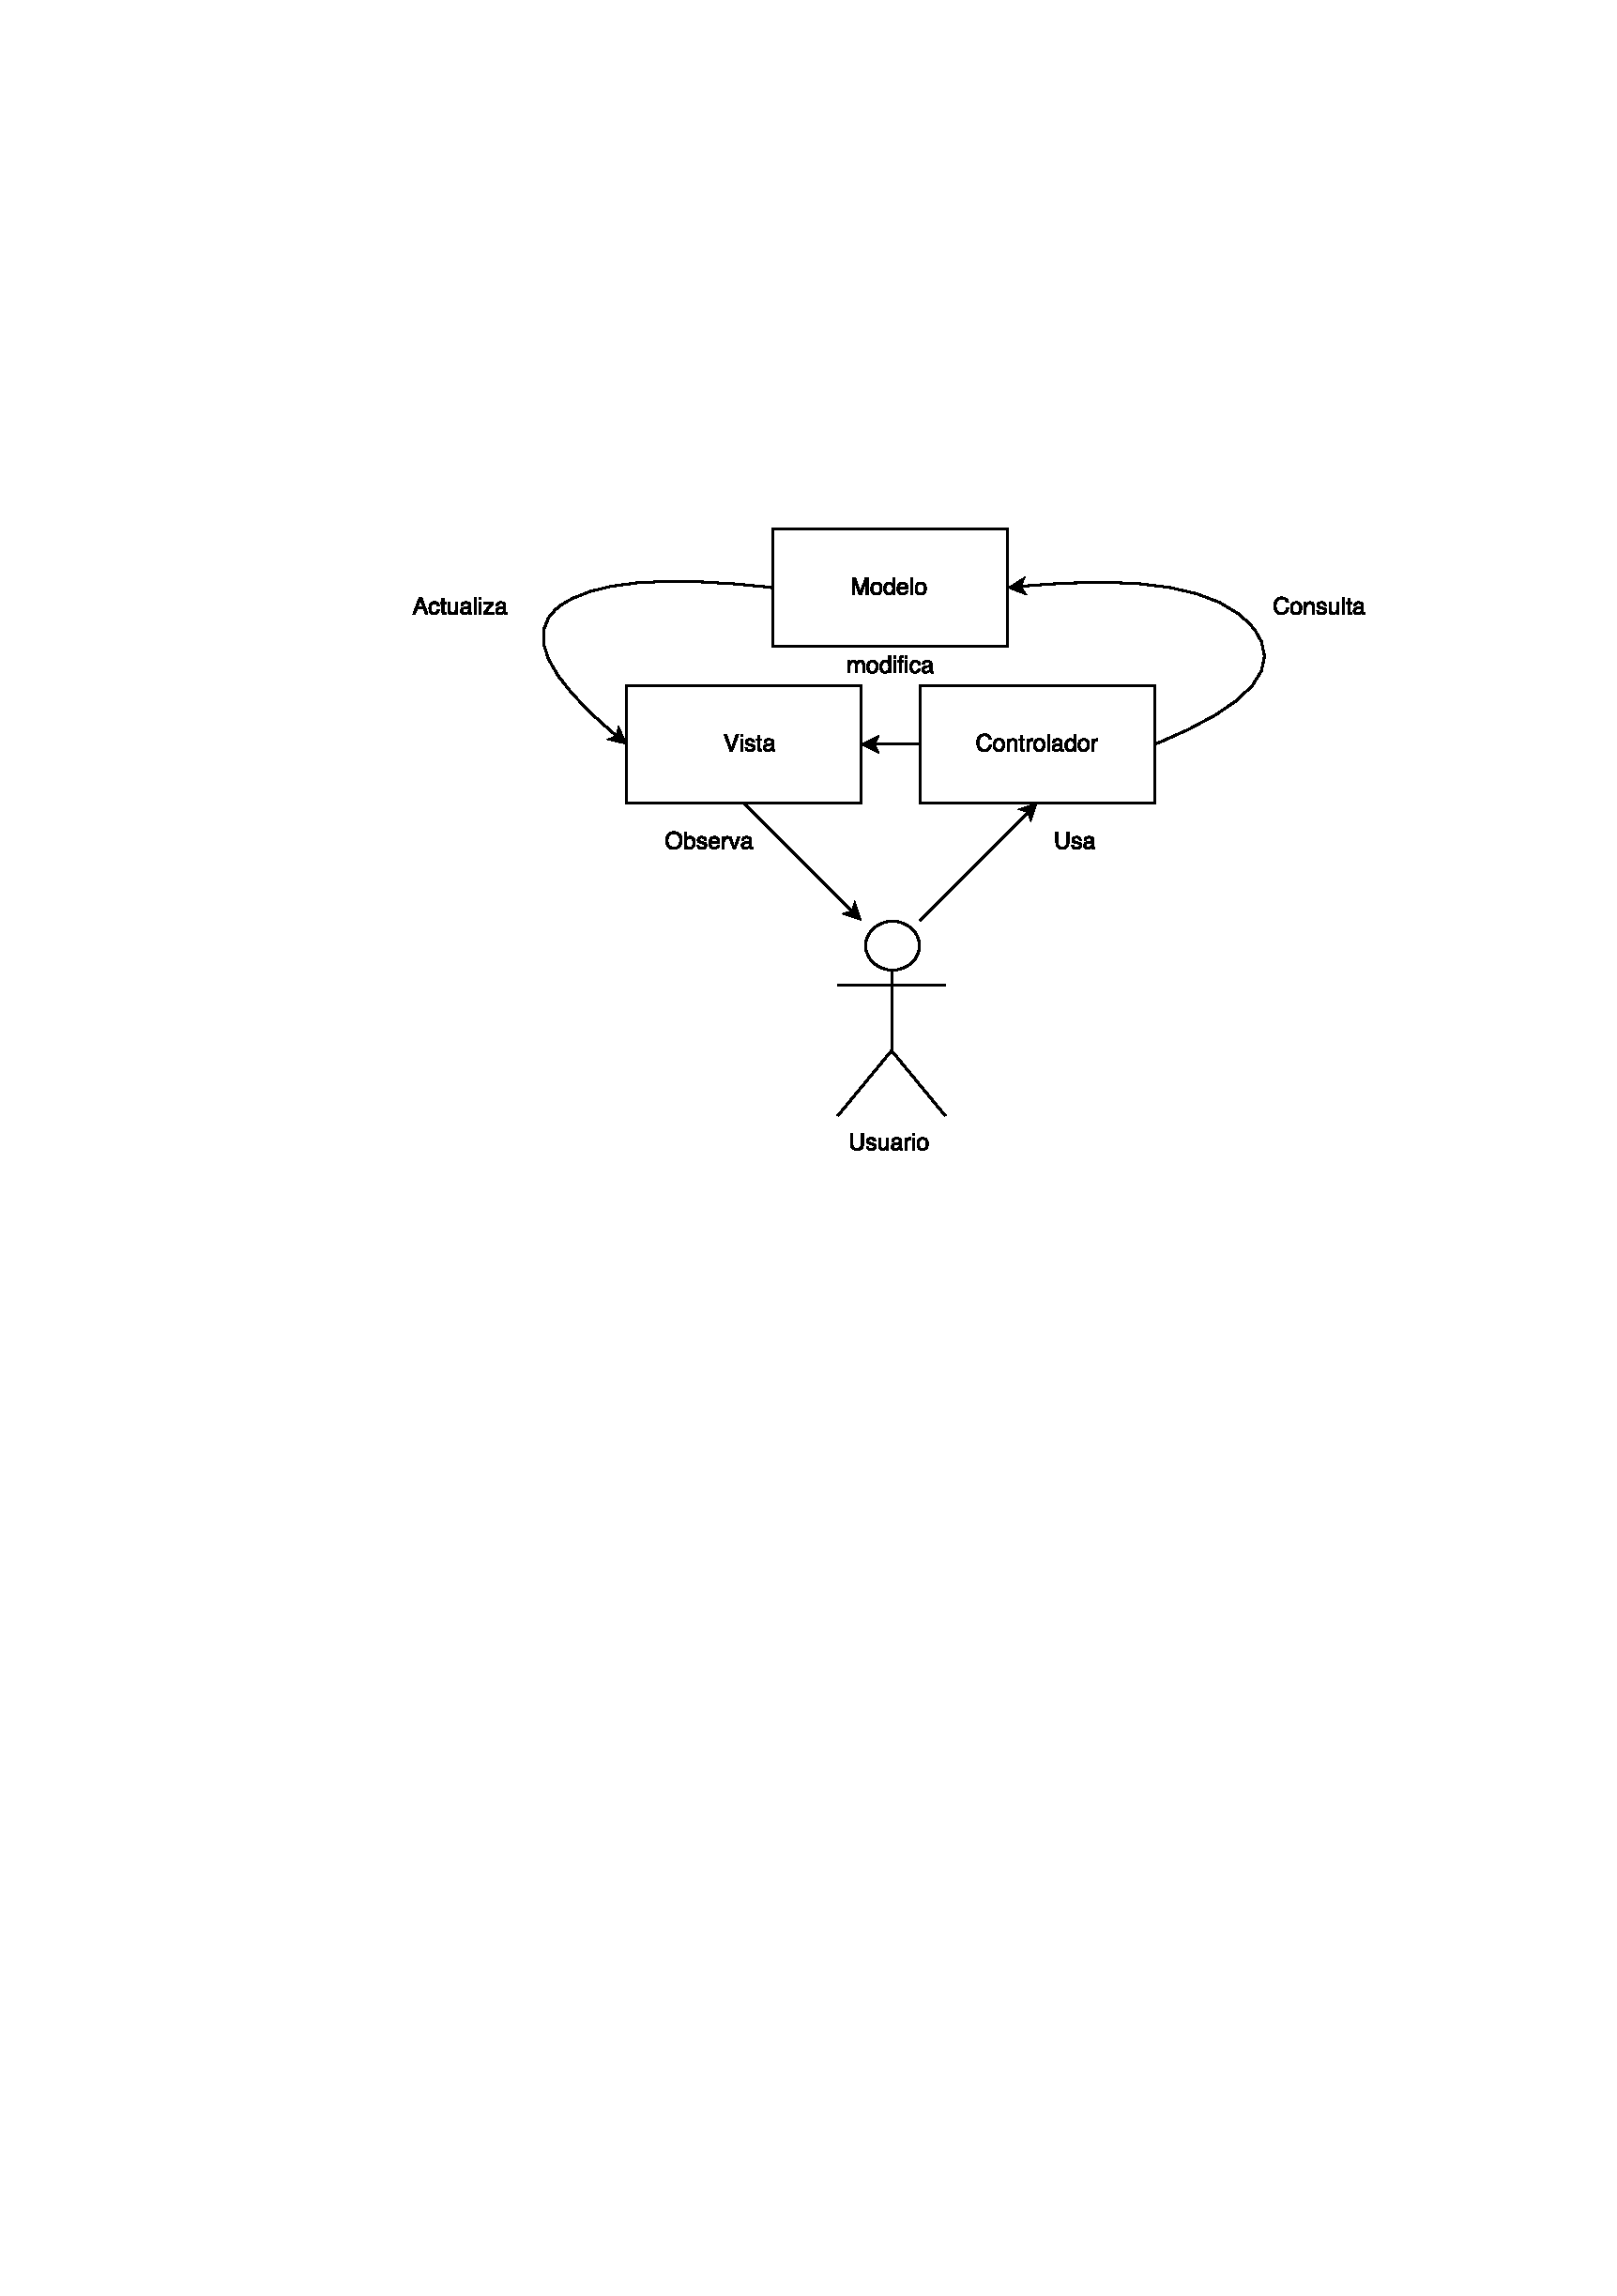
\includegraphics[scale=0.6]{fig/mvc}
	\caption{Arquitectura \acrshort{mvc} del cliente web}
	\label{fig:mvc}
\end{figure}

\begin{figure}[!htbp]
	\centering
	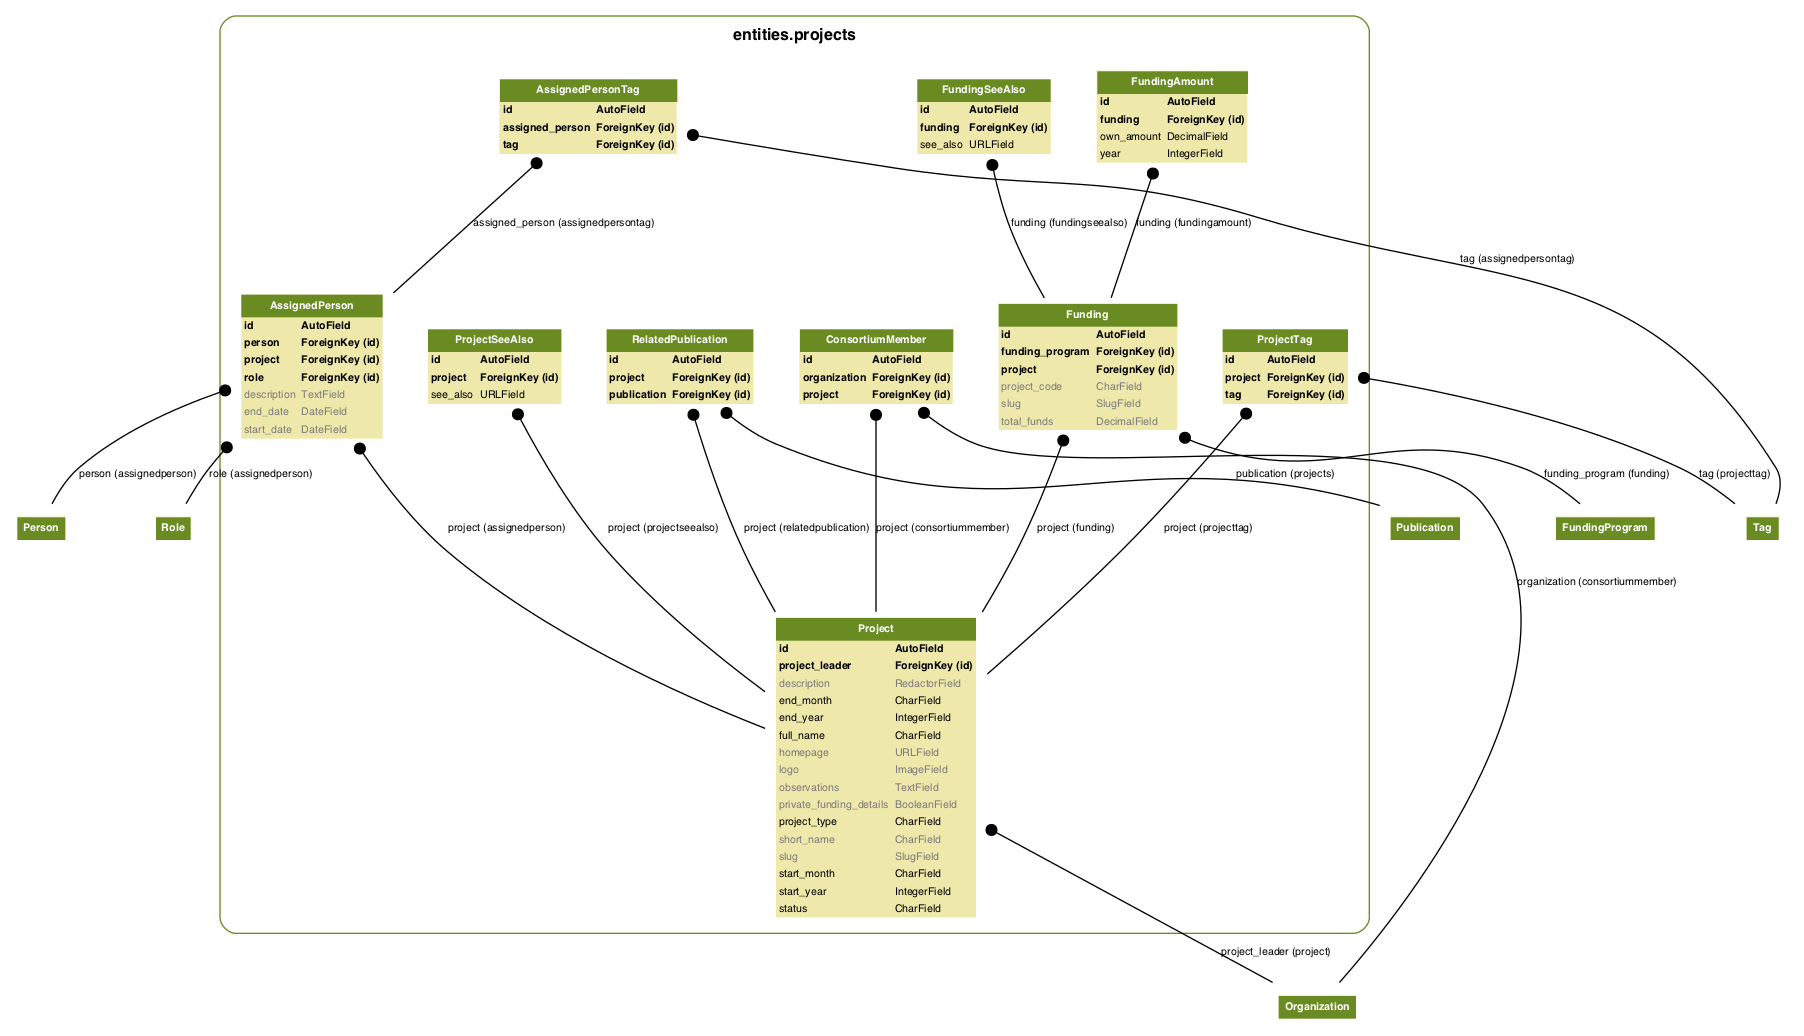
\includegraphics[angle=90, scale=0.35]{fig/dbmodel/projects}
	\caption{Modelo de datos relacional de las proyectos}
	\label{fig:projectsmodel}
\end{figure}


\chapter{Consideracones sobre la implementación}
\chapter{Plan de pruebas}

\section{Visión general}

Durante el desarrollo del proyecto se han realizado diversas pruebas para asegurar la fiabilidad del sistema en completo, tratando de minimizar el número de fallos que pueden ocurrir. En este capítulo se van a explicar algunas de las pruebas realizadas.

\section{Pruebas del servidor OAI-PMH}

Además de haber realizado las rutinarias pruebas unitarias, para comprobar que el servidor genera respuestas \acrshort{xml} válidas ajustandose a la especificación del protocolo \acrshort{oaipmh}, se ha optado por utilizar una herramienta web que facilita esta verificación, el \acrshort{oaipmh} validator.

Se han realizados las siguientes pruebas mediante el uso de esta herramienta que verifican que el servidor funciona correctamente y por tanto los clientes que realicen las peticiones reciben las respuestas apropiadas:

\subsection{Verificación del comando Idenfity}

En está comprobación se ha copiado la respuesta generada por el servidor \acrshort{oaipmh} a la petición \textit{Identify}. Como se puede ver en la figura \ref{fig:identify}, el validador ha comprobado que el documento \acrshort{xml} es válido, que cumple con el esquema de la versión 2.0 del protocolo y que la dirección del correo electrónico dispuesto para facilitar el soporte a incidencias es correcto.

\begin{figure}[!htbp]
	\centering
	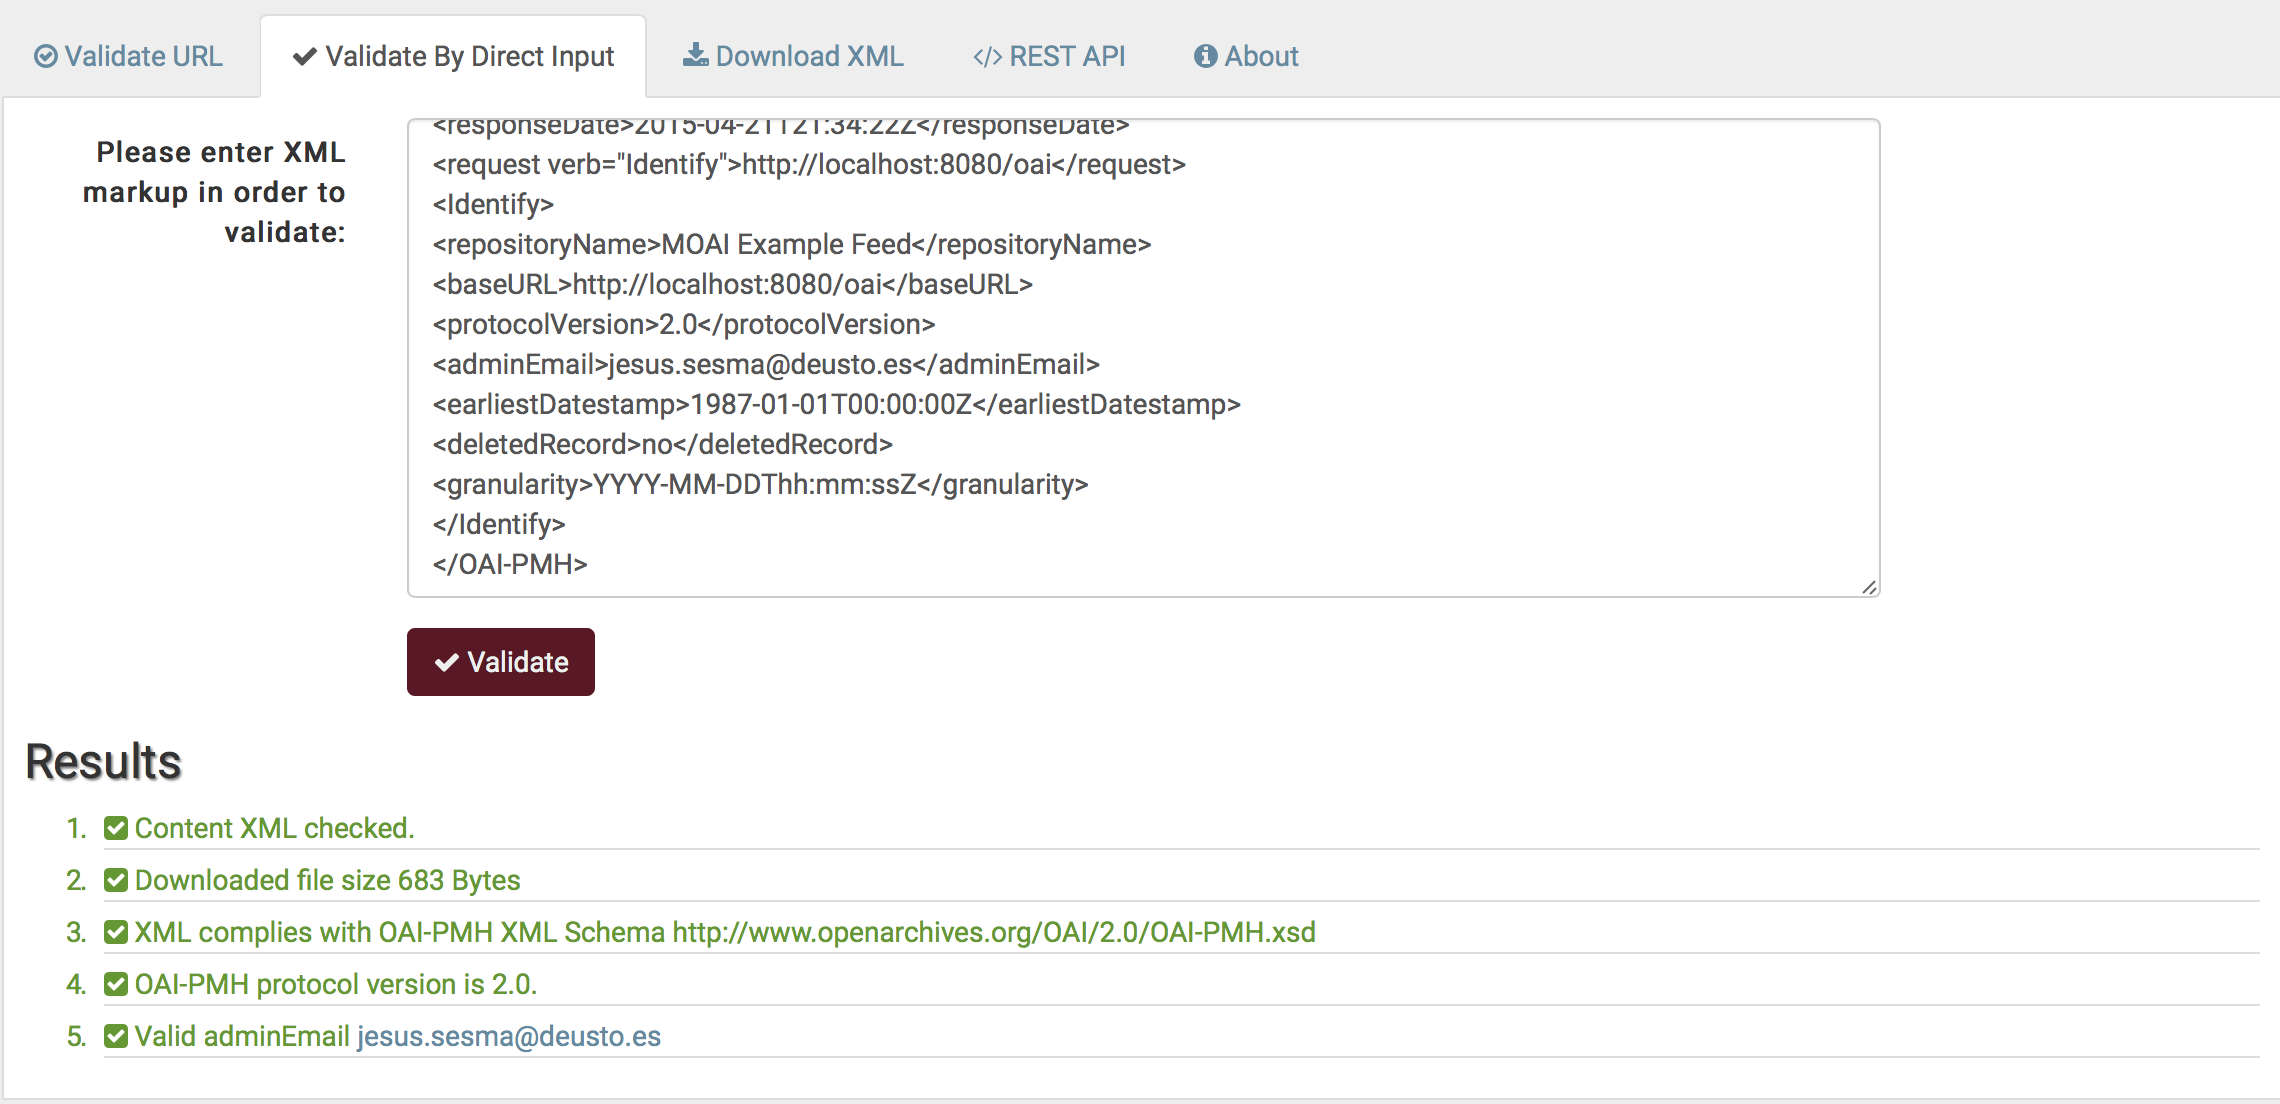
\includegraphics[scale=0.32]{fig/oaipmh_validations/Identify}
	\caption{Validación satisfactoria del comando Identify}
	\label{fig:identify}
\end{figure}

\subsection{Verificación del comando ListMetadataFormats}

En está comprobación se ha copiado la respuesta generada por el servidor \acrshort{oaipmh} a la petición \textit{ListMetadataFormats}. Como se puede ver en la figura \ref{fig:listmetadataformats}, el validador ha comprobado que el documento \acrshort{xml} es válido, que cumple con el esquema de la versión 2.0 del protocolo. Por último lista los esquemas que soporta el servidor \acrshort{oaipmh}, siendo el primero de estos \acrlong{dc}, el formato bibliográfico estándar de soporte obligatorio, y el segundo un esquema opcional \acrfull{mods}\cite{MODS}.

\begin{figure}[!htbp]
	\centering
	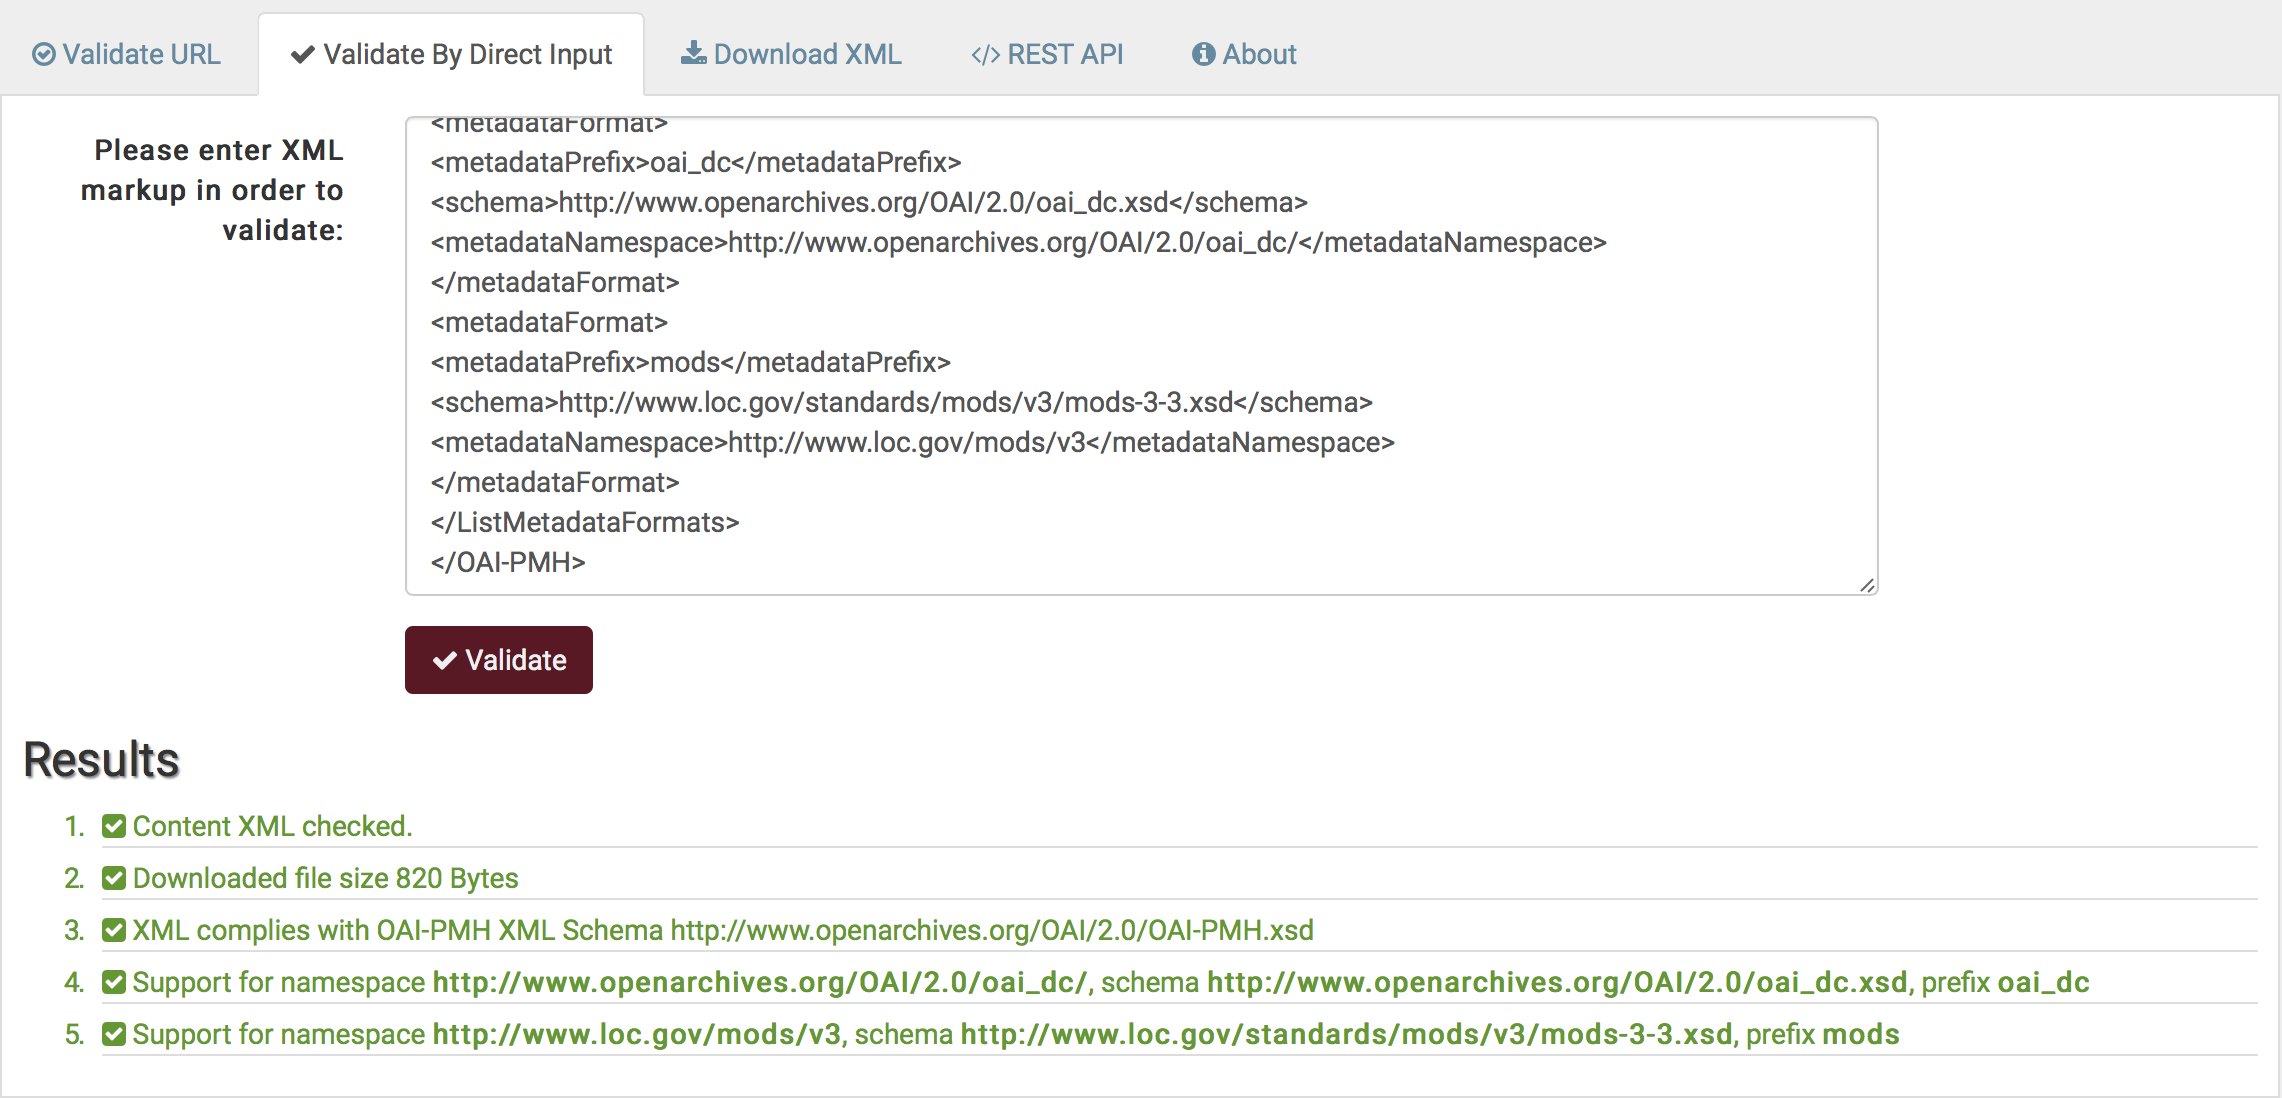
\includegraphics[scale=0.32]{fig/oaipmh_validations/ListMetadataFormats}
	\caption{Validación satisfactoria del comando ListMetadataFormats}
	\label{fig:listmetadataformats}
\end{figure}

\subsection{Verificación del comando ListSets}

\begin{figure}[!htbp]
	\centering
	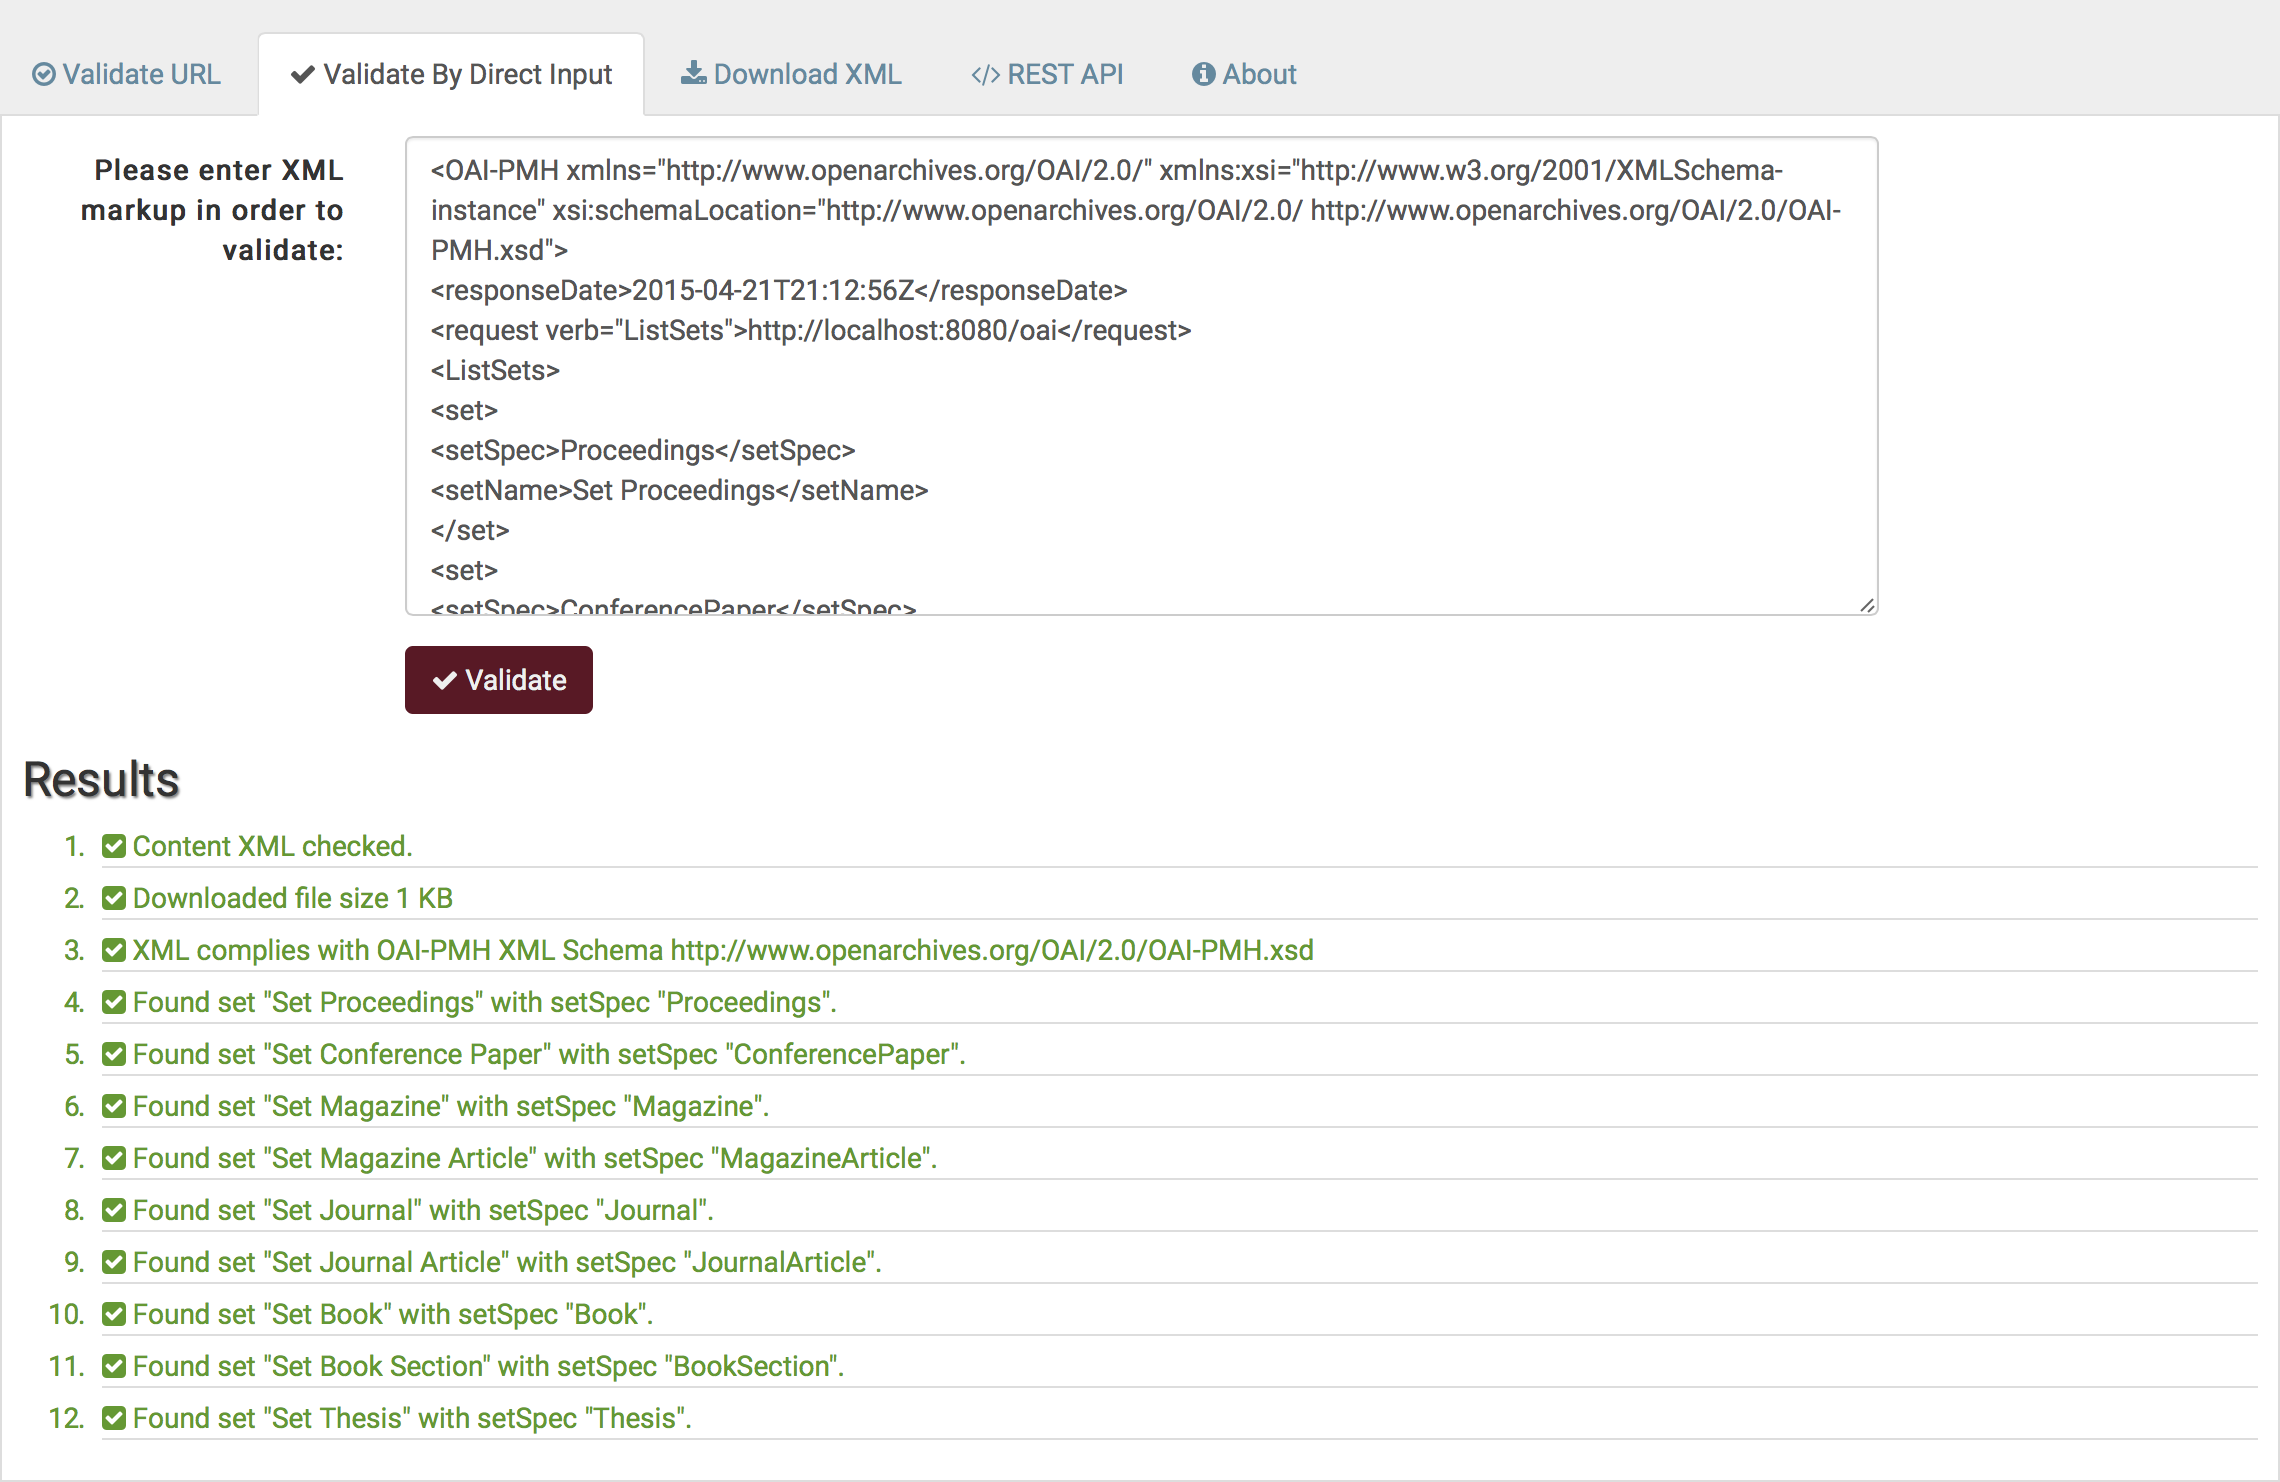
\includegraphics[scale=0.32]{fig/oaipmh_validations/ListSets}
	\caption{Validación satisfactoria del comando ListSets}
	\label{fig:listsets}
\end{figure}

\subsection{Verificación del comando ListIdentifiers}

\begin{figure}[!htbp]
	\centering
	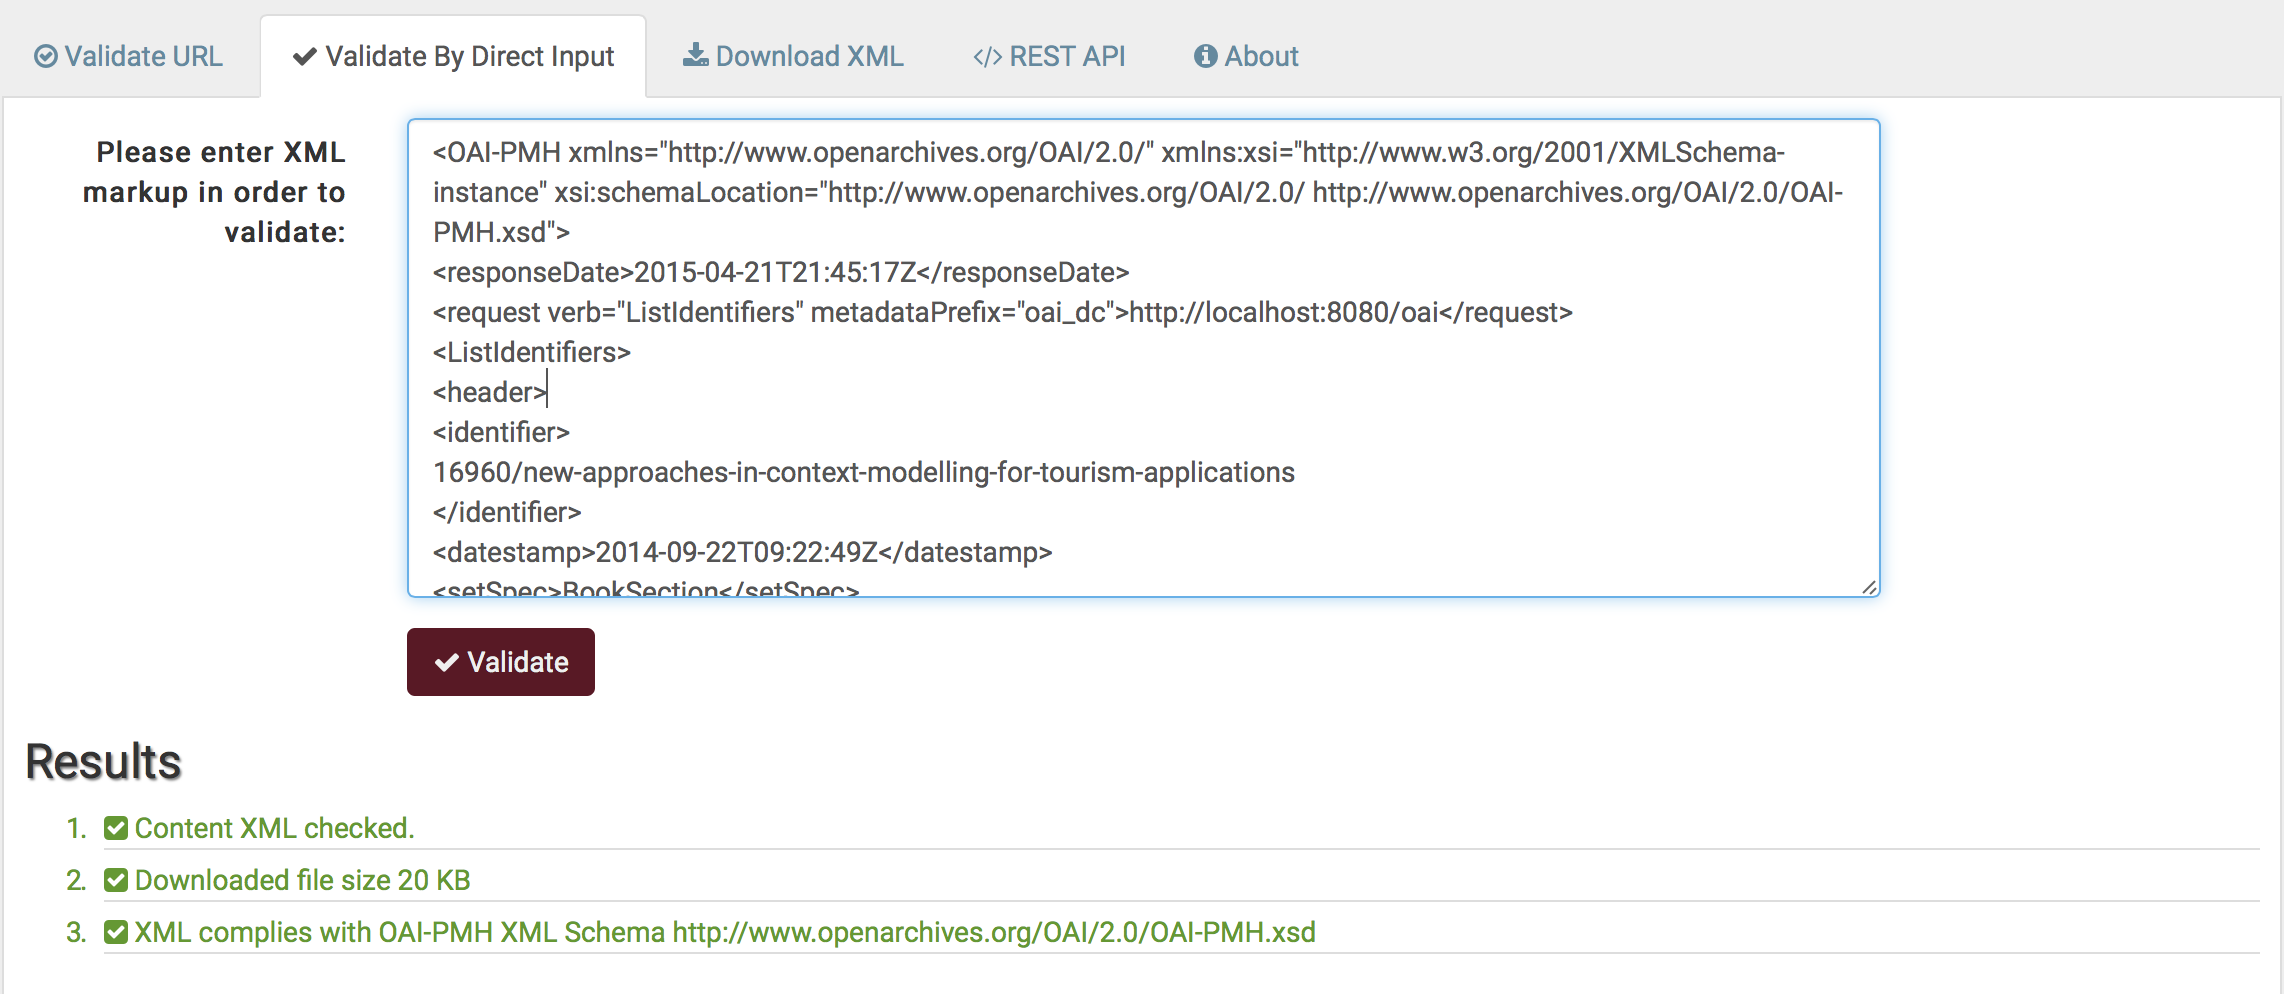
\includegraphics[scale=0.32]{fig/oaipmh_validations/ListIdentifiers}
	\caption{Validación satisfactoria del comando ListIdentifiers}
	\label{fig:listidentifiers}
\end{figure}

\chapter{Manual de usuario}

\section{Visión general}

En este capítulo se muestran los manuales que explican paso a paso cómo hacer uso de las herramientas desarrolladas a nivel de usuario. Los mismos se dividen en dos manuales:

\begin{itemize}
	\item \textbf{Manual de usuario del servidor \acrshort{oaipmh}:} este manual abarca todas las posibles consultas que se pueden realizar al servidor mediante un cliente \acrshort{oaipmh} como puede ser el propio \acrshort{oaipmh} validator o los clientes que dispone la comunidad \acrshort{oai}.
	\item \textbf{Manual de usuario de la aplicación web:} este manual abarca todos los pasos para realizar las búsquedas avanzadas en proyectos y publicaciones desde el portal web \acrshort{labman}.
\end{itemize}

\section{Manual de usuario del servidor OAI-PMH}

Este manual pretende dar a conocer los comandos a los que responde el servidor \acrshort{oaipmh}, para que por medio de clientes \acrshort{oai} se pueda extraer la información del repositorio puesto en producción en la \acrshort{url} \url{http://apps.morelab.deusto.es/labman/oai}. Este manual pone como ejemplo como descargar el contenido \acrshort{xml} a través del mismo navegador o de la herramienta \acrshort{oaipmh} validator (\url{http://validator.oaipmh.com/}). Si se usan herramientas más sofisticadas como las facilitadas por la comunidad, se podrán procesar estos \acrshort{xml} y almacenarlos en una \acrshort{bd} de forma automatizada, para más información sobre estas herramientas consultad el siguiente enlace: \url{https://www.openarchives.org/pmh/tools/tools.php}.

El servidor admite tanto las siguientes peticiones \acrshort{http} GET como POST por parte de los clientes, explicados en la sección \ref{sec:oaipmh}:

\begin{itemize}
	\item Identify
	\item ListMetadataFormats
	\item ListSets
	\item ListIdentifiers
	\item ListRecords
	\item GetRecord
\end{itemize}

\subsection{Obtener la información del comando Identify}

Para descargar la información del comando Identify desde el propio navegador ha de realizarse una petición GET a la \acrshort{url} del servidor especificando dicho verbo mediante un \textit{query string}.

Para descargarla desde \acrshort{oaipmh} validator es necesario introducir la \acrshort{url} del repositorio \acrshort{oai} y pulsar en el botón validate, si se introduce una \acrshort{url} de un repositorio válida aparecerán las operaciones disponibles del servidor.

Se deberá seleccionar el comando \textit{Identify} y escoger la pestaña \textit{\acrshort{xml} result} para acceder a la información tal y como se muestra en la figura \ref{fig:download_identify}.

\begin{figure}[!htbp]
	\centering
	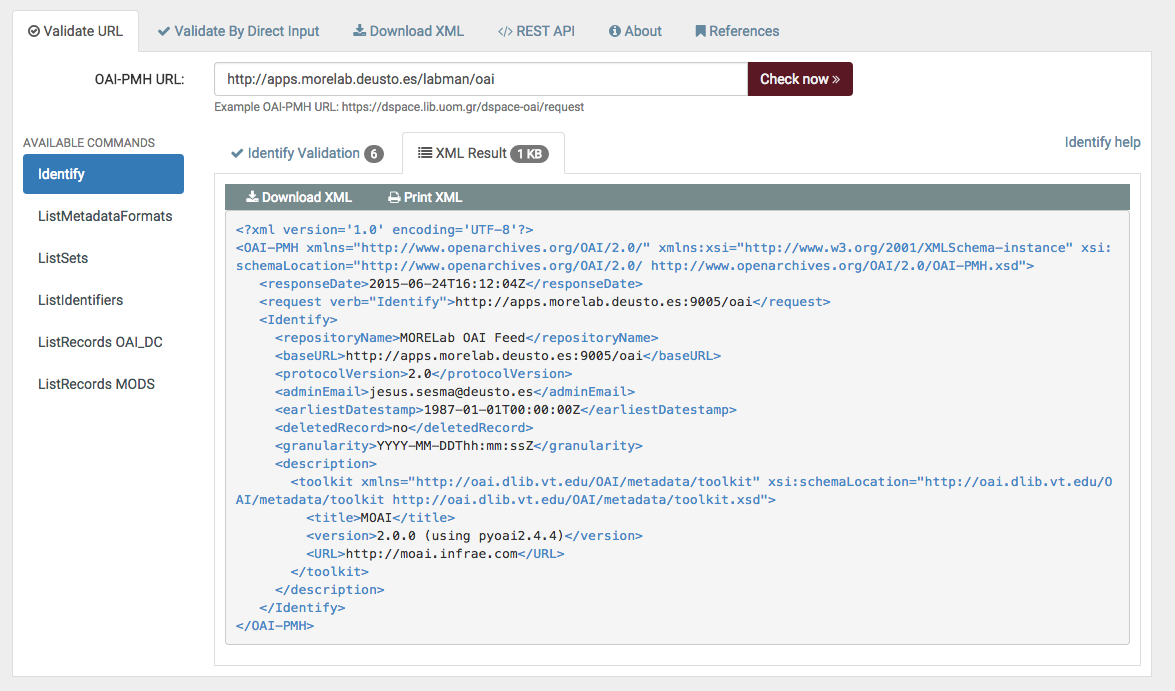
\includegraphics[scale=0.31]{fig/download_oai/download_identify}
	\caption{Información del comando Identify desde \acrshort{oaipmh} validator}
	\label{fig:download_identify}
\end{figure}

\subsection{Obtener la información del comando ListMetadataFormats}

Para descargar la información del comando ListMetadataFormats desde el propio navegador ha de realizarse una petición GET a la \acrshort{url} del servidor especificando dicho verbo mediante un \textit{query string}.

Al igual que para el comando \textit{Identify}, para descargarla desde \acrshort{oaipmh} validator es necesario introducir la \acrshort{url} del repositorio \acrshort{oai} y pulsar en el botón validate, si se introduce una \acrshort{url} de un repositorio válida aparecerán las operaciones disponibles del servidor.

Se deberá seleccionar el comando \textit{ListMetadataFormats} y escoger la pestaña \textit{\acrshort{xml} result} para acceder a la información.

\subsection{Obtener la información del comando ListSets}

Para descargar la información del comando ListSets desde el propio navegador ha de realizarse una petición GET a la \acrshort{url} del servidor especificando dicho verbo mediante un \textit{query string}.

Al igual que para el comando \textit{Identify}, para descargarla desde \acrshort{oaipmh} validator es necesario introducir la \acrshort{url} del repositorio \acrshort{oai} y pulsar en el botón validate, si se introduce una \acrshort{url} de un repositorio válida aparecerán las operaciones disponibles del servidor.

Se deberá seleccionar el comando \textit{ListSets} y escoger la pestaña \textit{\acrshort{xml} result} para acceder a la información.

\subsection{Obtener la información del comando ListIdentifiers}

Para descargar la información del comando ListSets desde el propio navegador ha de realizarse una petición GET a la \acrshort{url} del servidor especificando dicho verbo y el formato bibliográfico en el que se desea que se devuelva la consulta mediante \textit{query strings}, pudiendo filtrar por \textit{set}, \textit{from} y \textit{to}.

Esta consulta devolverá los cien primeros identificadores del repositorio, además de una clave para continuar la consulta de los siguientes cien elementos, cada vez que se quiera continuar la consulta se deberá hacer uso de dicho código, hasta que la consulta resultante disponga menos de cien recursos. 

Al igual que para el comando \textit{Identify}, para descargarla desde \acrshort{oaipmh} validator es necesario introducir la \acrshort{url} del repositorio \acrshort{oai} y pulsar en el botón validate, si se introduce una \acrshort{url} de un repositorio válida aparecerán las operaciones disponibles del servidor.

Se deberá seleccionar el comando \textit{ListSets} y escoger la pestaña \textit{\acrshort{xml} result} para acceder a la información, sin embargo la información de este comando estará limitado a los cien primero recursos del repositorio.

\subsection{Obtener la información del comando ListRecords}

Para descargar la información del comando ListRecords desde el propio navegador ha de realizarse una petición GET a la \acrshort{url} del servidor especificando dicho verbo y el formato bibliográfico en el que se desea que se devuelva la consulta mediante \textit{query strings}, puediendo filtrar por \textit{set}, \textit{from} y \textit{to}.

Esta consulta devolverá los cien primeros identificadores del repositorio, además de una clave para continuar la consulta de los siguientes cien elementos, cada vez que se quiera continuar la consulta se deberá hacer uso de dicho código, hasta que la consulta resultante disponga menos de cien recursos.

\begin{figure}[!htbp]
	\centering
	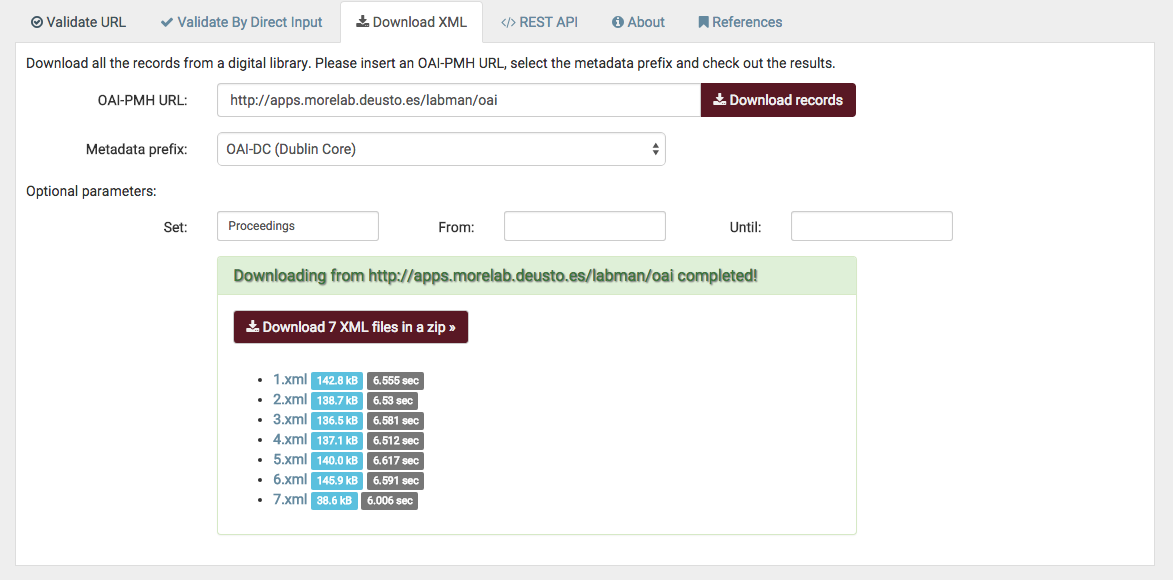
\includegraphics[scale=0.31]{fig/download_oai/download_listrecords}
	\caption{Información del comando ListRecords desde \acrshort{oaipmh} validator}
	\label{fig:download_listrecords}
\end{figure}

Para descargar la información del comando ListRecords se deberá acceder a la pestaña \textit{Download} \acrshort{xml} e introducir la \acrshort{url} del repositorio. Adicionalmente se puede filtrar los recursos por \textit{set} y por rango temporal \textit{from} y \textit{to}.

Por último se deberá pulsar en el botón \textit{Download records} para que genere los documentos \acrshort{xml}, estos se podrán descargar tanto individualmente como empaquetados en un zip tal y como se puede ver en la imagen \ref{fig:download_listrecords}.

\subsection{Obtener la información del comando GetRecord}

Para descargar la información del comando GetRecord desde el propio navegador ha de realizarse una petición GET a la \acrshort{url} del servidor especificando dicho verbo y el formato bibliográfico en el que se desea que se devuelva la consulta mediante \textit{query strings}

Para descargar la información de un recurso en concreto al igual que para \textit{ListRecords} hay que acceder a la pestaña \textit{Download} \acrshort{xml} e introducir la url del repositorio junto los \textit{query string} en la propia \acrshort{url} del repositorio para descargar la información como se muestra en la figura \ref{fig:download_getrecord}.

\begin{figure}[!htbp]
	\centering
	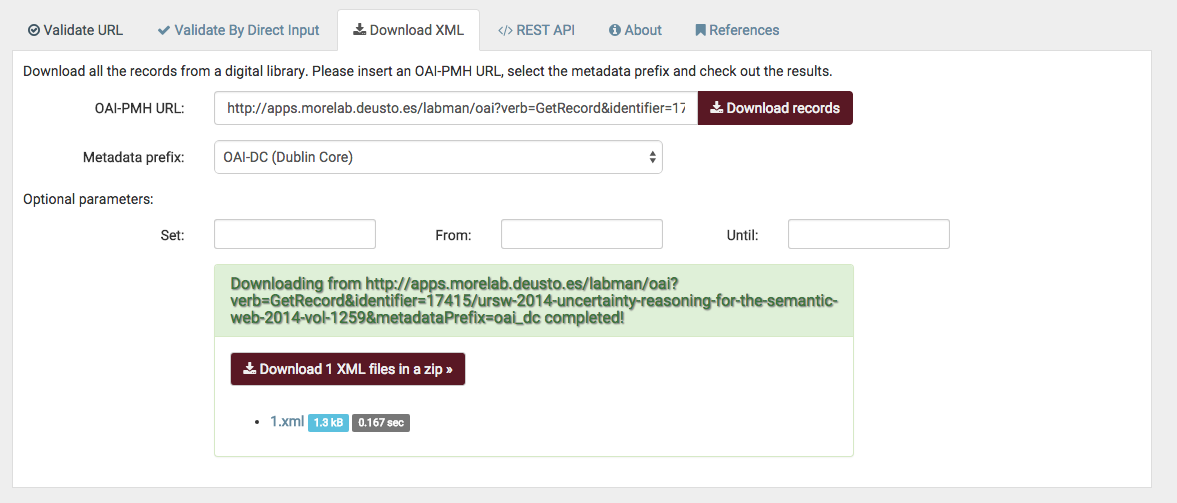
\includegraphics[scale=0.31]{fig/download_oai/download_getrecord}
	\caption{Información del comando GetRecord desde \acrshort{oaipmh} validator}
	\label{fig:download_getrecord}
\end{figure}

\section{Manual de usuario de la aplicación web}

\subsection{Página principal de LabMan}

Nada más acceder al portal web de \acrshort{labman}, se visualiza su \textit{homepage} (ver figura \ref{fig:morelab_homepage}). En ella se muestra una imagen con los miembros del grupo, la descripción y las últimas noticias relacionadas con el equipo de investigación en cuestión.

Por otra parte, se presenta una barra de navegación, con todas las siguientes opciones que ofrece \acrshort{labman} por defecto:

\begin{itemize}
	\item \textbf{News:} Muestra un buscador paginado con el registro \acrfull{rss} de las noticias relacionadas con el equipo de investigación.
	\item \textbf{Projects:} Muestra un buscador paginado con el registro de los proyectos que involucran a los miembros del equipo de investigación.
	\item \textbf{Publications:} Muestra un buscador paginado con el registro de las publicaciones redactadas por los miembros del equipo de investigación.
	\item \textbf{Member:} Muestra la lista con los integrantes del grupo de investigación.
	\item \textbf{Charts:} Muestra el menú por el que se accederán a las gráficas formadas a partir de los datos de los apartados anteriores.
	\item \textbf{About:} Muestra información adicional relacionada con el grupo de investigación.
\end{itemize}

\begin{figure}[!htbp]
	\centering
	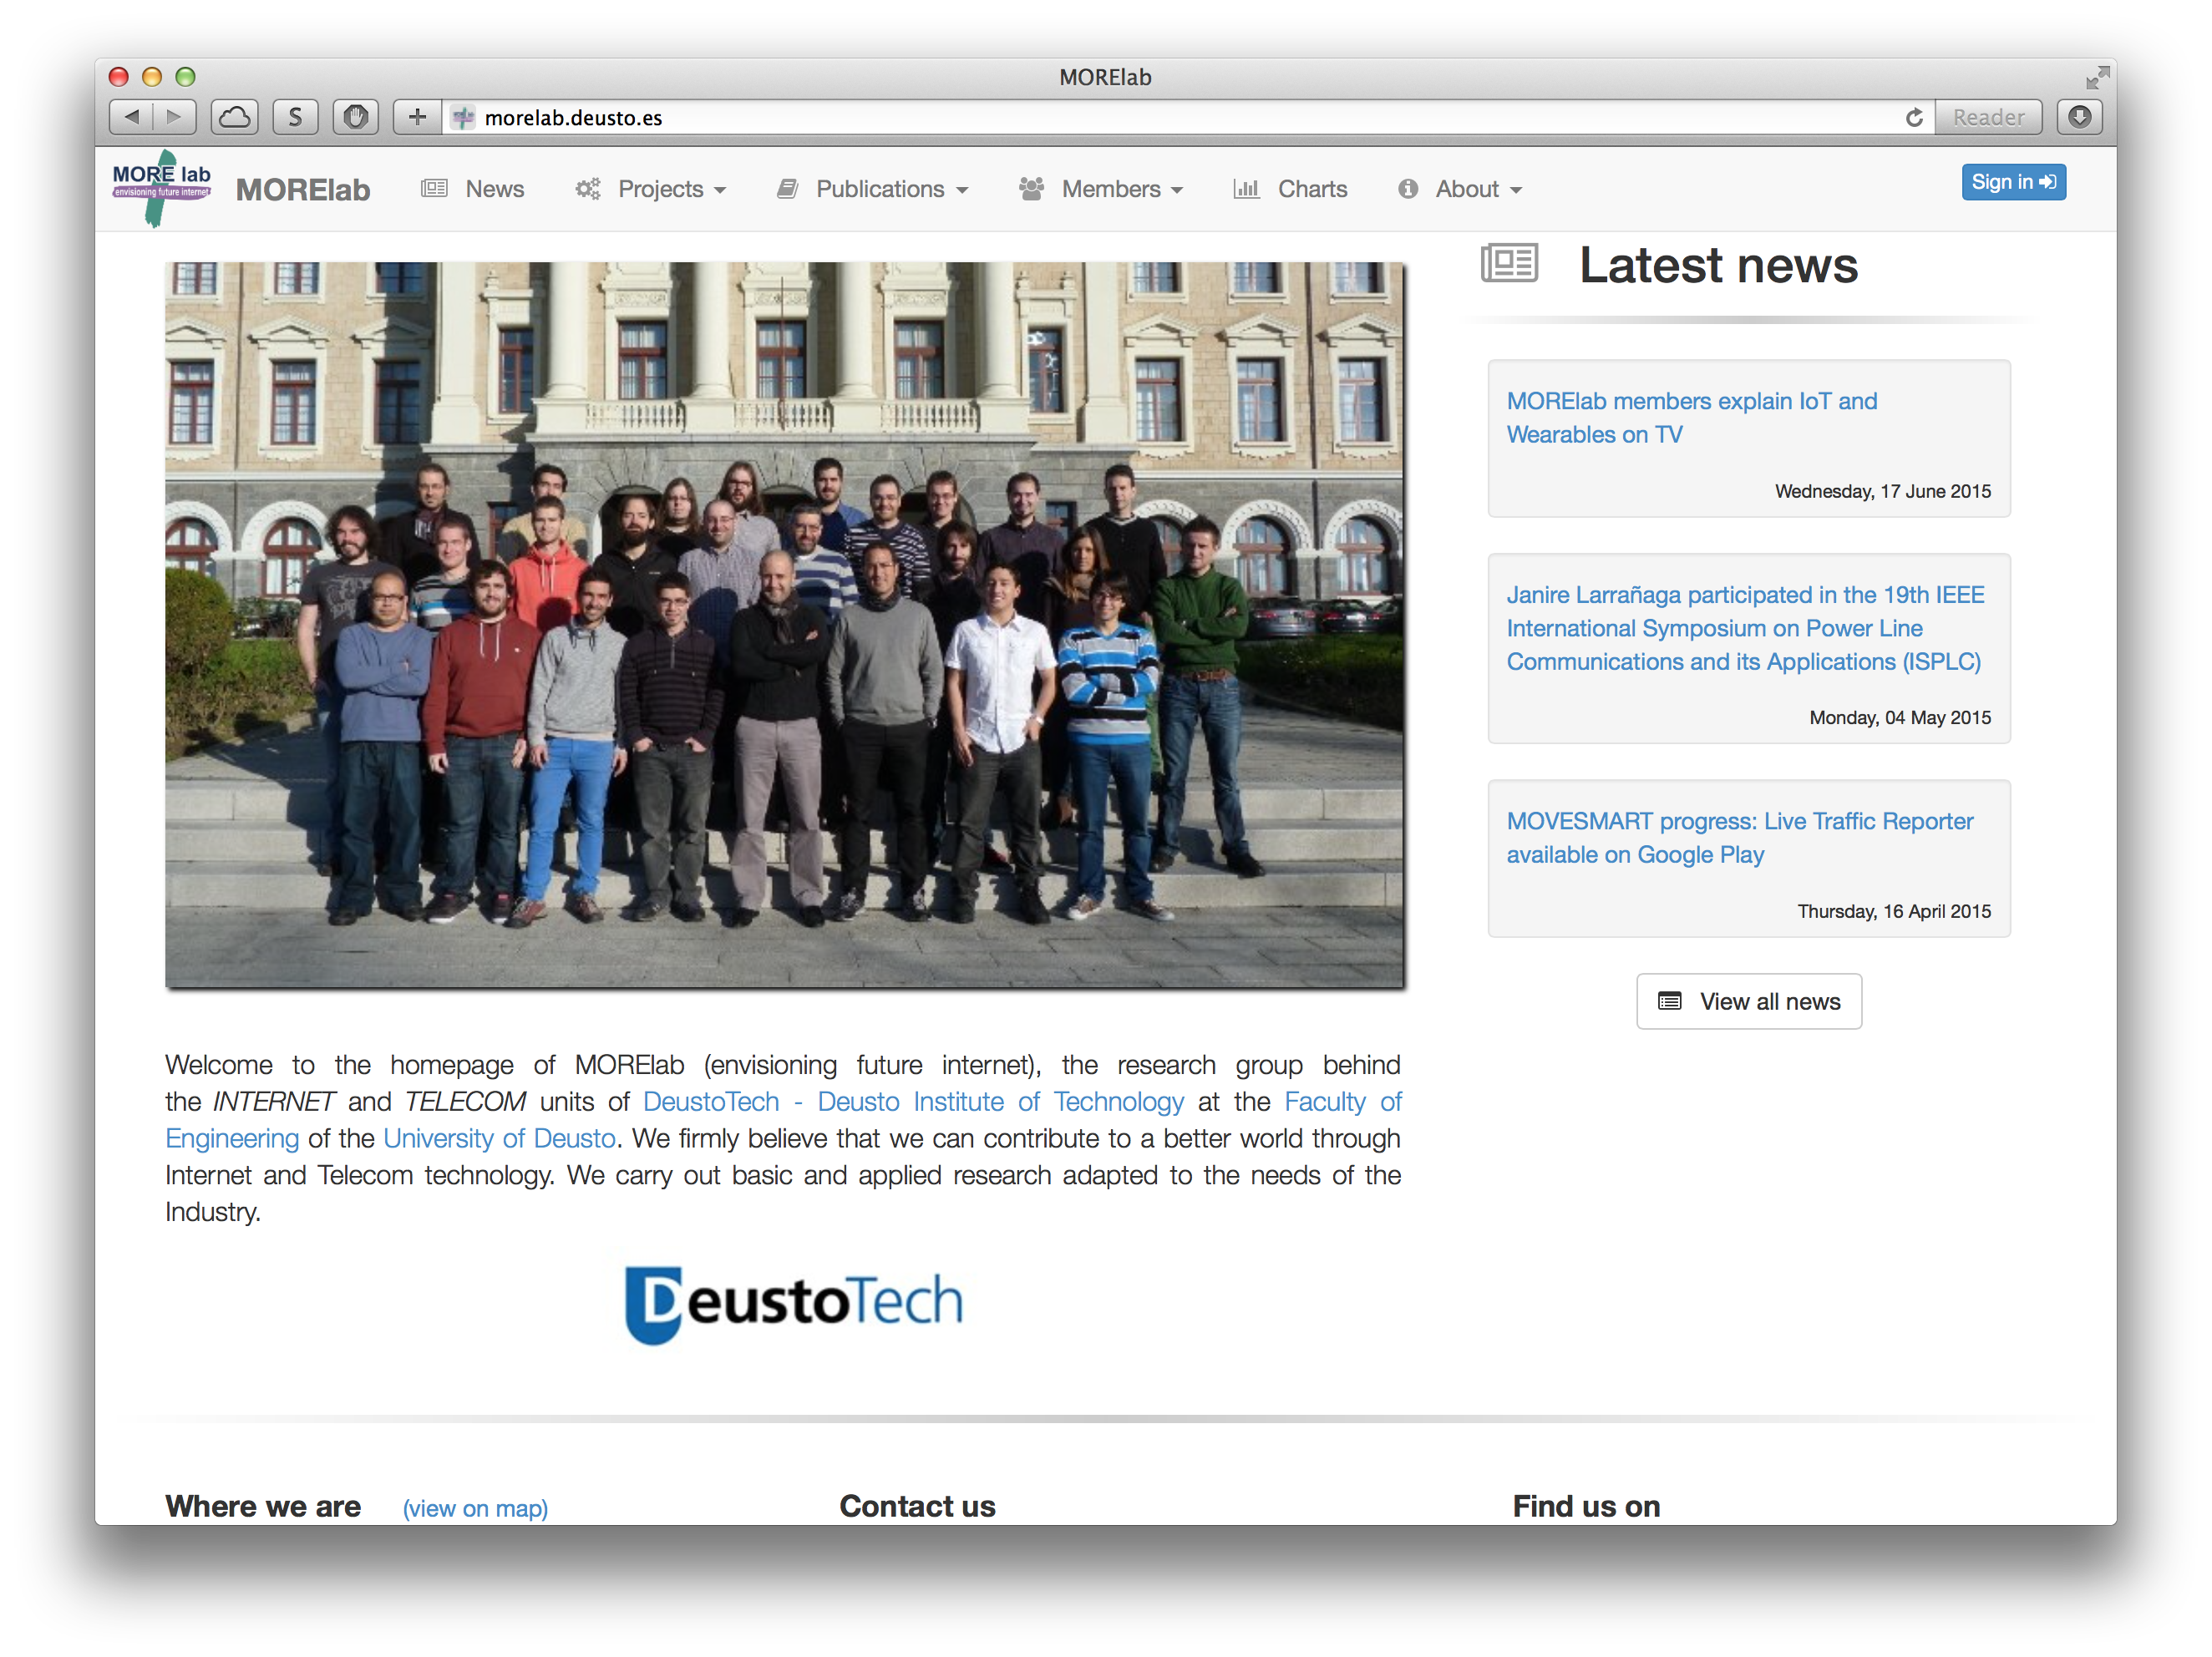
\includegraphics[scale=0.31]{fig/morelab_homepage}
	\caption{Página principal de \acrshort{labman} del equipo MoreLab}
	\label{fig:morelab_homepage}
\end{figure}

Este manual se centra en las opciones de \textit{Projects} y \textit{Publications}, dado que estas son las facetas en las que se ha trabajado a lo largo del proyecto y el resto están fuera del alcance.

\subsection{Projects: buscador de proyectos de LabMan}

Esta página muestra en principio la lista de todos los proyectos que involucran a los miembros del equipo de investigación sin filtrar. Mediante la barra de búsqueda para consultas sencillas (véase la figura \ref{fig:project_search_bar}), permite filtrar los proyectos por título o por el nombre del investigador que participe en los mismos.

\begin{figure}[!htbp]
	\centering
	
\includegraphics[scale=0.35]{fig/project_search_bar}
	\caption{Barra de búsqueda de consultas simples}
	\label{fig:project_search_bar}
\end{figure}

Sin embargo, al pulsar el botón con el símbolo \textbf{+} de la barra de búsquedas, se muestra un panel para realizar búsquedas avanzadas tal y como se muestra en la figura \ref{fig:projects_advanced_search}.

\begin{figure}[!htbp]
	\centering
	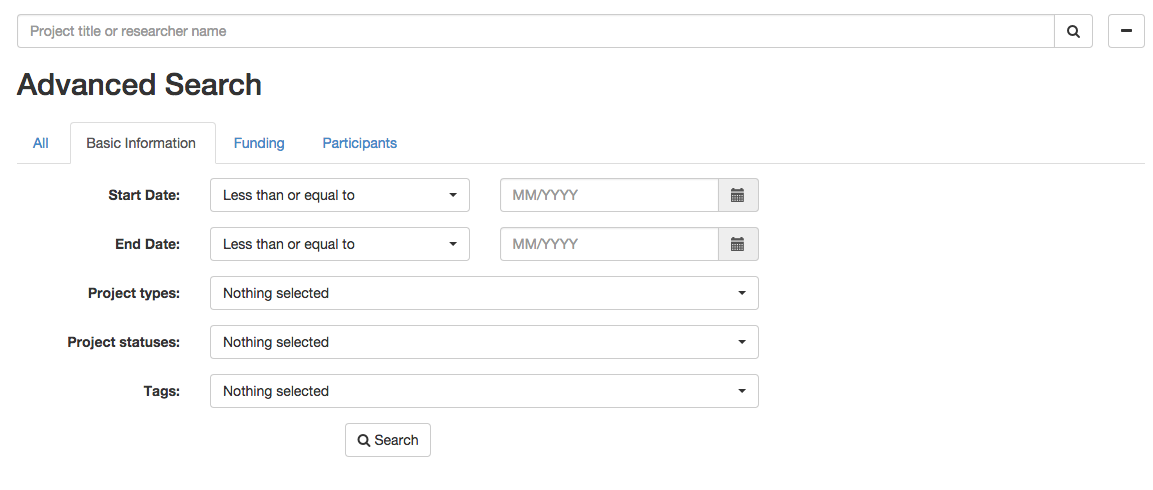
\includegraphics[scale=0.31]{fig/projects_advanced_search}
	\caption{Búsqueda avanzada de proyectos}
	\label{fig:projects_advanced_search}
\end{figure}

Mediante este buscador avanzado, se pueden filtrar los proyectos a partir de los siguientes características:

\begin{itemize}
	\item Basic information
	\begin{itemize}
		\item \textbf{Project title:} Busca todos los proyectos que contengan alguna de las palabras introducidas en este campo.
		\item \textbf{Start date:} Busca todos los proyectos que tengan una fecha de inicio menor, menor o igual, mayor, mayor o igual o igual a la introducida en este campo (formato MM/YYYY).
		\item \textbf{End date:} Busca todos los proyectos que tengan una fecha de fin menor, menor o igual, mayor, mayor o igual o igual a la introducida en este campo (formato MM/YYYY).
		\item \textbf{Project types:} Busca todos los proyectos que coincidan con alguno de los tipos de proyectos seleccionados en este campo.
		\item \textbf{Project statues:} Busca todos los proyectos que coincidan con alguno de los estados de proyectos seleccionados en este campo.
		\item \textbf{Tags:} Busca todos los proyectos que estén relacionados con alguno de las etiquetas seleccionadas en este campo.
	\end{itemize}
	\item Funding
	\begin{itemize}
		\item \textbf{Total funds:} Busca todos los proyectos cuya financiación total sea la cantidad en Euros especificada en este campo.
	\end{itemize}
	\item Participants
	\begin{itemize}
		\item \textbf{Member:} Busca todos los proyectos en los que haya participado los investigadores del grupo de investigación ejecutando alguno de los posibles roles seleccionados en este campo.
	\end{itemize}
\end{itemize}

Una vez se hayan definidos los valores de las características por las que se desea filtrar los proyectos se deberá pulsar el botón \textbf{Search} para comenzar la búsqueda y visualizar el resultado como puede mostrarse en la figura \ref{fig:projects_search_result}.

\begin{figure}[!htbp]
	\centering
	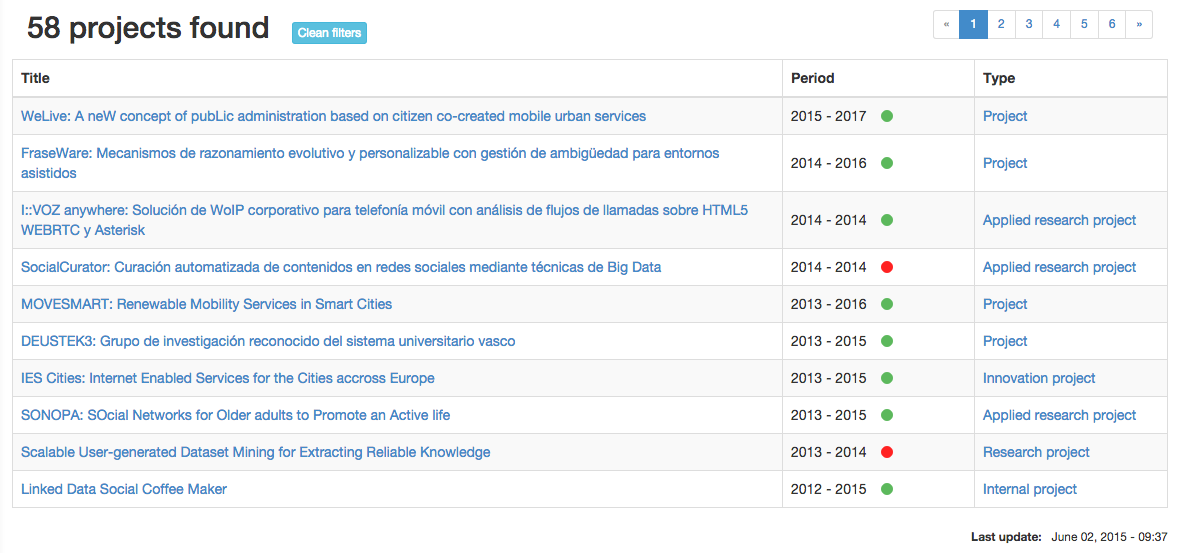
\includegraphics[scale=0.31]{fig/projects_search_result}
	\caption{Resultado de la búsqueda de proyectos}
	\label{fig:projects_search_result}
\end{figure}

\subsection{Publications: buscador de publicaciones de LabMan}

Esta página muestra en principio la lista de todos las publicaciones redactados por los miembros del equipo de investigación sin filtrar. Del mismo modo que con los proyectos, mediante la barra de búsqueda para consultas sencillas (véase la figura \ref{fig:publication_search_bar}), permite filtrar las publicaciones por título o por el nombre del investigador que ha contribuido a las mismas.

\begin{figure}[!htbp]
	\centering
	
\includegraphics[scale=0.35]{fig/publication_search_bar}
	\caption{Barra de búsqueda de consultas simples de publicaciones}
	\label{fig:publication_search_bar}
\end{figure}

Sin embargo, al pulsar el botón con el símbolo \textbf{+} de la barra de búsquedas, se muestra un panel para realizar búsquedas avanzadas tal y como se muestra en la figura \ref{fig:publications_advanced_search}.

\begin{figure}[!htbp]
	\centering
	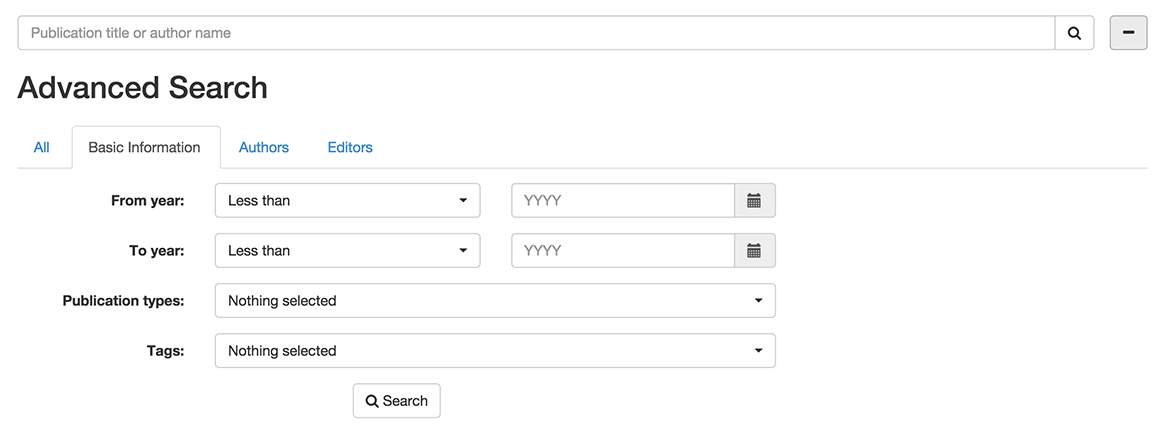
\includegraphics[scale=0.7]{fig/publications_advanced_search}
	\caption{Búsqueda avanzada de publicaciones}
	\label{fig:publications_advanced_search}
\end{figure}

Mediante este buscador avanzado, se pueden filtrar las publicaciones a partir de los siguientes características:

\begin{itemize}
	\item Basic information
	\begin{itemize}
		\item \textbf{Publication title:} Busca todos las publicaciones que contengan alguna de las palabras introducidas en este campo.
		\item \textbf{From year:} Busca todos los publicaciones que tengan un menor, menor o igual, mayor, mayor o igual o igual a la introducida en este campo (formato YYYY).
		\item \textbf{To year:} Busca todos los publicaciones que tengan un menor, menor o igual, mayor, mayor o igual o igual a la introducida en este campo (formato YYYY).
		\item \textbf{Publication types:} Busca todos las publicaciones que coincidan con alguno de los tipos de publicaciones seleccionados en este campo.
		\item \textbf{Tags:} Busca todos las publicaciones que estén relacionados con alguno de las etiquetas seleccionadas en este campo.
	\end{itemize}
	\item Authors
	\begin{itemize}
		\item \textbf{Author:} Busca todos las publicaciones que tenga a los investigadores del grupo de investigación seleccionados en este campo como autores.
	\end{itemize}
	\item Editors
	\begin{itemize}
		\item \textbf{Editor:} Busca todos las publicaciones que tenga a los investigadores del grupo de investigación seleccionados en este campo como editores.
	\end{itemize}
\end{itemize}

Una vez se hayan definidos los valores de las características por las que se desea filtrar los proyectos se deberá pulsar el botón \textbf{Search} para comenzar la búsqueda y visualizar el resultado como puede mostrarse en la figura \ref{fig:publications_search_result}.

\begin{figure}[!htbp]
	\centering
	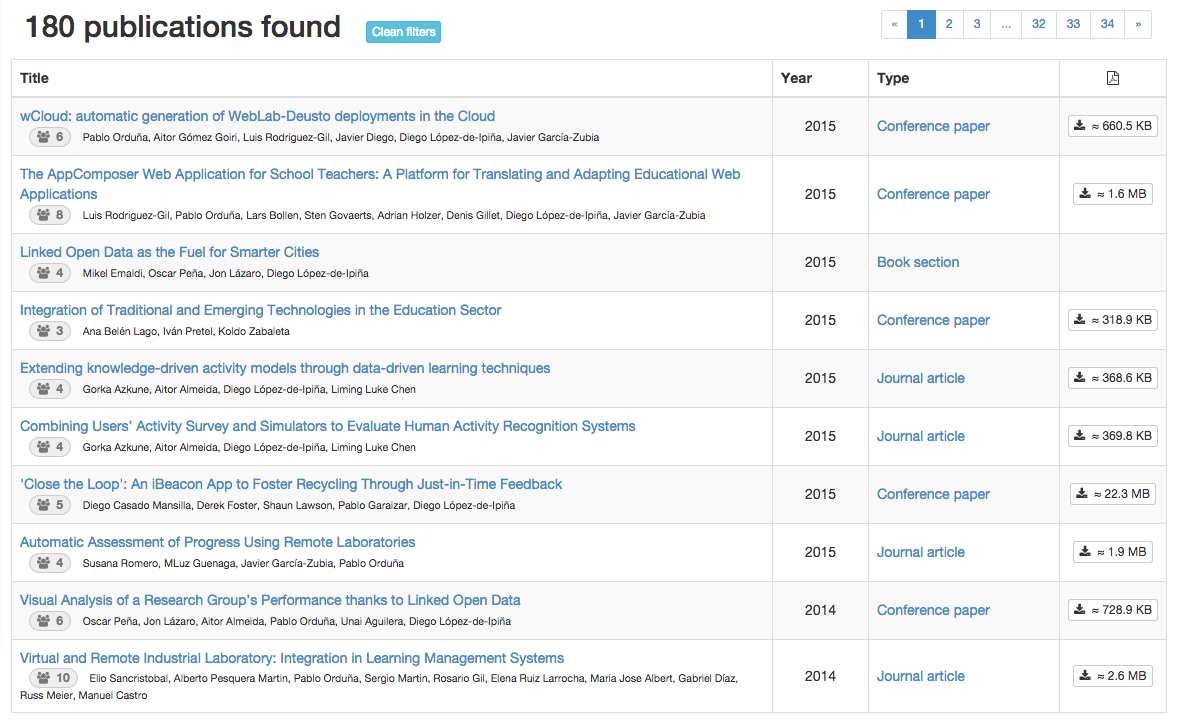
\includegraphics[scale=0.31]{fig/publications_search_result}
	\caption{Resultado de la búsqueda de publicaciones}
	\label{fig:publications_search_result}
\end{figure}

\chapter{Incidencias}

\section{Visión general}

Durante el desarrollo del proyecto han surgido diversas incidencias que han ralentizado el desarrollo de este. A continuación se van a explicar algunas de las más importantes, así como la decisión que se ha tomado en cada una de ellas.

\section{Instalación Graph models}

La instalación de la extensión de Django en OS X 10.9.8, Graph models ha sido larga y ardua. Para hacer uso de esta herramienta se ha tenido que instalar primeramente django-extensions, el cual no supuso ningún problema, dado que era una dependencia de \acrshort{labman} y se descargó e instaló durante el proceso de instalación de \acrshort{labman}. Creyendo que simplemente con instalar django-extensions era suficiente para la generación de los modelos se procedió a la ejecución de un comando de consola de ejemplo que venía con la instalación de \acrshort{labman}.

Al ejecutarlo se produjo un error informando que las herramientas pygraph o pydot no estaban instaladas, por lo que se procedió a instalar pygraph por medio gestor de paquetes de Python pip\cite{pip} a través del comando \textit{pip install pygraph} o bien \textit{easy\_install pygraph}, sin embargo o bien no lo encontraba o daba un error por faltar la dependencia graphviz.

Se intentó descargar la dependencia en primera instancia por medio de pip o easy\_install, aunque pudo no encontrar ningún paquete con dicho nombre. Como segundo intento se procedió buscar la dependencia por Homebrew\cite{Homebrew}, sin éxito alguno.

Se procedió como último intento a buscar en el repositorio web de MacPorts\cite{MacPorts} la existencia de graphviz y pygraph. Al verificar la existencia de estos paquetes en su repositorio, comenzó el proceso de descargar el paquete de instalación necesario para instalar MacPorts. Una vez instalado se introdujeron los comandos de instalación de ambos paquetes produciendose un error con el rsync. Al parecer, la Universidad de Deusto tiene algún puerto necesario para conectarse al repositorio cerrado por lo que se tuvo que crear un punto \acrshort{wifi} desde un dispositivo móvil conectado a una red privada \acrshort{3g} para descargar los paquete.

Al comenzar el proceso de instalación saltó una alerta sobre la ausencia de la herramienta de desarrollo Xcode\cite{Xcode} por lo que no se podrían compilar los paquetes. Se tuvieron que eliminar los archivos temporales que había generado MacPorts, descargar Xcode y aceptar la licencia de uso para finalmente poder instalar graphviz, lo que permitiría instalar por fin las dependencias pygraph y pydot para la ejecución del comando Graph models y generar los grafos adjuntados en esta memoria en el capítulo \ref{chap:design}.

\section{Despliegue del servidor OAI-PMH en Apache}

Antes del despliegue final en producción del servidor \acrshort{oaipmh} en el servidor \acrshort{http} Unicorn\cite{Unicorn}, se ha realizado un despliegue en un servidor Apache público para poder realizar pruebas con clientes \acrshort{oaipmh} web. No ocurrió ningún incidente durante el proceso de instalación de Apache en OS X, sin embargo la configuración fue tediosa.

En primer lugar se tuvo que localizar los ficheros de configuración y \textit{logs} del servidor Apache para OS X, estos se encontraban \textit{/etc/apache2} y \textit{/var/log/apache2} respectivamente.

Como el servidor de \acrshort{oaipmh} es una aplicación basada en \acrfull{wsgi} se tenía que modificar el fichero \textit{httpd.conf} para que el servidor Apache cargase el módulo necesario para la ejecución de este tipo de aplicaciones. Se siguió el tutorial de configuración rápida para mod\_wsgi (Módulo \acrshort{wsgi}) en la \textit{wiki} de la página del proyecto en Google Code\cite{GoogleCode} para hacer una aplicación de prueba y comprobar que el módulo se había cargado correctamente\cite{WSGI_tutorial}.

Se procedió a crear un \textit{VirtualHost} para hacer referencia al servidor \acrshort{oaipmh} por medio de una \acrshort{url}, sin embargo no se consiguió configurar adecuadamente, al hacer una petición por medio de un navegador web no se recibía respuesta alguna y el \textit{log} de Apache no registraba ningún error en las peticiones, por lo que se abandonó la idea de configurar el \textit{Virtual Host}.

Se optó por una solución menos elegante, pero así mismo funcional, se configuraría el \textit{WSGIScriptAlias} para poder hacer referencia a la aplicación \acrshort{wsgi} por medio de la dirección \acrshort{ip} de la máquina que ejecutaría el servidor desde un cliente externo al local.

Se intento realizar una nueva petición desde el navegador y esta vez si se obtuvo respuesta. Si bien no era la respuesta que se deseaba, al ser un error interno el servidor, la información de la petición quedó registrado en los \textit{logs}, por lo que fue más sencillo hacer un seguimiento hasta el origen del mismo. Se descubrió que Apache no ejecutaba el entorno virtual con el que se aislaba la instalación de Python y sus dependencias. 

A lo largo del desarrollo del servidor se habían utilizado varias versiones de Python como la 2.5, 2.6 y 2.7, trabajando la versión final en la 2.6. Sin embargo, Apache estaba ejecutando los fragmentos residuales del código desactualizado de la versión 2.7. Se estudiaron las posibles soluciones al problema y se decidió actualizar el código de la versión 2.7 con aquel desarrollado en la versión 2.6 tras descubrir que no había incompatibilidades en el código.

Tras realizar este cambio, el servidor fue desplegado correctamente. Se hicieron pruebas con clientes externos a la máquina local para comprobar que realmente se podía acceder al servidor y se procedió a realizar un redireccionamiento de puertos en el Router para hacer el servidor \acrshort{oaipmh} público y realizar las últimas pruebas con clientes web que requerían la \acrshort{url} del servidor para descargar los datos y realizar las validaciones.

\section{Escapar caracteres especiales de JSON}

Gracias a las pruebas unitarias realizadas en el método \textit{oai\_query} que se tuvo que implementar en la capa de \acrshort{bd} del servidor MOAI se descubrió que varios de los campos recolectados podían contener caracteres de control como los que se muestran en la figura \ref{fig:json_string}.

\begin{figure}[!htbp]
	\centering
	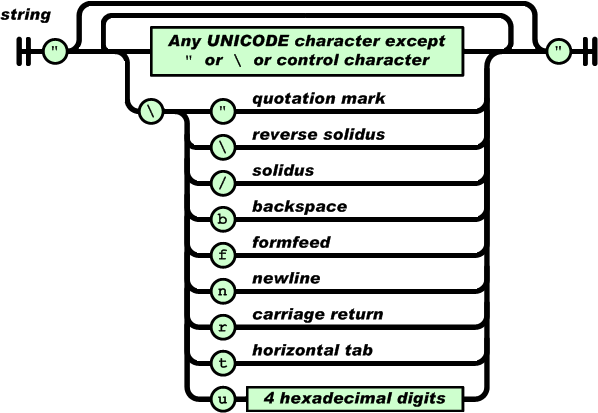
\includegraphics[scale=0.5]{fig/json_string}
	\caption{Definición de ``string'' de \acrshort{json}}
	\label{fig:json_string}
\end{figure}

Para evitar que surgieran errores se tuvo que implementar un método que eliminase estos caracteres te control o los escapase tal y como se muestra en el algoritmo \ref{lst:escaping_control_characters}

\lstinputlisting[language=Python, frame=single, label={lst:escaping_control_characters}, caption=Escapado o eliminación de caracteres de control de \acrshort{json}]{content/code/python/escaping_control_characters.py}

\chapter{Conclusiones y líneas futuras}

\section{Visión general}

Este capítulo contiene las conclusiones que se han obtenido después de haber desarrollado el proyecto y las posibles acciones que se podrían tomar de cara al futuro para mejorarlo.

\section{Objetivos cumplidos}

A pesar de no haber dispuesto de tanto tiempo como se hubiese deseado para la realización del proyecto, se podría considerar que los objetivos del proyecto han sido cumplidos, tal como se definen en el capítulo correspondiente.

\begin{itemize}
	\item Se ha añadido compatibilidad con \acrshort{oaipmh} al sistema de gestión de grupos de investigación \acrshort{labman}.
	\item Se ha expandido \acrshort{labman} con un buscador avanzado que permita buscar y filtrar entre los distintos proyectos y publicaciones.
\end{itemize}

Por otro parte, los requisitos definidos del software han sido cubiertos:

\begin{itemize}
	\item El servidor permite transformar datos almacenados en una base de datos relacional en \acrshort{xml} respetando la especificación del esquema bibliográfico \acrshort{dc}.
	\item El servidor permite visualizar la información como \acrshort{xml} en texto plano en navegadores web convencionales.
	\item El servidor genera los \textit{sets} sobre cada uno de los tipos de publicaciones para facilitar la recuperación de metadatos selectiva.
	\item En la aplicación web, el formulario extendido de búsquedas avanzadas debe estar oculto inicialmente para permitir realizar consultas sencillas rápidamente.
	\item El buscador permite realizar búsquedas por rango entre dos fechas o establecer una fecha específica.
	\item La aplicación mantiene el \textit{Look and Feel} originario de \acrshort{labman}, su diseño y elementos básicos hacen uso o se basan en los componentes facilitados por Bootstrap 3.
	\item Los elementos del buscador avanzado han de ser responsivos para ser adaptable en diferentes dispositivos, como ordenadores de sobremesa, tabletas y móviles.
	\item Las distintas secciones en la que se dispone el buscador de publicaciones y proyectos tienen un diseño intuitivo para facilitar su uso. 
\end{itemize}

\section{Conclusiones}

Lo que al principio parecía un proyecto difícil, dado que en un comienzo no se conocía en que consistía el protocolo \acrshort{oaipmh} y se tuvo que adentrar en el gran mundo de los estándares para las publicaciones bibliográficas digitales. Se tuvo que realizar un estudio exhaustivo entre las tecnologías que facilitaba la comunidad de \acrshort{oai} y encontrar alguna que permitiera modificar la base de datos por defecto del proveedor de datos. Muchos de estos servidores no permitían dicha modificación lo que suponía tener que duplicar todos los datos del repositorio actual de \acrshort{labman}, siendo esta solución inviable. Había que buscar un servidor que facilitara una \acrshort{api} para extender o añadir la \acrshort{bd} por defecto de la herramienta, en caso contrario habría que plantearse en desarrollar un servidor \acrshort{oaipmh} por completo.

Por suerte se descubrió MOAI, una aplicación basada en \acrshort{wsgi} compatible con el protocolo \acrshort{oaipmh} que permitía añadir una \acrshort{bd} personalizada y ahorrar todo el tiempo de desarrollo que hubiera supuesto tener que desarrollar un servidor \acrshort{http} que cumpliera con todos los requisitos por completo.

De esta forma se pudo adaptar MOAI para reutilizar el modelo de datos relacional que usaba \acrshort{labman} y dedicar el tiempo a diseñar cuales de estos campos del modelo podían ser usados cumpliendo la especificación del estándar bibliográfico \acrshort{dc}.

Por otra parte, al decidir utilizar MOAI se ha tenido que dedicar un tiempo extra a aprender en profundidad el lenguaje de programación Python, dado que hasta la fecha solo se sabía, como mucho, interpretar el código. De todas formas el tiempo dedicado a la asimilación de Python no ha sido en vano, dado ha posibilitado el descubrir un lenguaje con un gran potencial.

Es necesario destacar lo mucho que se ha aprendido del desarrollo de aplicaciones web en Python con la puesta en producción del servidor \acrshort{oaipmh}, así como las pruebas previas realizadas para hacer el servidor público mediante Apache, así como con el desarrollo del \textit{back-end} de la extensión de \acrshort{labman} en Django. Estas tecnologías, si bien no son las más novedosas como NodeJS\cite{NodeJS} o AngularJS\cite{AngularJS}, si son algunas de las más usadas y asentadas, permitiendo contribuir con grandes proyectos implantados con esta tecnología.

En conclusión, el desarrollo y estudio de este proyecto no ha resultado fácil, aunque se han aprendido mucho con el uso de estas tecnologías, además del contexto relacionado al campo de la investigación académica que seguro que resultarán de utilidad en futuros proyectos.

\section{Líneas Futuras}

Existen diversas funcionalidades que se podrían añadir al proyecto en un futuro y que aumentarían la calidad de este de una forma considerable:

\begin{itemize}
	\item Se debería modificar el modelo de datos relacional del repositorio de \acrshort{labman}, que permita almacenar la fecha de creación o modificación de los recursos. El protocolo de \acrshort{oaipmh} requiere conocer dicha fecha para mostrar los recursos delimitados por los parámetros \textit{from} y \textit{to} en las consultas \textit{ListIdefitiers} y \textit{ListRecords}. Esto aumentaría la eficiencia y el tiempo de respuesta del servidor evitando la ardua tarea que consultar los \textit{logs} de administración de Django en busca de cambios para actualizar la última fecha de modificación por cada uno de los recursos del dispuestos por el servidor \acrshort{oaipmh}.
	\item En el cliente web, se podría añadir la funcionalidad para que la tabla que contiene el resultado de las consultas pudiera reorganizar las columnas, posibilitar el cambio del orden ascendente o descendente en las mismas, etc. Todo esto de la forma más eficiente posible mediante la definición de un sistema de cacheo de los recursos, reduciendo tiempo de generación de la respuesta y la cantidad de datos web consumidos.
\end{itemize}


\printbibliography[heading=bibintoc]
\printglossary[type=\acronymtype, title=Acrónimos, toctitle= Acrónimos]

\appendix

\chapter*{Agradecimientos}
\addcontentsline{toc}{chapter}{Agradecimientos}

No podríamos dar finalizada la memoria del presente proyecto, sin agradecer a todos aquellos que me han apoyado u ofrecido su ayuda durante estos meses de arduo trabajo.
En especial quisiera dar las gracias a: 

\begin{itemize}
	\item \textbf{Mi padre, Abilio}, que ha sacrificado 46 años de su juventud trabajando para poder ofrecerme la posibilidad realizar estos estudios académicos. Pero además me ha apoyado y dado ánimos en los momentos más duros, en los que de no ver sino por él hubiera tirado la toalla.

	\item \textbf{Mi madre, Begoña}, que aunque muchas veces no la haya valorado siempre ha estado ahí preocupandose por mí, haciendome la vida más cómoda de un modo u otro. De no haber sido por su insistencia, y de todas esas horas que ha pasado cerca de mi apoyandome en lo que ha podido, dejando sus tareas de lado, no hubiera podido llegar a donde estoy.

	\item \textbf{Aritz Bilbao Jayo}, compañero y amigo de gran corazón, que desde que lo conocí en primero de carrera no ha dejado de sorprenderme de sus capacidades y de lo tremendamente humano que es. Se ha preocupado por mí y me ha ayudado durante toda la carrera resolviendome las dudas que me hayan podido surgir, que cada vez van en aumento lamentablemente. 
	Además fue él quien me recomendó para trabajar en MORElab y quien que me introdujo en el desarrollo web, sin él no hubiera podido avanzar tan deprisa.
	
	Espero seguir pasando buenos momentos junto a él durante venideras ediciones de la Euskal encounter. Sin duda se merece una TARDIS.

	\item \textbf{Iban Eguia Moraza}, preciado amigo que me a apoyado en tiempos difíciles de la carrera. Es además un sorprendente hombre con una capacidad por encima de la media que me ha enseñado las virtudes del \textit{Open-source}. Su último gran consejo, a la hora de redactar estas lineas, fue el convencerme de utilizar \hologo{LaTeX}, que de muchas horas de quebraderos de cabeza me ha librado.
	
	Más importante aún, me ha enseñado a valorar a los que me rodean y a ser más humano y sociable, cualidades que aún tengo que esforzarme en potenciar.

	\item \textbf{Diego López-de-Ipiña González-de-Artaza}, No solo ha sido el director de este proyecto, sino que ha demás ha sido mi mentor en asignaturas como \textit{Software Process and Quality} y \textit{Desarrollo Avanzado de Software} que me ha enseñado las tecnologías que están en auge en el ámbito del desarrollo web además de ofrecerme los conocimientos básicos y fundamentales de las mismas. Si no huera creído en mí, todos proyectos en los que he participado y de los que tanto he aprendido no hubieran sido posibles.

	\item \textbf{Oscar Peña}, desarrollador del \acrshort{dms} del equipo de MORElab de Deustotech del cual se basa mi proyecto. Gracias a él pude enterarme de las tecnologías que tenía que utilizar para realizar el proyecto y me ayudó a asimilar y comprender el diseño de la base de datos de LabMan para el desarrollo del servidor de \acrshort{oaipmh} así como en el proceso de instalación del servidor de LabMan y a trabajar con Django en general.

\end{itemize}

\backmatter

\end{document}
